% REMEMBER: You must not plagiarise anything in your report. Be extremely careful.

\documentclass{l4proj}
\graphicspath{ {./images/} }
    
%
% put any additional packages here
%
\usepackage{siunitx}
\usepackage[table,xcdraw]{xcolor}
\usepackage{tablefootnote}
\begin{document}

%==============================================================================
%% METADATA
\title{Digital Multilingual News Surveillance and Classification System}
\author{Adam Fairlie}
\date{March 24, 2023}

\maketitle

%==============================================================================
%% ABSTRACT
\begin{abstract}
    Current digital news surveillance systems for disease monitoring lack diversity in their data collection systems, and require results to be translated into English before processing. We developed a more robust data collection system which integrates various types of online data into one system, as well as a web interface to manage the system and view result visualisations. Various multilingual machine learning techniques were explored in an experiment on multilingual news category classification, and a classifier to assign categories to incoming multilingual articles was trained and integrated into the collection system. The classifier achieves 89.4\% accuracy on real-world collected data
\end{abstract}

%==============================================================================

% EDUCATION REUSE CONSENT FORM
% If you consent to your project being shown to future students for educational purposes
% then insert your name and the date below to  sign the education use form that appears in the front of the document. 
% You must explicitly give consent if you wish to do so.
% If you sign, your project may be included in the Hall of Fame if it scores particularly highly.
%
% Please note that you are under no obligation to sign 
% this declaration, but doing so would help future students.
%
\def\consentname {Adam Fairlie} % your full name
\def\consentdate {24 March 2023} % the date you agree
%
\educationalconsent


%==============================================================================
\tableofcontents

%==============================================================================
%% Notes on formatting
%==============================================================================
% The first page, abstract and table of contents are numbered using Roman numerals and are not
% included in the page count. 
%
% From now on pages are numbered
% using Arabic numerals. Therefore, immediately after the first call to \chapter we need the call
% \pagenumbering{arabic} and this should be called once only in the document. 
%
% Do not alter the bibliography style.
%
% The first Chapter should then be on page 1. You are allowed 40 pages for a 40 credit project and 30 pages for a 
% 20 credit report. This includes everything numbered in Arabic numerals (excluding front matter) up
% to but excluding the appendices and bibliography.
%
% You must not alter text size (it is currently 10pt) or alter margins or spacing.
%
%
%==================================================================================================================================
%
% IMPORTANT
% The chapter headings here are **suggestions**. You don't have to follow this model if
% it doesn't fit your project. Every project should have an introduction and conclusion,
% however. 
%
%==================================================================================================================================
\chapter{Introduction}

% reset page numbering. Don't remove this!
\pagenumbering{arabic} 

\section{Motivation}

The rate of transmission in diseases is often high, travelling rapidly between areas before it can be initially detected and contained. It is important to avoid as much harm as possible by having up-to-date information on local disease outbreak risks freely available to members of the public. Traditional methods of disease surveillance include laboratory networks such as PulseNet from the Center for Disease Control (CDC) which look for patterns in bacteria across infected patients which may indicate an outbreak. These methods can be slow, relying on human experts and conducting experiments which can take several days until results are achieved \citep{swaminathan2001pulsenet}. These methods are often also lacking in coverage of certain diseases or geographic regions due to factors such as a lack of specialist knowledge \citep{abdulraheem2004disease}. Digital forms of surveillance such as online media monitoring have been effective at discovering disease outbreaks at the early stages and mitigating spread, including during the recent COVID-19 pandemic \citep{kostkova2021data}. Several digital surveillance systems have been developed to collect real-time information from online sources, such as news articles, which can be used to quickly find and assess the risk of disease outbreaks across the world. This information can allow governments to respond rapidly to any new outbreaks by providing quick risk information to the public and planning for diagnosis, testing and prevention. It is for this reason that many governments are creating systems which incorporate online sources to monitor disease outbreaks, such as the Global Public Health Intelligence Network (GPHIN)\footnote{https://gphin.canada.ca/cepr/aboutgphin-rmispenbref.jsp?language=en\_CA} from the Canadian government. \par

One such digital surveillance system is BioCaster\footnote{http://biocaster.org/}, developed by a research team from the University of Cambridge and McGill University, which collects news data and provides an online visualisation of disease alerts on their website. There are flaws with the current BioCaster system, particularly in the news collection system. The current system relies on published news feeds, typically provided by large established sources in high-resource countries, creating a coverage gap in low-resource areas and minority languages. The lack of diversity in the types of sources collected may also impact countries which publish less traditional news, and restricts types of online data such as search trends and social media posts which research has shown to be effective in detecting disease outbreaks early \citep{seo2017methods}. \par
Another weakness in the current BioCaster system is the reliance on the accuracy of external machine translation systems to translate all documents to English before disease risk can be calculated. These systems can struggle with issues such as domain mismatch (words having different translations depending on the domain) \citep{koehn2017six} and can encode forms of bias such as gender bias \citep{stanovsky2019evaluating}. Multilingual models which eliminate the need for machine translation exist for tasks such as multiclass classification, and have not been tested within the BioCaster system.

\section{Project Aims}
This project develops a new digital surveillance system for multilingual news data, which aims to improve aspects of the existing BioCaster system. The new system developed should have the following aspects: 
\subsection{Digital News Surveillance System} \hfill \par
\subsubsection{News collection system}
This project will develop a robust and extensible data collection system which can synthesise data from multiple different sources and source types, allowing for a more extensive selection of online news data to be collected including lower-resource countries and minority languages. The project will implement two distinct methods of data collection: RSS\footnote{Really Simple Syndication} feeds and web scraping. It will redevelop an improved version of the current BioCaster data collection system based on RSS feeds so that the current system can integrate into the new system without loss of data sources. A web scraping system will also be developed to extract important information such as article headlines, main bodies and publish dates from a given webpage.
\subsubsection{Data storage and visualisation} The collected news data will be stored in structured form in a database. The information will then be used to produce real-time visualisations of collected data, aggregated into useful statistics, graphs and charts, so that data collected can be observed and analysed. These visualisations should include information on the source countries and languages of collected data, the methods of collection used to retrieve the data and the category distributions of news articles. The system should frequently update and be easy to understand.
\subsubsection{Web interface} A web interface will be developed so that the data collection system can be easily managed, including enabling/disabling data sources, and adding and removing sources. The system should display the last time sources have collected new data, allowing for the highlighting of stale sources which can be removed to save resources. The interface should be responsive and easy to use and understand.
\subsection{Multilingual News Article Classification} \hfill \par
We will also conduct research on multilingual machine learning models through the task of multilingual news article category classification, training on public news article datasets and collected real-world news data, and evaluating the accuracy of multilingual models and the effectiveness of machine translation techniques on upsampling datasets. In particular, I will research the effectiveness of machine translation as an upsampling technique, the effectiveness of models trained on public data when translated to real-world data and the current effectiveness of multilingual models on real-world news data. The final multilingual classifier will be integrated into the scraping system, assigning each incoming article a category.

%\section{Chapter outline}
%This chapter outlines the motivation behind the project and some of the key goals. Future chapters will provide more detail on the exact system design and implementation, and evaluate how effectively the system meets these proposed goals. The paper structure is as follows:
%\begin{itemize}
%\item \textbf{Chapter 2} covers research into existing digital surveillance systems, real-time data visualisation systems and the currently available news datasets and approaches to news article classification. 
%\item \textbf{Chapter 3} covers the high-level system design of the overall system and its components, and describe the plan for experiments related to multilingual multiclass news article classification.
%\item \textbf{Chapter 4} covers the experiments performed in order to evaluate multilingual models through the classification task.
%\item \textbf{Chapter 5} covers the exact implementation details of the system, and the exact process for data collection and training of multilingual classifier models.
%\item \textbf{Chapter 6} presents the results of the evaluations to consider whether the system achieves its goals. These evaluations are the usability tests for the visualisation and web interface, and the results of training the multilingual classifiers.
%\item \textbf{Chapter 7} summarises and reflects on the project and considers future work which could be carried out to extend or improve certain aspects.
%\end{itemize}

%==================================================================================================================================
\chapter{Background}
\section{Digital News Surveillance Systems}

Several digital news surveillance systems exist for different purposes, including research systems for public health monitoring and commercial systems designed for businesses to track information related to their brand. HealthMap\footnote{https://www.healthmap.org/en/} is a public health monitoring system which provides a world map with location-based disease markers for each country, using RSS data and sources gathered by health experts. EpiCore \citep{haddad2016epicore} is a similar system but instead uses an online network of trained experts to share information digitally. MediSys \citep{steinberger2008medisys} is a public health monitoring system which takes information from many web portals and commercial news sites to sort incoming news into topics which can be viewed on the website. \par

\subsection{BioCaster}
This project reworks and extends some of the functionality currently used in BioCaster. The BioCaster system collects news articles through a variety of RSS (Really Simple Syndication) feeds across different languages including English, French and Mandarin \citep{collier2008biocaster}. It uses a machine translation server to translate the headlines and article descriptions into English, and various machine learning and rule-based models to filter the English-language data to remove all irrelevant (not disease-related) articles and collect specific details which are used to create a risk alert. These alerts are displayed in a visualisation on the website. A full diagram of the BioCaster system architecture is shown in Figure \ref{fig:biocaster_architecture}. 
 \begin{figure}[h]
 \centering
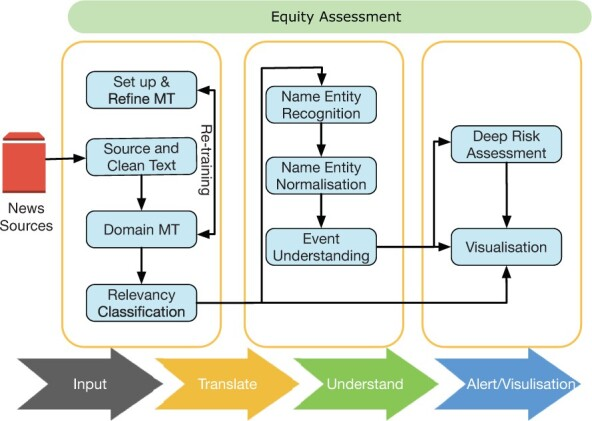
\includegraphics[width=0.75\textwidth]{/biocaster_diagram.jpg}
\caption{The full architecture of the current BioCaster app. Image obtained from \cite{meng2022biocaster}}
\label{fig:biocaster_architecture}
\end{figure}
\par

This project aims to rework the first part of this architecture, improving the quality of news sources and removing the machine translation steps. The current BioCaster data collection method is dated: it has not been updated in many years and only collects data through RSS feeds, by running a Perl script once per hour to receive updates \citep{collier2008biocaster}. This requires a news source to publish and maintain a feed for its data to be used in the system. These feeds are provided by a limited number of news sources, which are typically larger and written in high-resource languages and countries, where data is not as underrepresented. This greatly limits the amount of data which can be extracted, particularly from smaller sources in underrepresented countries and minority languages, and as RSS technology is becoming more outdated and falling out of use, the data available for use in surveillance is continuing to diminish in the current system. The data collected from RSS feeds is also limited to a headline and in some cases a short or medium-length description of article content. This provides limited information to models in later stages of the process for performing relevance classification and risk alert creation tasks. \par
The current BioCaster system also heavily relies on external domain machine translation. These models can suffer when trained on data outside of their domain \citep{koehn2017six}, possibly resulting in inaccurate translations as we cannot expect all news collected to be strictly biomedical. The reliance on external resources can also impact the availability of the service, removing some of the control from the BioCaster team. \par
This project will update the BioCaster RSS collection system, as well as add a module for using web scraping to collect news articles from webpage HTML. The system will be designed so that it is easily extensible to other sources of data which may be more prominent in different countries than traditional news, such as social media posts. This also allows for entire article text to be collected instead of just the headline and a short description, which may allow for a richer understanding of the news content and more effective performance in ML tasks. It will also experiment with multilingual news article classification techniques to remove the problems associated with relying on machine translation servers.

\section{Multilingual News Article Classification}
\subsection{Traditional Models}
Historically, many different approaches and models have been used for the task of news article category classification. The most popular model types before the last 5 years are Support Vector Machines (SVM's) and Naive Bayes classifiers. SVM's are models which aim to split the input space into different categories with as large a margin as possible, by finding the best possible hyperplanes in high-dimensional space which split the data into their correct classes. SVM models can achieve non-linearity by transforming inputs through a kernel,n a function which transforms inputs into a space which can be linearly separated by the hyperplanes. SVM Models have been repeatedly demonstrated to perform with high accuracy in the news classification literature across different languages, achieving 90+\% accuracy on categorisation of news headlines from Sri Lanka \citep{dilrukshi2013twitter} and 85\% accuracy on news documents from Indonesian news source Kompas \citep{liliana2011indonesian}. \par
Naive Bayes classifiers take in input features, which are (usually incorrectly) assumed to be independent for simplicity, and uses them to update a prior belief about how class data is distributed until the distribution reflects the distribution of real data as accurately as possible. Naive Bayes models are probabilistic models, meaning instead of assigning a single class to an output, it creates a probability distribution over all possible classes which can be sampled from for a particular input. A common strategy for Naive Bayes classifiers is to simply take the class with the highest probability for a given input (maximum a posteriori decision rule). The assumption of independence in features can be problematic for classifying news documents, which have heavily codependent features, but methods have been developed to mitigate this issue \citep{qiang2010effective}.Naive Bayes models have produced impressive results on an Indonesian news dataset, achieving 94\% accuracy \citep{septian2017indonesian} and 87\% accuracy on English-language Indian news \citep{kumar2022intelligent}.
SVM models typically achieve higher accuracy than Naive Bayes models because of the weakness of Naive Bayes inappropriate assumption of independence \citep{dilrukshi2013twitter2, shahi2018nepali, fanny2018comparison}, but Naive Bayes models have the advantage of initialising and classifying data faster than SVM models due to their simplicity, and can sometimes provide comparable or better results.\citep{ting2011naive}. Other traditional models used in news classification include random forests, which create decision trees in order to discriminate between categories \citep{liparas2014news} and K-NN classifiers, which takes the K most similar documents and assigns the article the most common class of these documents \citep{chen2020lao}.

\subsection{Transformer Models}
While these traditional models achieved very high performance on many monolingual datasets, there was often a significant decrease in more complex tasks such as classifying multilingual data \citep{vogel2020detecting}. In 2017, the Google research team released the transformer model architecture, which revolutionised text classification for allowing the context of words within a sentence to be leveraged in the model calculations \citep{vaswani2017attention}. A further development BERT, a bi-direction sequence-to-sequence model which removed the decoder section in order to learn word embeddings \citep{devlin2018bert}. BERT very quickly outperformed many established baselines and became the state-of-the-art, and is very widely used in news classification in the last 5 years \citep{chen2022long, mujahid2021classification, deping2021news}, . A detailed explanation of the transformer and BERT architectures can be found in section \ref{section:preliminaries}. These models are widely used because they are pre-trained, and only require fine tuning to a specific task, massively saving computation time and allowing for public access to very complex models, allowing the task of multilingual news classification to be attempted more effectively.

BERT-based models exist which are trained on a corpus of multilingual data, and can embed and represent multilingual input data for classification tasks. One of the most popular multilingual models is mBERT, or multilingual BERT, a variant of BERT trained on over 100 languages. Research by \cite{pires2019multilingual} suggests mBERT may learn an effective language-agnostic latent space which yields impressive results when the model is evaluated on different languages than it is trained on, but this effect decreases as the languages become less structurally similar. mBERT has been used to high success in multilingual news classification tasks \citep{kakwani2020indicnlpsuite, hutama2022indonesian} \par
Another model is XLM-RoBERTa, developed by the Facebook AI team \citep{conneau2019unsupervised}. It has been shown to outperform mBERT in many multilingual tasks such as named entity recognition (NER) and relation extraction \citep{li2021cross, lan2020empirical}, as well as in news classification \citep{alam2020bangla}. These two models will be considered in our evaluation, as they represent the current state-of-the-art in multilingual news classification.

%==================================================================================================================================


\chapter{System Design}
\section{Design Principles}
The system architecture was designed with consideration towards a few key software design principles and concepts. The main influences and aims of the overall system design are:
\begin{itemize}
    \item \textbf{Separation of concerns: } Each individual component of the system is given its own module which encapsulates its main functionality and interaction with other modules. This also means that components could possibly be re-used in future projects.
    \item \textbf{Configurability: } The system is designed to give the user as much choice as possible. The system can read a config file which allows the user to control many aspects of the system, such as whether a local or cloud database is used and the maximum number of active sources which are loaded. In addition, individual components are designed so that they can easily be switched out if new components are developed.
    \item \textbf{Extensibility: } Modules of the system which can have implementations changed or new versions created are designed so that this process is as easy as possible, abstracting the consistent functionality of the module into a superclass that new components will inherit from. As previously discussed, social media data has been shown to be a powerful indicator of disease outbreaks, so this system could be extended by adding a social media crawler, for example.
\end{itemize}

\section{System Overview}
Figure \ref{fig:system_overview_diagram} shows a diagram of the overall system architecture.
 \begin{figure}[h]
\centering
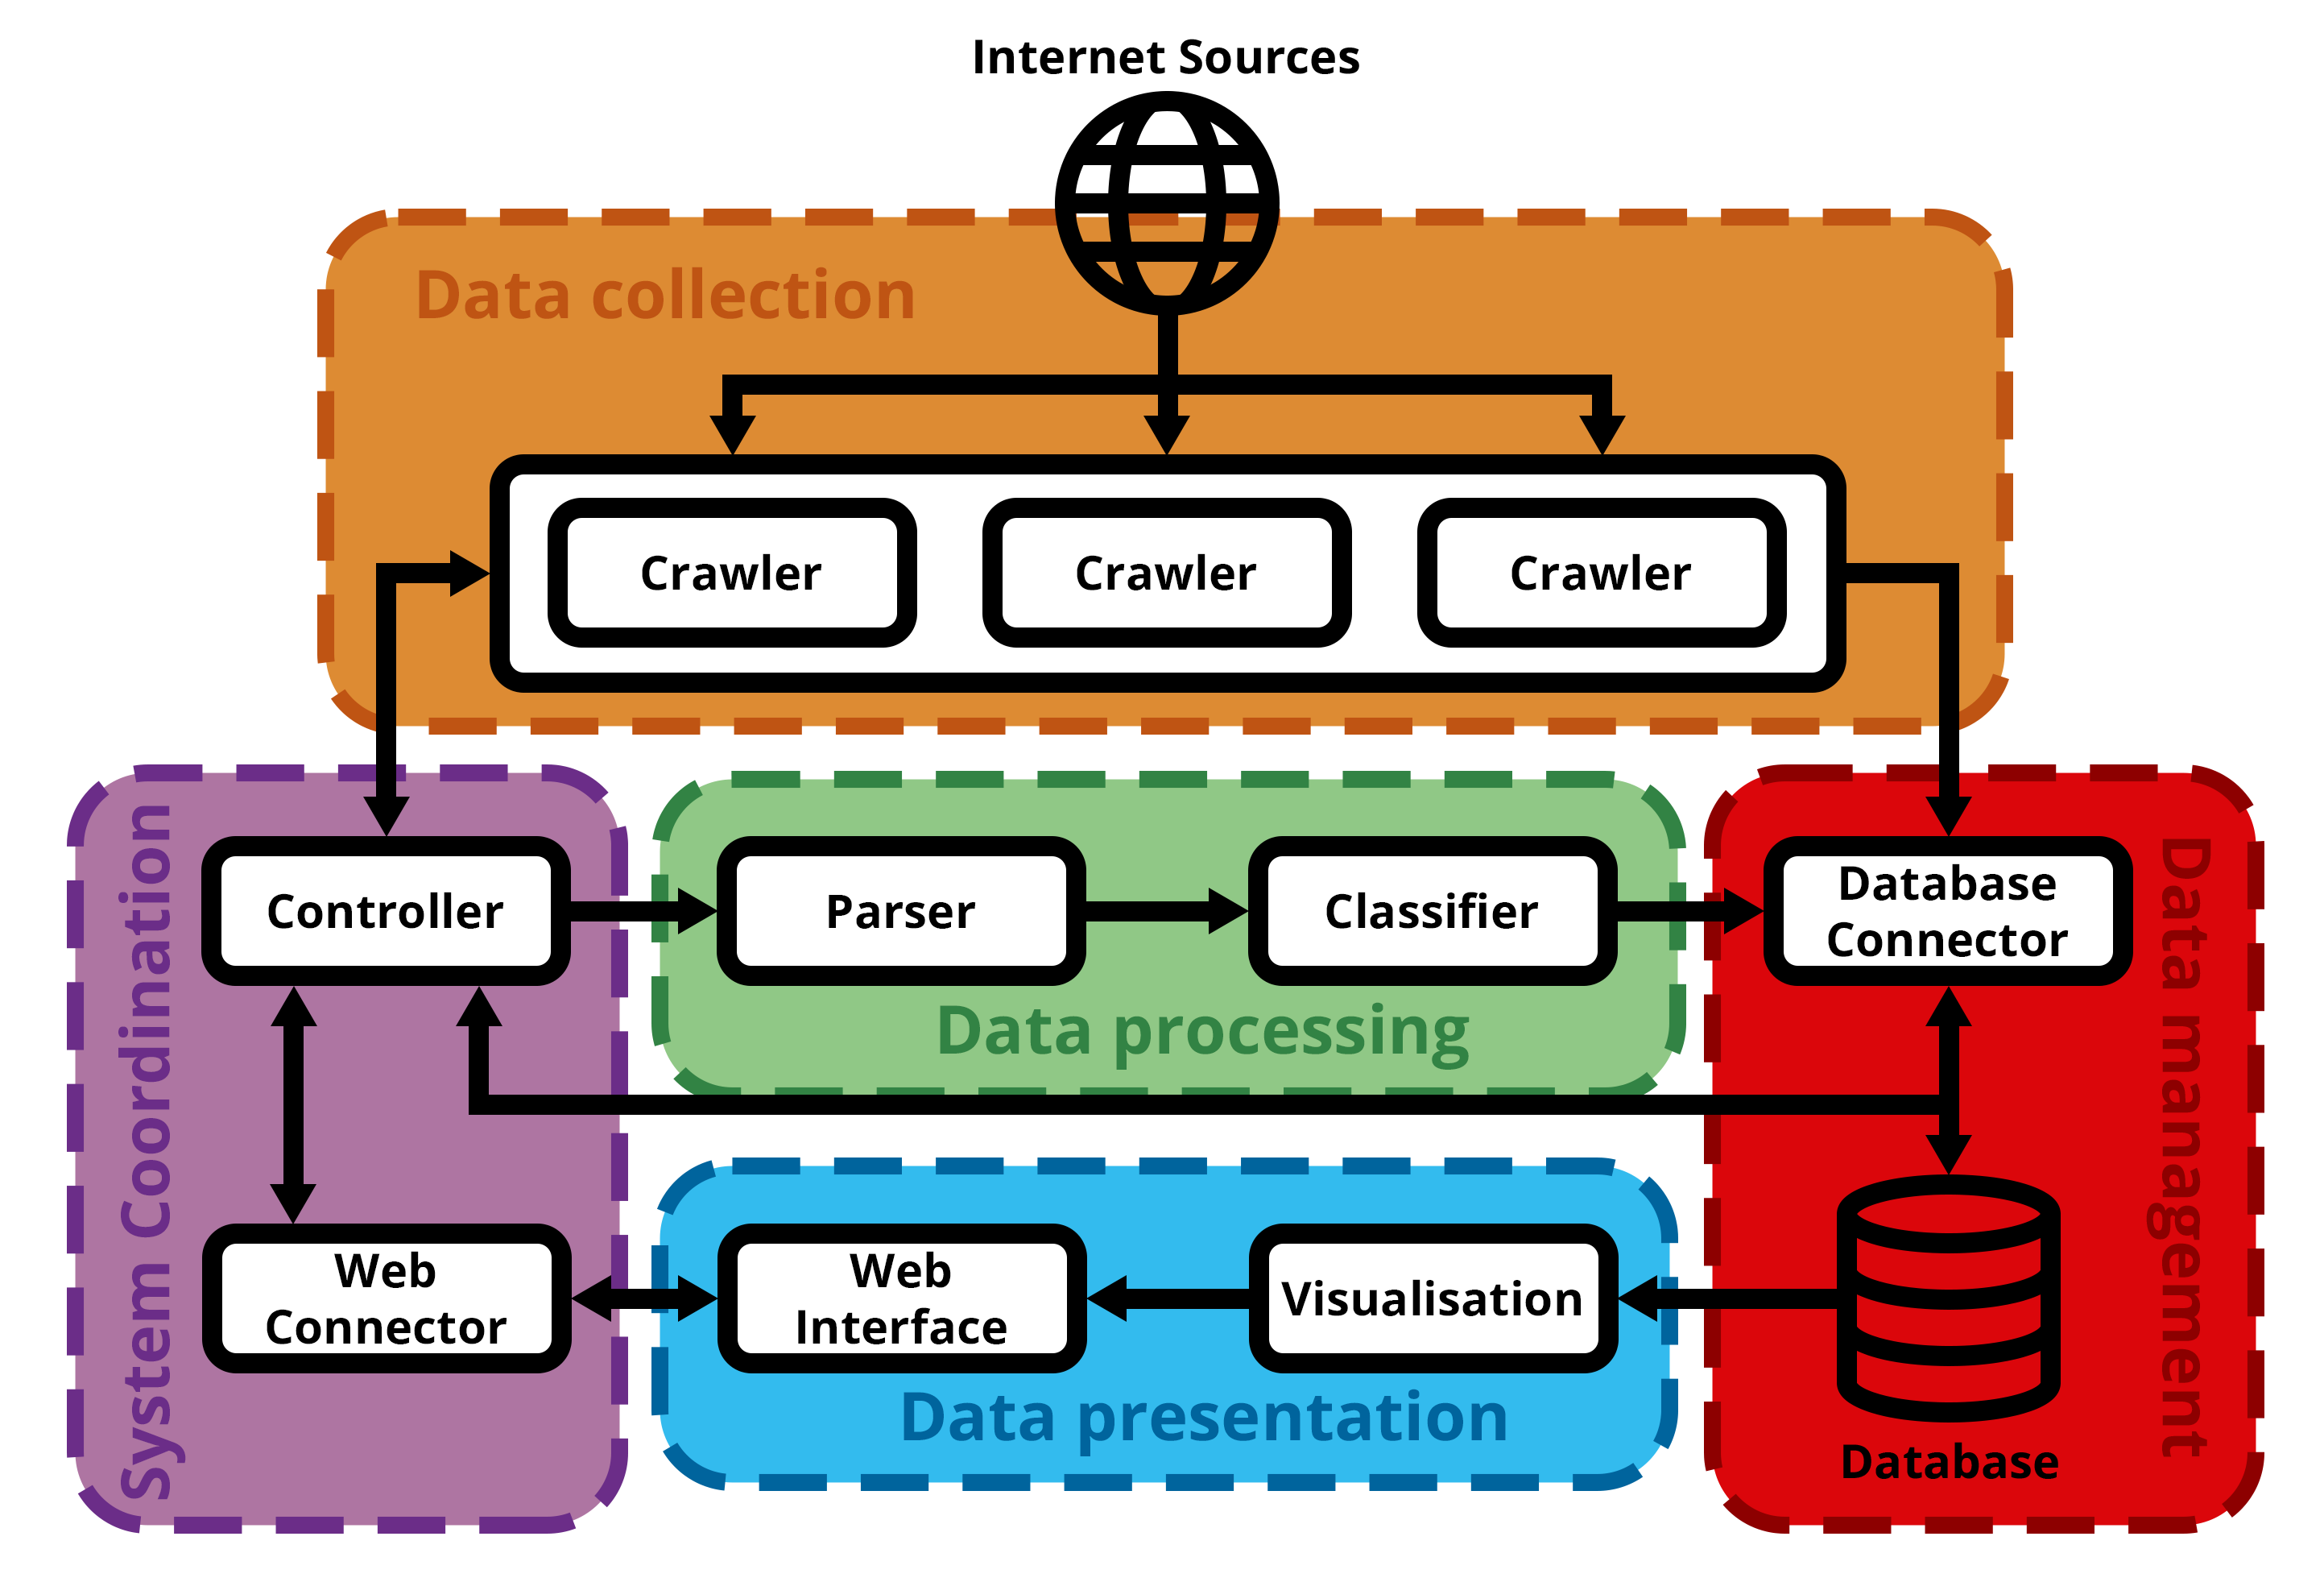
\includegraphics[width=\textwidth]{images/system_overview_diagram.png}
\caption{The overview of the system architecture for this project, showing the different modules and interactions between them. Each module is contained in a box. Arrows indicate the transfer of data between modules (e.g. A -> B means module B receives data from module A. The larger, coloured boxes indicate different subsystems. }
\label{fig:system_overview_diagram}
\end{figure}
\par
\subsection{Modules}
The overall system is designed so that modules can be swapped out and replaced or added into the system in order to cover different sources of online data. In this project, the system and its modules will be designed to gather news articles from RSS feeds and news websites. The purpose of each module in the overall system is as follows:
\begin{itemize}
    \item \textbf{Crawler: } Connect to an internet source (in this case, an RSS feed or website) and obtain a list of URL's to be parsed for the system (in this case URLs of news articles).
    \item \textbf{Article parser: } Parse the given list of URLs, mining the page source content for details (in this case, Headline, publish date etc.)
    \item \textbf{Classifier: } Pass each article through a machine learning model in order to assign it a category (in this case, each news article is given a topic).
    \item \textbf{Database connector: } Provide an interface to allow the system to access the external database.
    \item \textbf{Database: } Permanently store the collected and classified data, and the crawlers, in a structured form.
    \item \textbf{Visualisation: } Present the collected and aggregated data in a number of graphs, charts and statistics for monitoring and interpretation
    \item \textbf{Web interface: } Allow administrators to see the visualisation and to manage the active crawlers.
    \item \textbf{Web connector: } Provide an interface for communication between the management website and the scraping system.
    \item \textbf{Controller: } Initialise crawlers from the sources stored in the database. Send the parsed articles to the classifier and communicate with the web interface (send updates and receive instructions).
\end{itemize}


\section{Data Collection}
The data collection system crawls an internet source for all URLs which can possibly contain useful information. In this project, we are concerned with finding the URLs of news articles from a news website or RSS feed. To be appropriate in a disease surveillance system, the data should be updated in near real-time so outbreaks can be quickly understood and responded to.

\subsection{Crawler}
The crawler is the first stage of the data collection process. It represents one individual data source collected in the system, either an RSS feed or a website which is scraped for articles. Crawler objects are stored as a row in a data table of sources. The objects are instantiated from information given by the web interface when a new source is added, or from an existing source in the database. The responsibilities of a crawler are:
\begin{itemize}
    \item Instantiate itself from information stored in the database or given by the web interface.
    \item Add itself to the database if it did not already exist.
    \item Establish a connection with an internet source, in order to receive information.
    \item Create a list of potential sources of data to be parsed (a list of article URLs).
    \item Update its state when it has received new data or instructions.
    \item Update the database with its new state (e.g. delete itself or update its last scrape time).
\end{itemize}
An abstract crawler class encapsulates most of the functionality of this module, handling all communication between other modules. Any concrete crawler implementations (in this project, there are 2: RSS feed crawler and Web crawler) only have to create a method to crawl specific types of data from the internet and use it to update the last scraped date, as well as override the constructor to add its source type. A full diagram of crawler functionality is shown in Figure \ref{fig:crawler_diagram}
 \begin{figure}[h]
\centering
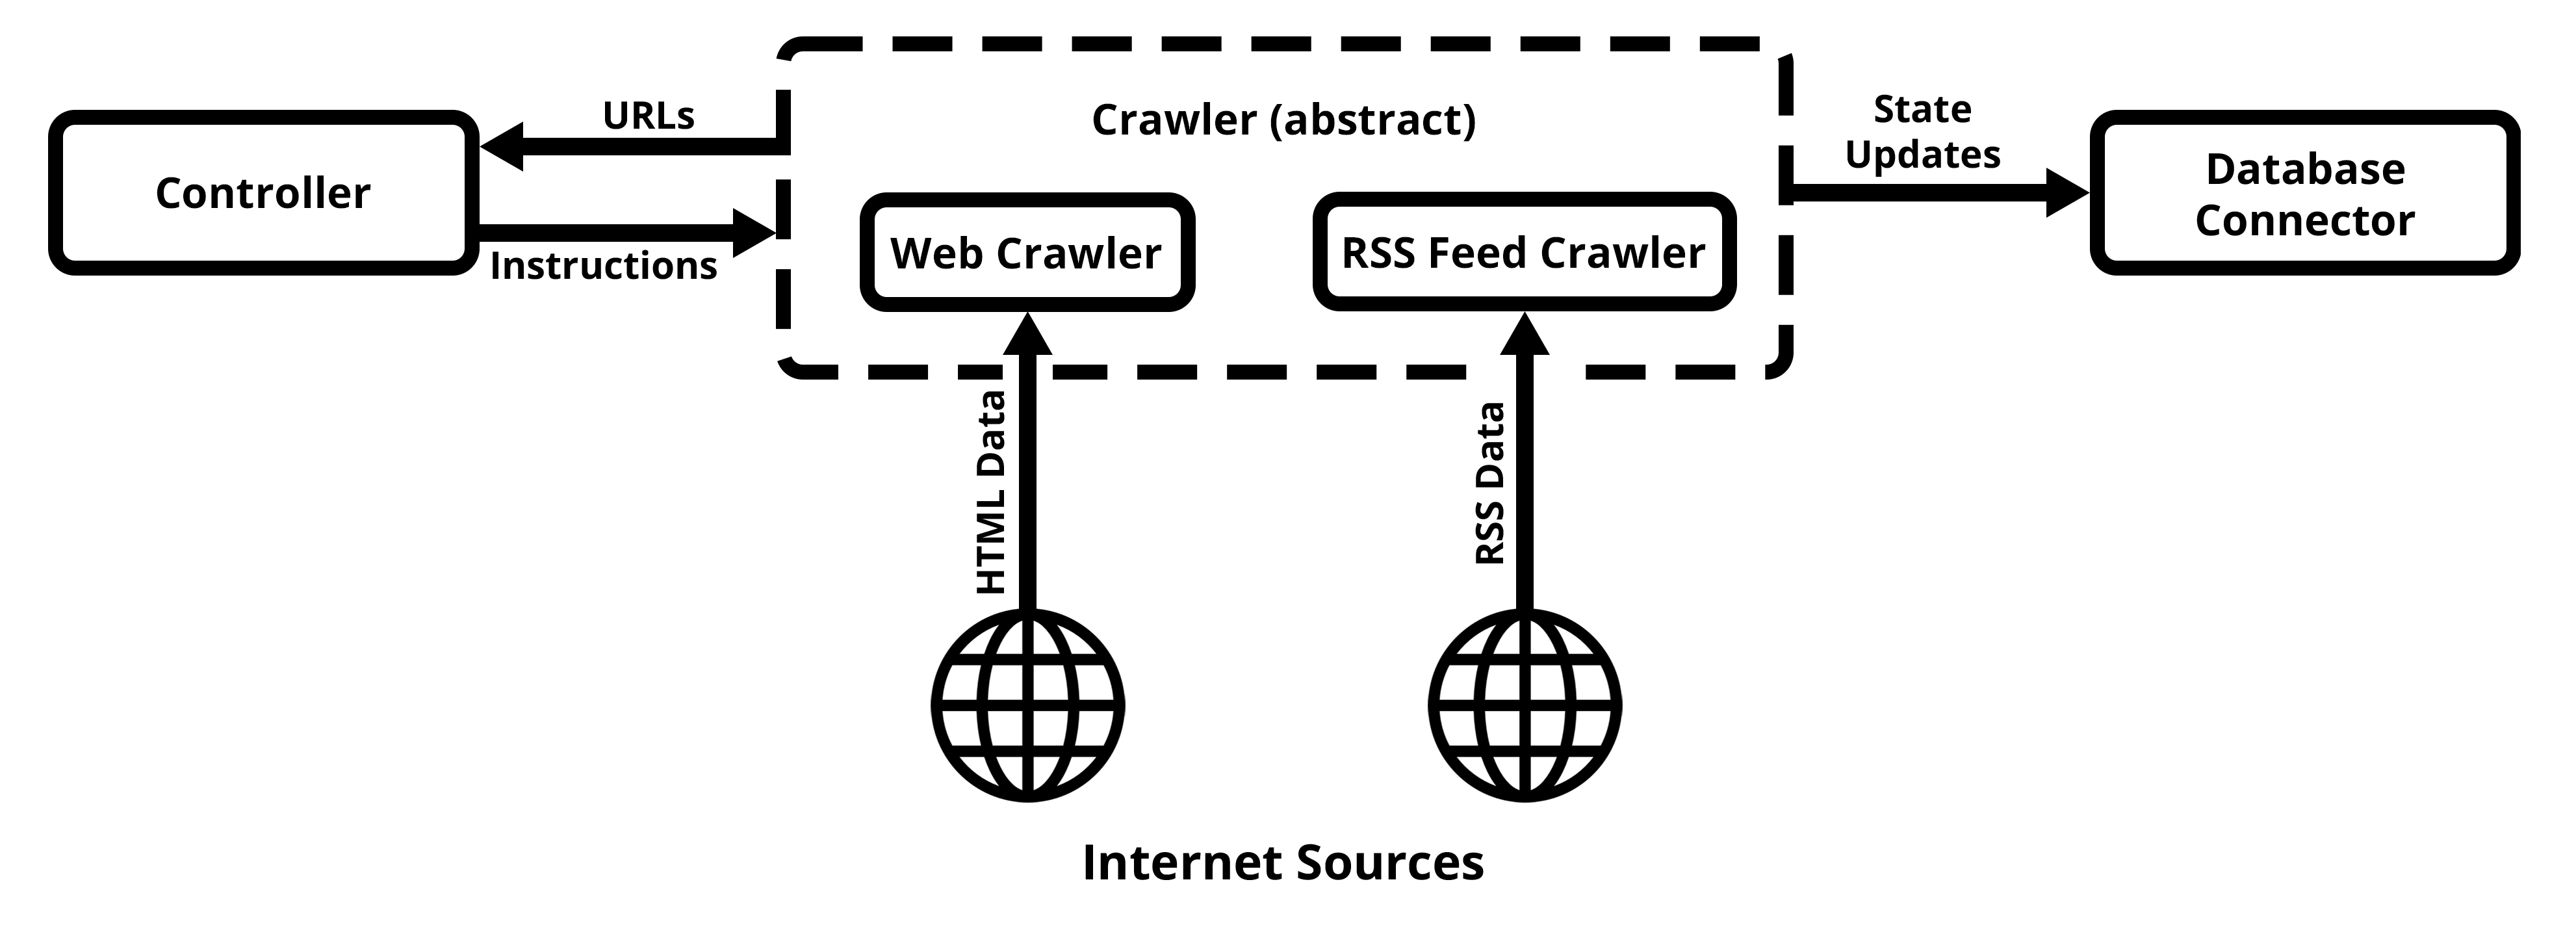
\includegraphics[width=\textwidth]{images/Crawler-diagram.png}
\caption{The overview of the inputs and outputs of the crawler system. The diagram shows the concrete Web Crawler and RSS Feed Crawler implementations being encapsulated by the abstract crawler class, which handles interactions with other modules. The concrete classes each collect a different type of data from the internet sources.}
\label{fig:crawler_diagram}
\end{figure}


\section{Data Processing}
The data processing system creates structured data from internet sources, converting unclean data such as an RSS feed or the HTML of a webpage into a formatted news article with a headline and article body and associated data. It also attempts to understand the data by assigning a category to the incoming articles. The data processing subsystem should be able to process data at a high volume from sources in 10 different languages: English, French, Spanish, Portuguese, Russian, Indonesian, Mandarin, Korean and Arabic. When data is processed, it will be added to the database so it can be used in visualisation.

\subsection{Parser}
The parser receives as input a combined list of URLs from the crawlers and for each URL, will retrieve the page HTML and use it to extract details about the page (in this case, the pages will be news articles) which can be inserted into the database. The article URLs will be shuffled randomly before parsing to avoid very fast repeated requests to the same host, which smaller sources may not be able to easily handle. The parser assumes that news sources are monolingual to avoid language detection wherever possible, but will attempt to detect the language if parsing is incorrect. After this process is complete, the parser sends the parsed data to the classifier to assign the article a topic. The information required from a news article for this project, which the parser will attempt to scrape, is:
\begin{itemize}
    \item Article headline
    \item Article body
    \item Publish date
    \item Language
\end{itemize}
 An abstract parser class handles all communication with other modules. Any concrete parser implementations (such as the article parser in this project) only have to implement a specific method for crawling a list of given URLs and retrieving structured data from the URLs and returning a final list. A full diagram of parser functionality is shown in Figure \ref{fig:parser_diagram}
 \begin{figure}[h]
\centering
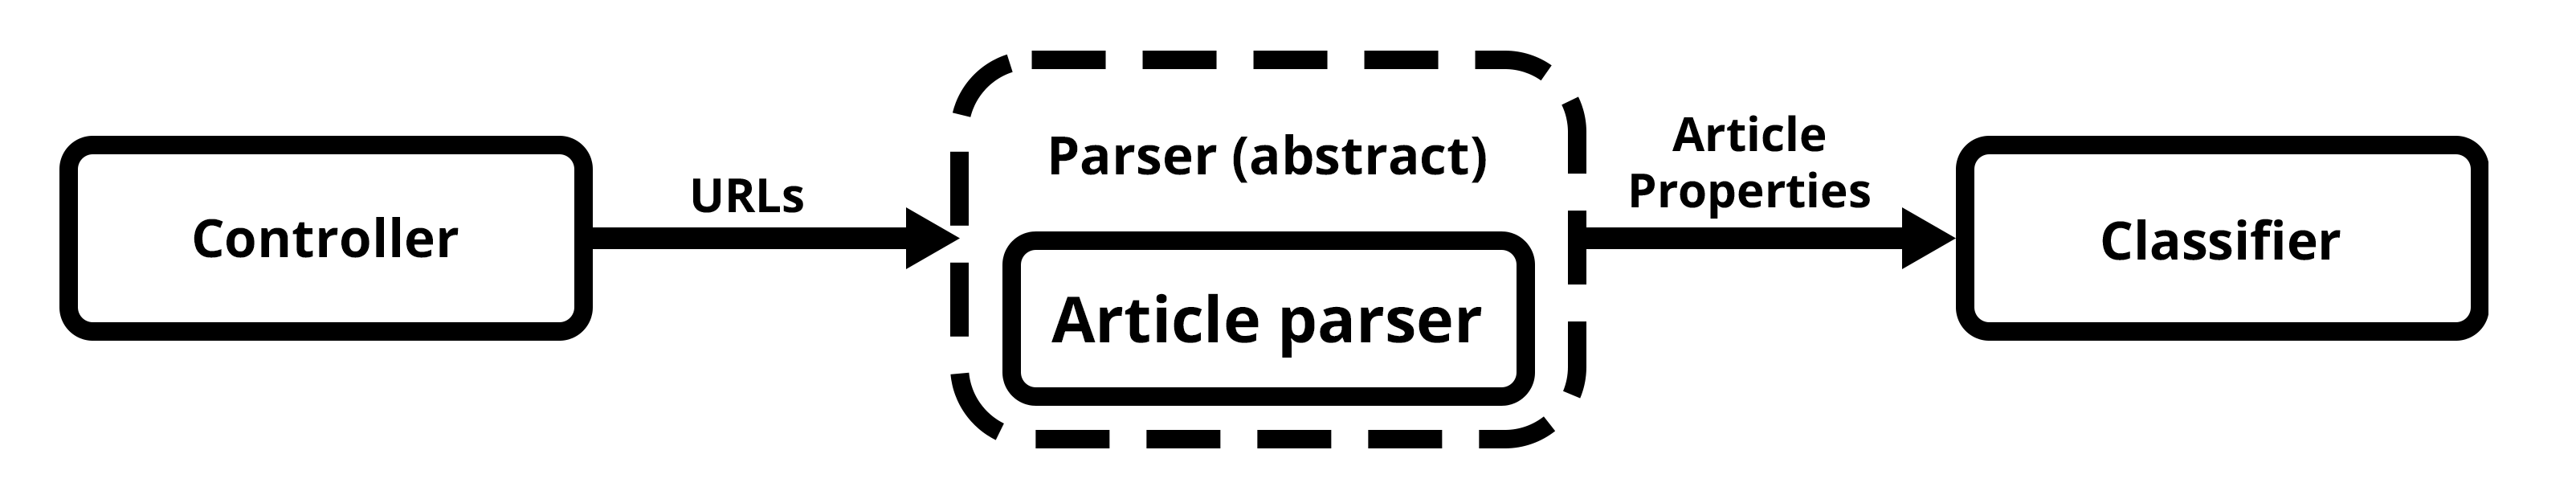
\includegraphics[width=\textwidth]{images/Parser-diagram.png}
\caption{The overview of the inputs and outputs of the parser system. The diagram shows the concrete article parser implementation being encapsulated by the abstract parser class, which handles interactions with the controller and classifier.}
\label{fig:parser_diagram}
\end{figure}

\subsection{Classifier}
The classifier receives a list of parsed articles, with features extracted. It then performs any necessary data preparations and tokenization before feeding the articles through a trained classifier model to assign a category to each news article (e.g. Sports, Entertainment). In this project, the classifier module will use a pre-trained BERT-based classifier model loaded from a file and will tokenize and classify the concatenated article headline and body. The parsed articles with topics will be sent to the database connector and inserted into the database. \par
An abstract classifier class handles communication with other modules and batching of input data. To create a concrete classifier implementation, we would have to implement:
\begin{itemize}
    \item A constructor which properly initialises the model and any tokenizers.
    \item A method which preprocesses a list of input data.
    \item A method which receives an input batch and outputs a list of corresponding classification labels.
\end{itemize}

A full diagram of classifier functionality is shown in Figure \ref{fig:classifier_diagram}

 \begin{figure}[h]
\centering
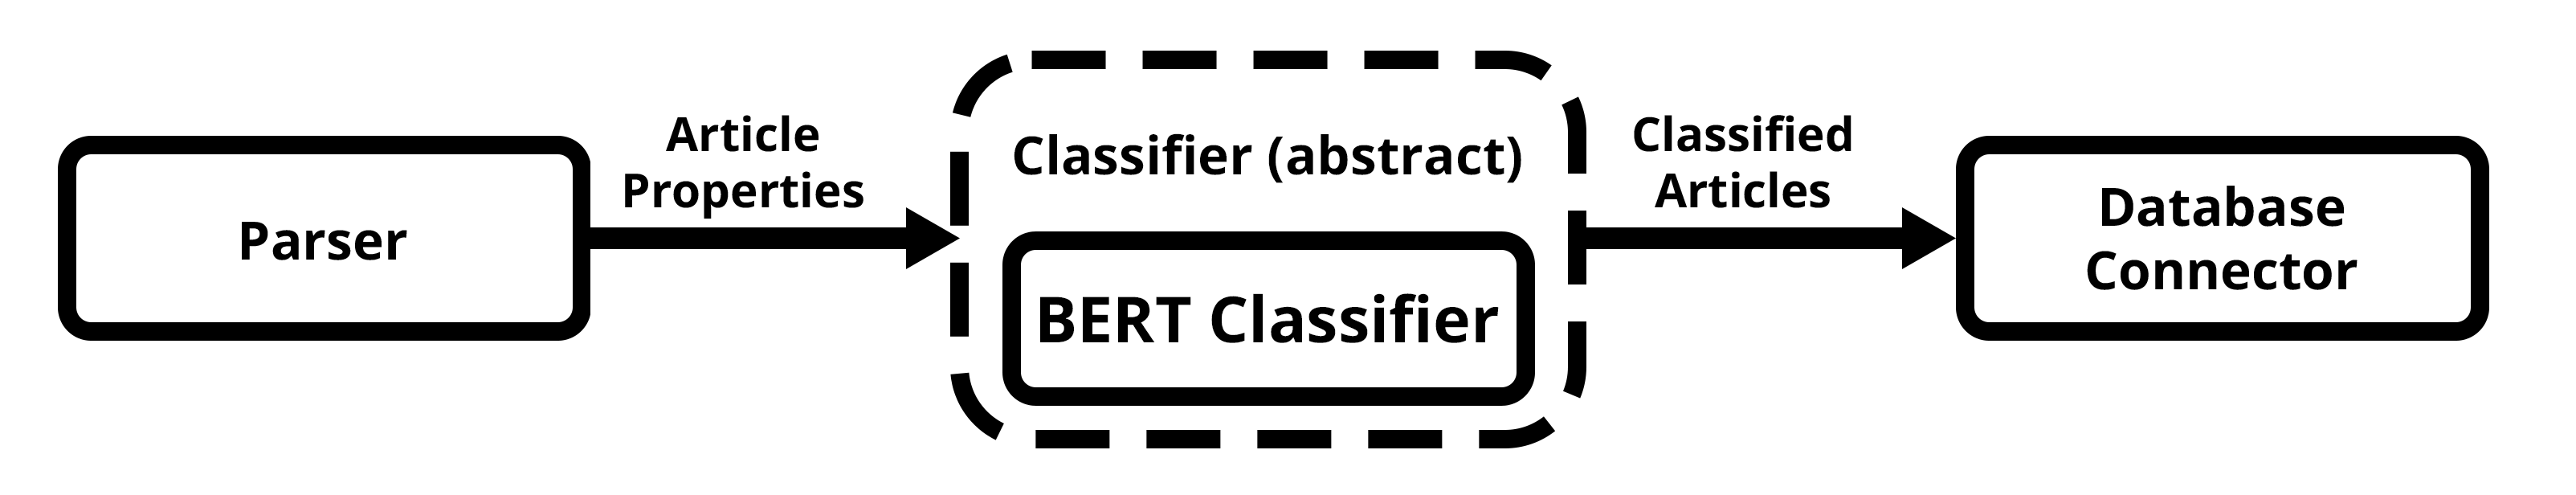
\includegraphics[width=\textwidth]{images/Classifier-diagram.png}
\caption{The overview of the inputs and outputs of the classifier system. The diagram shows the concrete BERT classifier implementation being encapsulated by the abstract classifier, which handles interactions with the parser and database connector.}
\label{fig:classifier_diagram}
\end{figure}

\section{Data Management}
The data management subsystem stores the data (data sources and collected articles) in a permanent form, where it can be shown in the visualisations. The database system should be able to handle many reads (for article duplicate checking) and writes (for inserting new articles) at a high volume. 

\subsection{Database}
For this project, the database will consist of two tables: \textbf{Articles} and \textbf{Sources}. The attributes for these tables are shown in Table \ref{table:schema}

\begin{table}[h]
\begin{tabular}{lll}
\hline
\multicolumn{3}{c}{\textbf{Source}}                                                                                                                                      \\ \hline
\textbf{Attribute} & \textbf{Type} & \textbf{Description}                                                                                                                \\ \hline
\textbf{ID}        & Primary Key   & A unique auto-generated source ID.                                                                                                  \\
URL                & Text          & The data source URL (e.g. "https://www.bbc.co.uk/news")                                                                             \\
Name               & Text          & A name describing the source (e.g. "BBC News")                                                                                      \\
Country            & Text (2)      & \begin{tabular}[c]{@{}l@{}}The ISO 3166-1 alpha-2\tablefootnote{https://en.wikipedia.org/wiki/ISO\_3166-1\_alpha-2} code of the country \\ the source originates from (e.g. "GB")\end{tabular}        \\
Language           & Text (2)      & The ISO 639-1\tablefootnote{https://en.wikipedia.org/wiki/List\_of\_ISO\_639-1\_codes} code of the sources main language (e.g. "EN")                                                                         \\
Data Source        & Text          & The type of source this is (e.g. "RSS/Atom feed")                                                                                   \\
Last retrieved     & Date/Time     & The time this source last retrieved new data                                                                                        \\
Active             & Boolean       & \begin{tabular}[c]{@{}l@{}}Whether this source is active \\ (if False, when instantiated the crawler will be disabled)\end{tabular} \\ \hline
\multicolumn{3}{c}{\textbf{Article}}                                                                                                                                     \\ \hline
\textbf{Attribute} & \textbf{Type} & \textbf{Description}                                                                                                                \\ \hline
\textbf{ID}        & Primary Key   & A unique auto-generated article ID.                                                                                                 \\
URL                & Text          & The URL of the article                                                                                                              \\
Headline           & Text          & The article headline                                                                                                                \\
Body               & Text          & The main body of the article                                                                                                        \\
Country            & Text (2)      & The ISO 3166-1 code of the country of the original source                                                                           \\
Language           & Text (2)      & The ISO 639-1 code of the language of the article                                                                                   \\
Published          & Date/Time     & The time this article was published                                                                                                 \\
Retrieved          & Date/Time     & The time this article was retrieved by the scraping system                                                                          \\
Source name        & Text          & The name of the source this article is collected from                                                                               \\
Source type        & Text          & The type of source this article came from (e.g. "Web scraper")                                                                      \\
Category           & Text          & The assigned category of this article (e.g. "Entertainment")                                                                        \\ \hline
\end{tabular}
\caption{List of attributes in the Source and Article tables, with data type and description. Primary key attributes are highlighted in bold. "Text (2)" denotes that this field is a text field which is exactly 2 characters long.}
\label{table:schema}
\end{table}

\subsection{Database Connector}
The database connector provides a connection between the system and the external database, allowing the other modules to send and retrieve the data. In this system, the connector must have functionality for:
\begin{itemize}
    \item Creating the Article and Source tables
    \item Adding new sources and articles
    \item Retrieving stored sources
    \item Deleting sources
    \item Updating sources (enabling/disabling, updating last scrape time)
    \item Searching articles by URL and headline (for duplicate checking) 
\end{itemize}
A full diagram of database functionality is shown in Figure \ref{fig:database_diagram}
 \begin{figure}[h]
\centering
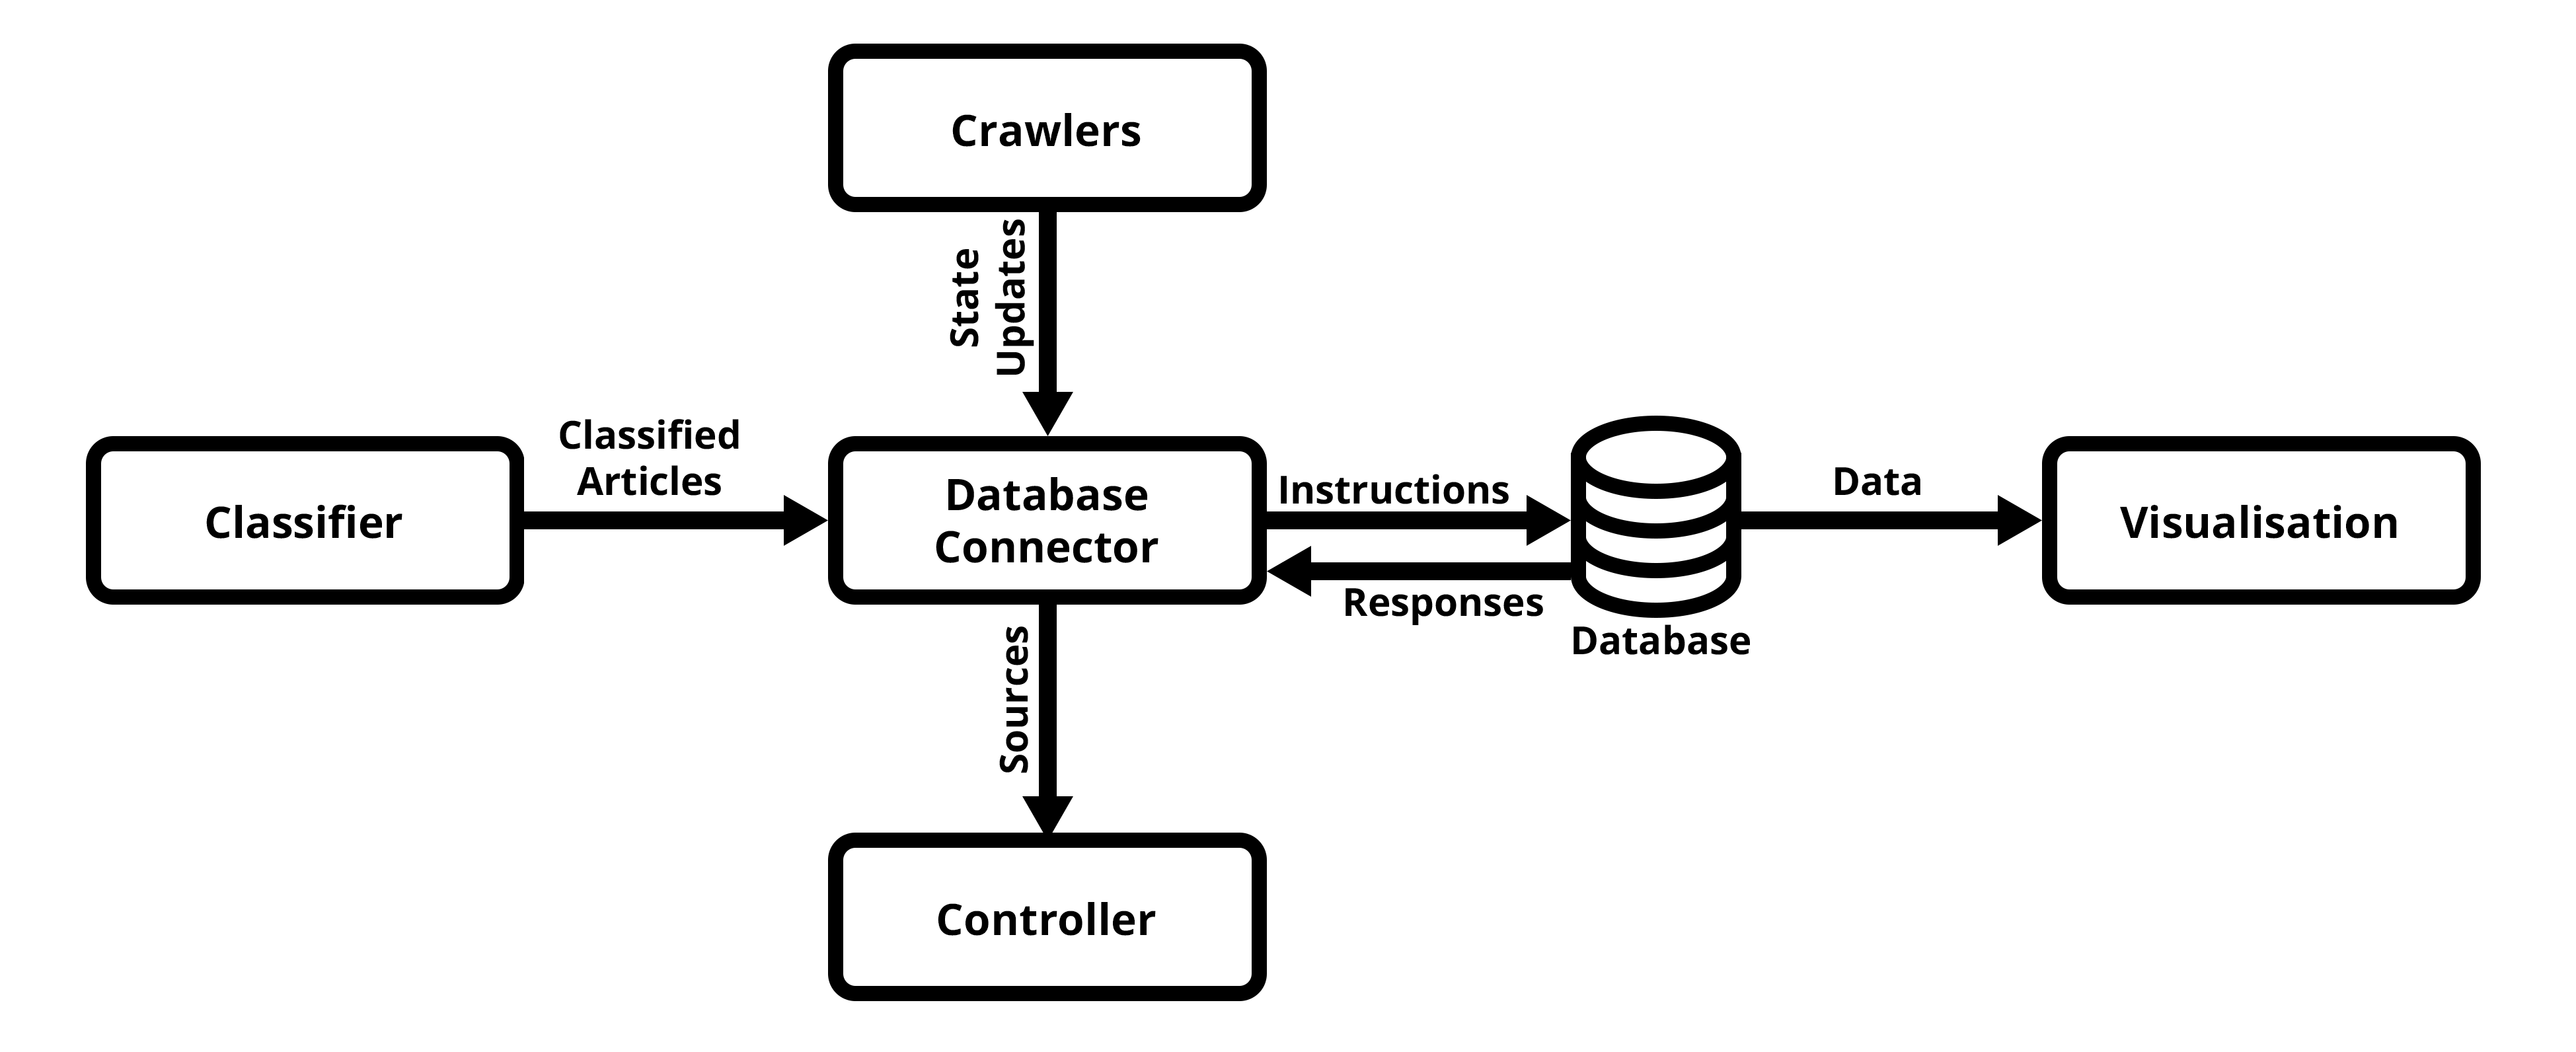
\includegraphics[width=\textwidth]{images/Database-diagram.png}
\caption{The overview of the inputs and outputs of the database and connector.}
\label{fig:database_diagram}
\end{figure}
\section{Data Presentation}
The data presentation subsystem is concerned with creating an easy interface for a user to view, analyse and understand the data collected, as well as easily interact with the system to modify its behaviour. The system should have interfaces which are easy to use and understand and provide useful insight and control on the data collection process.

\subsection{Visualisation}
The visualisation is mainly based on the current BioCaster interface, as shown in Figure \ref{fig:biocaster_visualisation}. This design has been updated to reflect the changes from my project to the current system, including the addition of news article topics and different source types of information retrieved. I also did not have the specific region or disease information to create the alerts seen on the BioCaster interface. Shown in Figure \ref{fig:visualisation-wireframe} is an initial wireframe of the new visualisation: \par
 \begin{figure}[h]
\centering
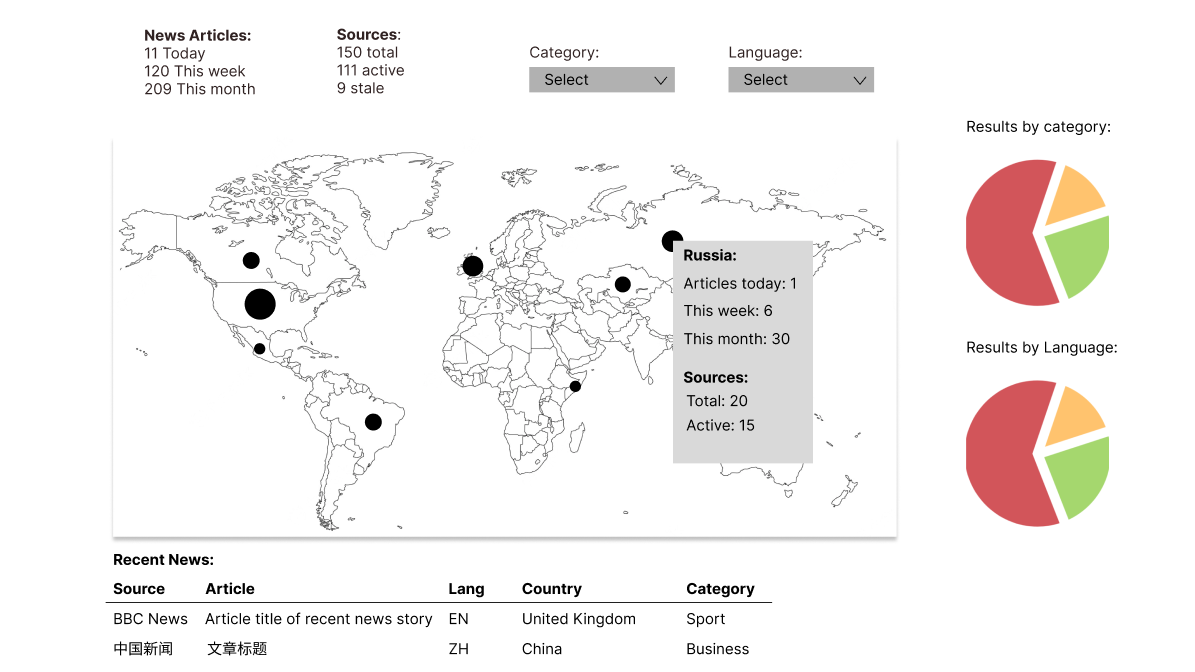
\includegraphics[width=\textwidth]{images/visualisation-wireframe.png}
\caption{The wireframe for the new visualisation.}
\label{fig:visualisation-wireframe}
\end{figure}
After supervisor feedback, more emphasis was placed on filtering by source type. The final visualisation will have the following modules:
\begin{itemize}
    \item A bar for filtering by Category, Language and Source type
    \item A section showing the number of total and active sources
    \item A section showing the number of articles scraped today, this week and this month
    \item Pie charts showing data distribution by source type, language and category
    \item A table showing the most recent articles collected
    \item Time-series data on articles collected over time
    \item A world map showing information per country (number of articles, most common category etc.)
\end{itemize}

\subsection{Web Interface}
The web interface is designed to show the visualisation on a webpage, as well as provide functionality for managing the scraping system. The web interface should provide utility for the following tasks:
\begin{itemize}
    \item Enabling/disabling the entire scraping system
    \item Enabling/disabling individual sources
    \item Deleting individual sources
    \item Adding new sources
    \item Viewing stale sources (this was requested by a member of the BioCaster team in a meeting)
\end{itemize}
The wireframe for the manage sources page of the web interface is shown in Figure \ref{fig:interface-wireframe} 
 \begin{figure}[h]
\centering
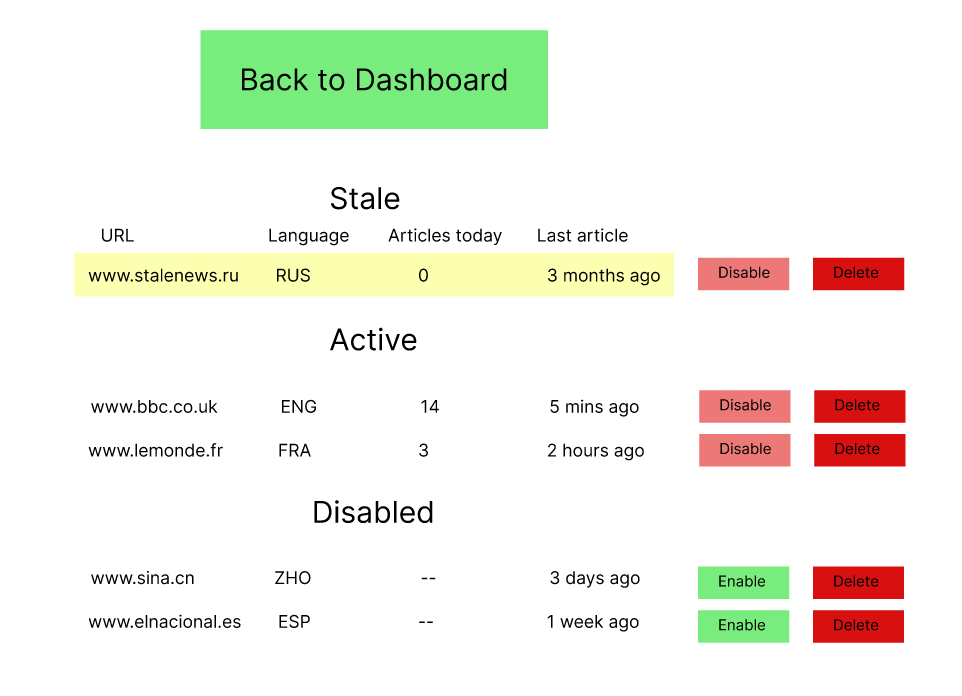
\includegraphics[width=\textwidth]{images/interface-wireframe-sources.png}
\caption{The wireframe for the manage sources page of the web interface.}
\label{fig:interface-wireframe}
\end{figure}

\section{System Coordination}
The system coordination subsystem is responsible for orchestrating the data collection process and connecting subsystems, as well as allowing the interface to communicate with the scraping system.
\subsection{Web Connector}
The web connector provides the interface between the web server and the scraping system. It ensures that the commands performed on the interface are translated into instructions for the controller, which will perform the requested action. These instructions include enabling, disabling, deleting and adding sources, as well as enabling or disabling the entire scraping system. The web interface can also request updates through the web connector, to show the user the most recent information on the most recent scrape times of each source. Figure \ref{web-connector-diagram} shows how the web connector integrates with all other modules.
 \begin{figure}[h]
\centering

\includegraphics[width=\textwidth]{images/Web-connector-diagram.png}
\caption{The overview of the inputs and outputs of the web connector.}
\label{fig:web-connector-diagram}
\end{figure}

\subsection{Controller}
The controller is responsible for the coordination of the system and is the module called to run the system. It performs the following roles:
\begin{itemize}
    \item Ensures the tables exist in the database.
    \item Receives all sources from the database and instantiates crawlers.
    \item Instantiates parser and classifier object(s).
    \item Builds the pipelines for data collection and processing.
    \item Starts the web server for the web interface.
    \item Controls when the crawlers look for new data.
    \item Sends new crawler data to the parser(s).
    \item Communicates with the web interface through the web connector, sending updates and performing instructions.
\end{itemize}
A full diagram of the controller functionality is shown in Figure \ref{fig:controller_diagram}.
 \begin{figure}[h]
\centering
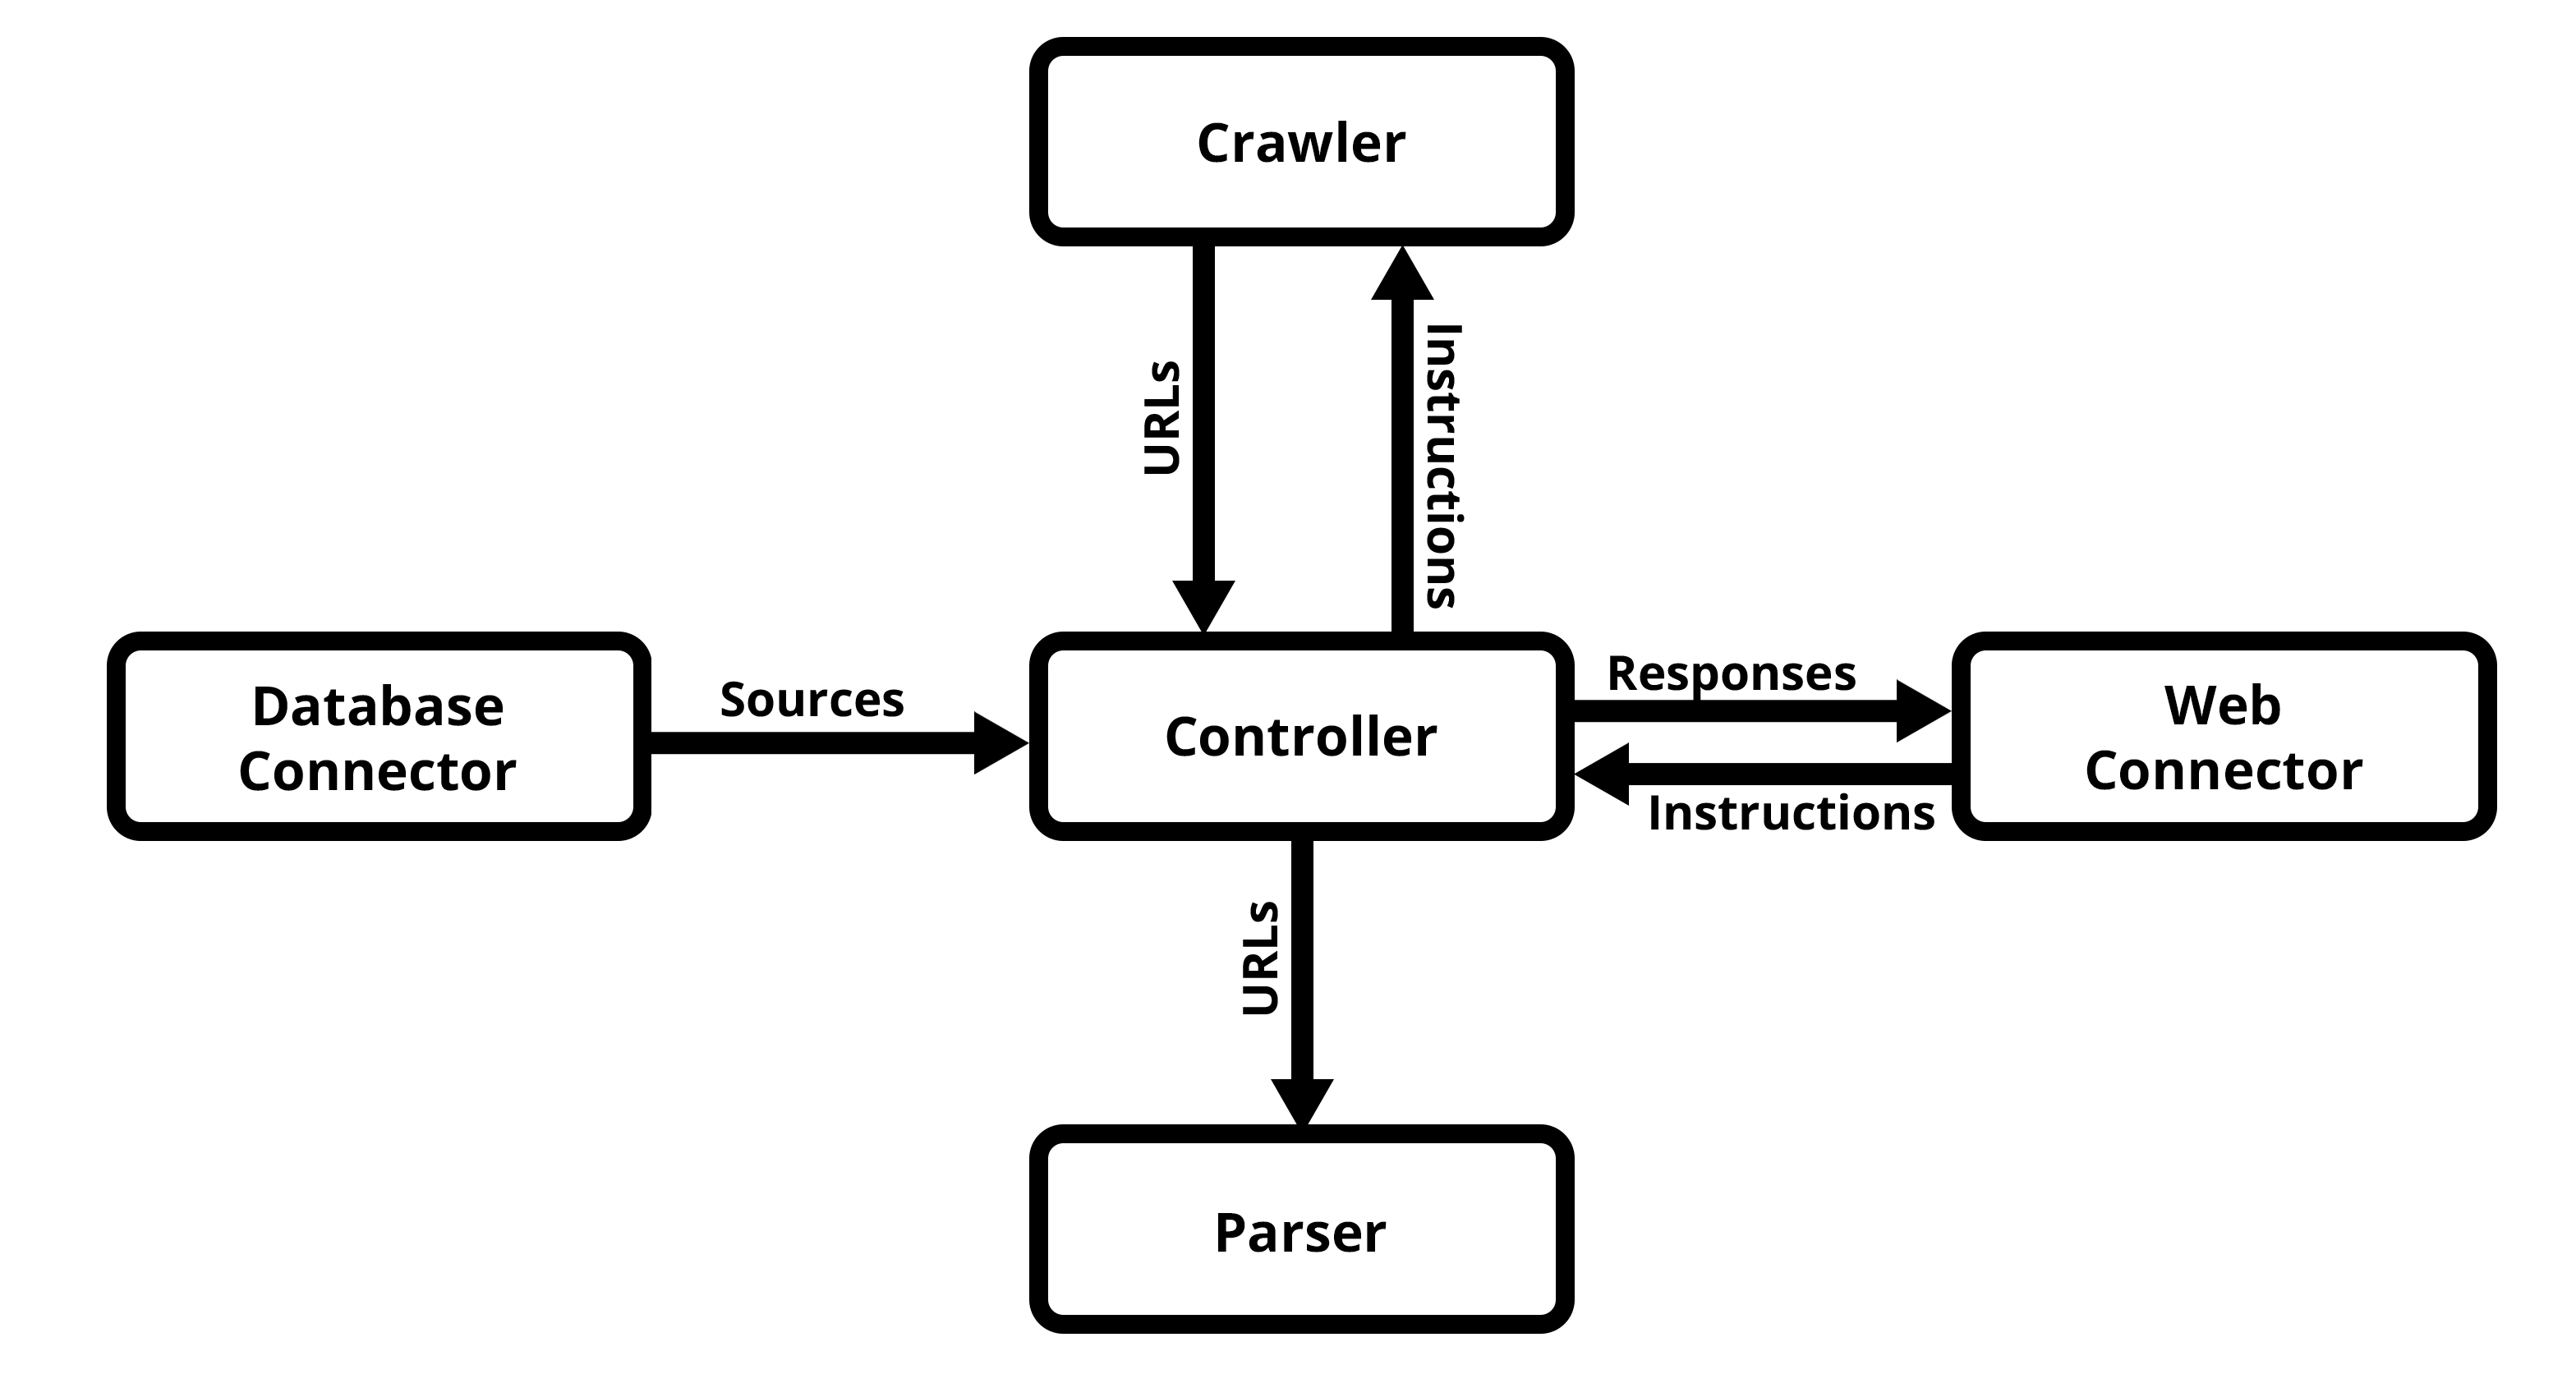
\includegraphics[width=\textwidth]{images/Controller-diagram.png}
\caption{The overview of the inputs and outputs of the controller module.}
\label{fig:controller_diagram}
\end{figure}

%==================================================================================================================================


\chapter{Implementation}
This section describes the implementation of each of the previously described sections, including details of the algorithms, libraries and technologies used. The system is written in Python as this is a very common language, especially for machine learning programs, and has many libraries available for web crawling, web scraping and database communication.

\section{Crawlers}
Generally, the purpose of the crawler is to return a list of URLs for parsing given a source URL. The crawlers also control the updating of their own state in the database. The implementation of this functionality is shown below in Figure \ref{fig:abstract-crawler}.
\subsection{Instantiation}
Concrete implementations of crawlers will extend the constructor of the abstract crawler, by adding their source type as a parameter and possibly in other ways. The abstract crawler handles the consistent details of instantiation, as listed below:
\begin{itemize}
    \item Initialise URL, and "is enabled" variables (crawlers are enabled by default)
    \item Initialise language, if given
    \item Initialise source ID if given, otherwise create the source object in the database and initialise the new source ID returned by the operation
    \item Initialise country if given (using a dictionary of country names to ISO 3166 alpha-2 code if necessary), otherwise attempt to mine it from the URL (e.g. .co.uk website implies "GB")
    \item Initialise the last scrape time if it exists, otherwise set it to a default value
\end{itemize}
The abstract crawler also includes all functions which interface with the database connector, using its source ID: Update last scrape time to a given time (if it is more recent than the current time), enable/disable and delete. These functions are called in response to commands from the web interface. If specified in the config, a scraper can automatically disable itself if it is stale. The main "crawl" method which is called by the connector will retrieve a list of new articles using a method overridden by a concrete implementation, and then return all non-duplicate URLs (checked by searching for each of the URLs in the database) packaged with the language, country, source name, source type and a reference to itself so that the parser can update the crawlers last scrape time when it finds the date of an article.

\subsection{Web Crawler}
To retrieve new articles, the web crawler uses the \emph{Newspaper3K}\footnote{https://github.com/codelucas/newspaper} library to create an object which scrapes the whole website of a given URL. It is designed to be fed the homepage URL of a news site, and creates an object which crawls the pages for all available links to news articles, stored in the "articles" property. The web crawler returns all of these articles which do not contain special URL characters ? or \# (to prevent duplicate articles).
\subsection{RSS/Atom Feed Crawler}
RSS Feed entries are collected using the \emph{feedparser}\footnote{https://pypi.org/project/feedparser/} library which given a URL to an RSS or Atom feed will create a dictionary representing all of the RSS feed data. The crawler will iterate through each feed entry, and for any published after the most recent scrape date of the crawler will return the article URL. If no dates are attached, the crawler will return all articles from the feed. \par
If not supplied a country, the feed crawler will attempt to determine the language from a "language" property in the RSS feed. If this property does not exist, the crawler will use the \emph{langdetect}\footnote{https://pypi.org/project/langdetect/} library to attempt to detect the language of the headline of the first entry. This library uses the Google translate API to return a predicted language for a given text input. If it cannot detect the language, it will set the language to unknown.


\section{Parser}
The parser module will receive a combined list of all of the new URLs obtained from each crawler. It will retrieve the details (title, body and publish date) of each given item using a method defined in a concrete implementation, and update each crawler with the new most recent article retrieval date. It will then pass the parsed results to the classifier module.
\subsection{Instantiation}
The abstract parser is instantiated with two arguments: A classifier, which parsed articles will be passed to, and a lock, which is used to reserve access to the crawler objects while their most recent scrape times are being updated, to avoid inconsistent updates from multiple sources at the same time which may lead to some of the operations not taking effect. The parser also retrieves a minimum article length from the config, to ensure that articles which do not contain enough content are filtered out.
\subsection{Article Parser}

\subsubsection{Choice of library} \hfill \par
The main free and open-source technologies for scraping news articles from websites in Python were \emph{Newspaper3K}\footnote{https://github.com/codelucas/newspaper} and \emph{news-please}\footnote{https://github.com/fhamborg/news-please}, which is built on top of Newspaper3K and adds some extra features. Another option considered was \emph{Newscatcher}\footnote{https://newscatcherapi.com/news-api}, but the free API is limited in how many calls can be made and this made it unsuitable for this project. Finally, we considered \emph{pygooglenews}\footnote{https://github.com/kotartemiy/pygooglenews} which provided some promise in using google news to find articles under certain subjects, keywords, languages and regions. For this project, I found it desirable to have better control of the exact sources collected, instead of filtering through keywords and relying on Google's source selection, but a scraper using this library could easily be added to extend the capabilities of the current system. We decided to move forward with the former two libraries and conducted an experiment to compare their capabilities. \par

We compared the features present in each of the two libraries. Notably, Newspaper3K can perform full website scraping in Python, whereas news-please can only do this using its Command Line Interface (CLI). We attempted to scrape 3 articles from each of 109 previously selected websites, across 10 languages (English, French, Spanish, Portuguese, Russian, Indonesian, Mandarin, Korean and Arabic), and compared the number of successful scrapes (without error) and the average speed. The results are shown in Table \ref{table:scraper-library-results}. \par 

\begin{table}[]
\begin{tabular}{llllll}
\hline
\textbf{Language}   & \textbf{No. Sources} & \multicolumn{2}{l}{\textbf{Newspaper3K}}                 & \multicolumn{2}{l}{\textbf{news-please}}                 \\ \cline{3-6} 
\textbf{}           & \textbf{}            & \textbf{No. Correct} & \textbf{Average time (ms)} & \textbf{No. Correct} & \textbf{Average time (ms)} \\ \hline
\textbf{English}    & 28                   & \textbf{28}          & \textbf{536.3332}                 & 26                   & 704.3305                          \\
\textbf{French}     & 11                   & 11                   & 1548.167                          & 11                   & \textbf{806.2918}                 \\
\textbf{Spanish}    & 10                   & 9                    & \textbf{339.2322}                 & 9                    & 435.0289                          \\
\textbf{Mandarin}   & 9                    & 8                    & 3538.55                           & \textbf{9}           & \textbf{3137.15}                  \\
\textbf{Russian}    & 9                    & 8                    & \textbf{632.5125}                 & 8                    & 755.09                            \\
\textbf{Portuguese} & 10                   & 10                   & \textbf{1220.08}                  & 10                   & 1289.466                          \\
\textbf{Indonesian} & 5                    & 5                    & \textbf{1152.32}                  & 5                    & 1243.918                          \\
\textbf{Swahili}    & 7                    & 6                    & \textbf{874.445}                  & \textbf{7}           & 1253.669                          \\
\textbf{Korean}     & 6                    & 6                    & \textbf{1629.06}                  & 6                    & 1766.223                          \\
\textbf{Arabic}     & 14                   & \textbf{12}          & \textbf{513.9133}                 & 11                   & 651.8164                          \\ \hline
\textbf{Overall}    & 109                  & \textbf{103}         & \textbf{1198.4613}                & 102                  & 1204.2984                         \\ \hline
\end{tabular}
\caption{The results measuring correctness and speed of the two news scraping libraries on 109 sources in 10 languages. For each source, 3 articles were selected and each article was scraped three times. An average of all of these scrapes per language (in ms, to 4 decimal places), as well as the number of sources correctly parsed, is shown in the table. An overall result is shown, including the average scrape time per language and total number of sources correct. Bold indicates the best performing library in correctness (if not tied) and speed.}
\label{table:scraper-library-results}
\end{table}

Newspaper3K scraped 103 of the 109 websites (94.5\%) without error, whereas news-please scraped 102/109 (93.58\%). The average scraping times are similar in both libraries, but Newspaper3K was faster at scraping in 8 of the 10 languages, and average scraping time per article was 14.82\% lower. Newspaper3K also has the added advantage of requiring one less library, as it is already used in the web crawler. Based on these factors, I chose to use Newspaper3K for the scraping system.
\subsubsection{Parsing news articles} \hfill \par
To parse the given list of URLs with extra details, the article parser implements the following algorithm:
\begin{itemize}
    \item Maintain a list of (source, publish date) pairs and currently parsed articles
    \item For each article URL:
    \begin{itemize}
        \item Attempt to download and parse the URL with Newspaper3K, using the article source's main language
        \item Discard the article if it does not exist or have a title
        \item If the article does not have text, attempt to detect the language of the article headline (using the \emph{langdetect} library)
        \item If the detected language is different to the original language, redownload and parse the article in the new language
        \item Discard the article if there is still no text, or if the text is below the minimum article length
        \item If the parsed article has a publish date, create a new (source, publish date) pair with the article source and parsed publish date
        \item Create a parsed article object which includes URL, title, main text, language, country, publish date, original source and original source type
        \item Add the parsed article to the list of parsed articles
        \item If an exception occurs (e.g. a connection error or a forbidden URL), skip the article
    \end{itemize}
    \item For every (source, publish date) pair, update the source with the new publish date (as the source only updates with newer publish dates, we do not have to find the newest update for each source)
    \item Return the list of parsed articles
\end{itemize}

\section{Classifier}
The classifier module will apply a machine learning model to parsed article data, and send the parsed articles and classifications to the database connector to be added to the database. The abstract classifier class provides the basic structure and some common functionality of the classifier module, such as a constructor which initialises the model and tokenizer, input batching and communication with the database. A concrete classifier implementation will have to implement:
\begin{itemize}
    \item A method for initialising the tokenizer (if necessary)
    \item A method for initialising the model
    \item A method for preparing the input articles for classification (extracting the exact input from the article properties)
    \item A method for tokenizing prepared inputs
    \item A method for classifying a tokenized input batch
\end{itemize}

\subsection{BERT Classifier}
The concrete version of the classifier uses the best performing model on collected real-world training data, loading the pre-trained model from a file with path specified in the constructor. 
\subsubsection{Training data collection} \hfill \par
The sources and keywords for real-world training data were decided as discussed in Section 4.2.2. Any category specific RSS feed was scraped by the system, assigning the corresponding category to each data article before adding to the database. For each news website with category specified in URL, a dictionary of URL keyword to category was created from a manually collected list of category-specific URLs, and any website whose URL contained a category keyword in an appropriate place (e.g. \textbf{sports}.sina.com.cn or aljazeera.net/\textbf{arts}). Before parsing, the URLs were filtered into categories using this matching system, and any articles which didn't match were discarded. Any of these articles which could correctly parse were added to the database with their corresponding category. This process continued until enough articles (at least 10,000) were collected for training.

\subsubsection{Model training} \hfill \par
    The steps involved in creating the trained model for use in the classifier module are as follows:
    \begin{itemize}
        \item Load the real-world dataset from file and reformat into a dataset object
        \item Split the dataset into a train and test set
        \item Load the model and tokenizer from huggingface
        \item Perform a grid search in parameter space for hyperparameter optimisation using the training set to find the best model parameters
        \item Using the best parameters, train a new copy of the model on the training data and evaluate on the test data
        \item Save the trained model to a file, which can be imported by the classifier module
    \end{itemize}
    Models were loaded, trained and evaluated using the Huggingface\footnote{https://huggingface.co} libraries. Huggingface hosts many pre-trained transformer models and datasets uploaded by users on its website, which can easily be downloaded and imported into a python program using one line of code. The library also allows for saving pre-trained models on the website under a user account. The \emph{transformers}, \emph{datasets} and \emph{evaluate} libraries from Huggingface make each stage of model training and evaluation very easy by providing an intuitive API which can easily connect with standard machine learning libraries such as pytorch\footnote{https://pytorch.org}, which was used in this project. Hyperparameters were optimised using the Optuna\footnote{https://optuna.org} backend\par
    
\subsubsection{Batch inference} \hfill \par
    To obtain classifications from the model, the following steps are taken:
    \begin{itemize}
        \item Concatenate the article title and body text as model input
        \item Tokenize the concatenated models using the Huggingface model tokenizer.
        \item Feed the model a batch of up to 32 inputs and obtain the logits (log likelioods) of each item using model(inputs).logits
        \item For each input item, select the most likely category by selecting the largest logit value
        \item Using the models map of category ID to category name, obtain the category name of each input item's most likely category
    \end{itemize}


\section{Database and Visualisation}
The data from the article collection and processing system is stored on an elasticsearch\footnote{https://www.elastic.co} database. Elasticsearch is the database system used in the original BioCaster system, and allows for easy integration into the python article collection code and into the visualisation system. It is a noSQL no-schema database which stores entries in unstructured JSON format. The unstructured nature of the data means there are no foreign keys, so some data must be duplicated (source name, country and data type must be stored for each article despite being inherited from the original source). The lack of structure will make the queries required for loading sources and checking for duplicate articles less efficient, but these queries are required at a low enough rate that the system should be able to easily process them. The advantages of elasticsearch are the ease of creating real-time visualisations from the data using the Elastic software stack\footnote{https://www.elastic.co/elastic-stack/} and the ease of integrating the new system into the current BioCaster system as the infrastructure is already in place for an elasticsearch database.\par
The BioCaster visualisation is created using Elastic Kibana\footnote{https://www.elastic.co/kibana/}, which provides an interface for creating highly customised interfaces by combining different pre-made modules with different attributes and aggregations from the underlying elasticsearch data. These visualisations can be embedded onto an HTML page and will automatically refresh to represent new data collected. This project uses a locally hosted database and visualisation system, hosting two separate docker containers for elasticsearch and kibana, but elastic supports cloud storage and data visualisation. 

\subsection{Database Connector}
The database connector is written using the \emph{elasticsearch}\footnote{https://elasticsearch-py.readthedocs.io/en/v8.6.2/} python library, which provides an interface which abstracts some of the JSON request-response system used by elasticsearch, The library establishes a connection with the elasticsearch cluster, authenticating securely through HTTPS using a username and password, and for local connections with an SSL\footnote{Secure Sockets Layer} certificate. This connection is saved as an object which is used to perform all requests to the database system. Updates and searches are performed by specifying a JSON body containing the request details, and responses are returned in a JSON format which is processed by the connector system to retrieve specific attributes, An example request and response is shown in Figure \textbf{add figure}. The library also provides a bulk request API, which is used to upload large batches of documents. In the event of a failed batch upload, the system will attempt to upload each article individually.

\section{Visualisation}
The BioCaster visualisation is created using a dashboard on Elastic Kibana. A map widget shows the articles collected by country using the ISO 3166-1 alpha-2 country codes stored in the "Country" attribute of each article. The final visualisation is shown in Figure \ref{fig:visualisation}

I chose to change the article density to cover the whole country instead of being a dot, to make the source of the data more visible (so that larger data locations do not obstruct the view of smaller countries) and created a monochromatic green colour map, where darker colours represented more articles retrieved as is common practice in world density maps \citep{ourworldindata_density, ons_density}.

\begin{figure}[h]
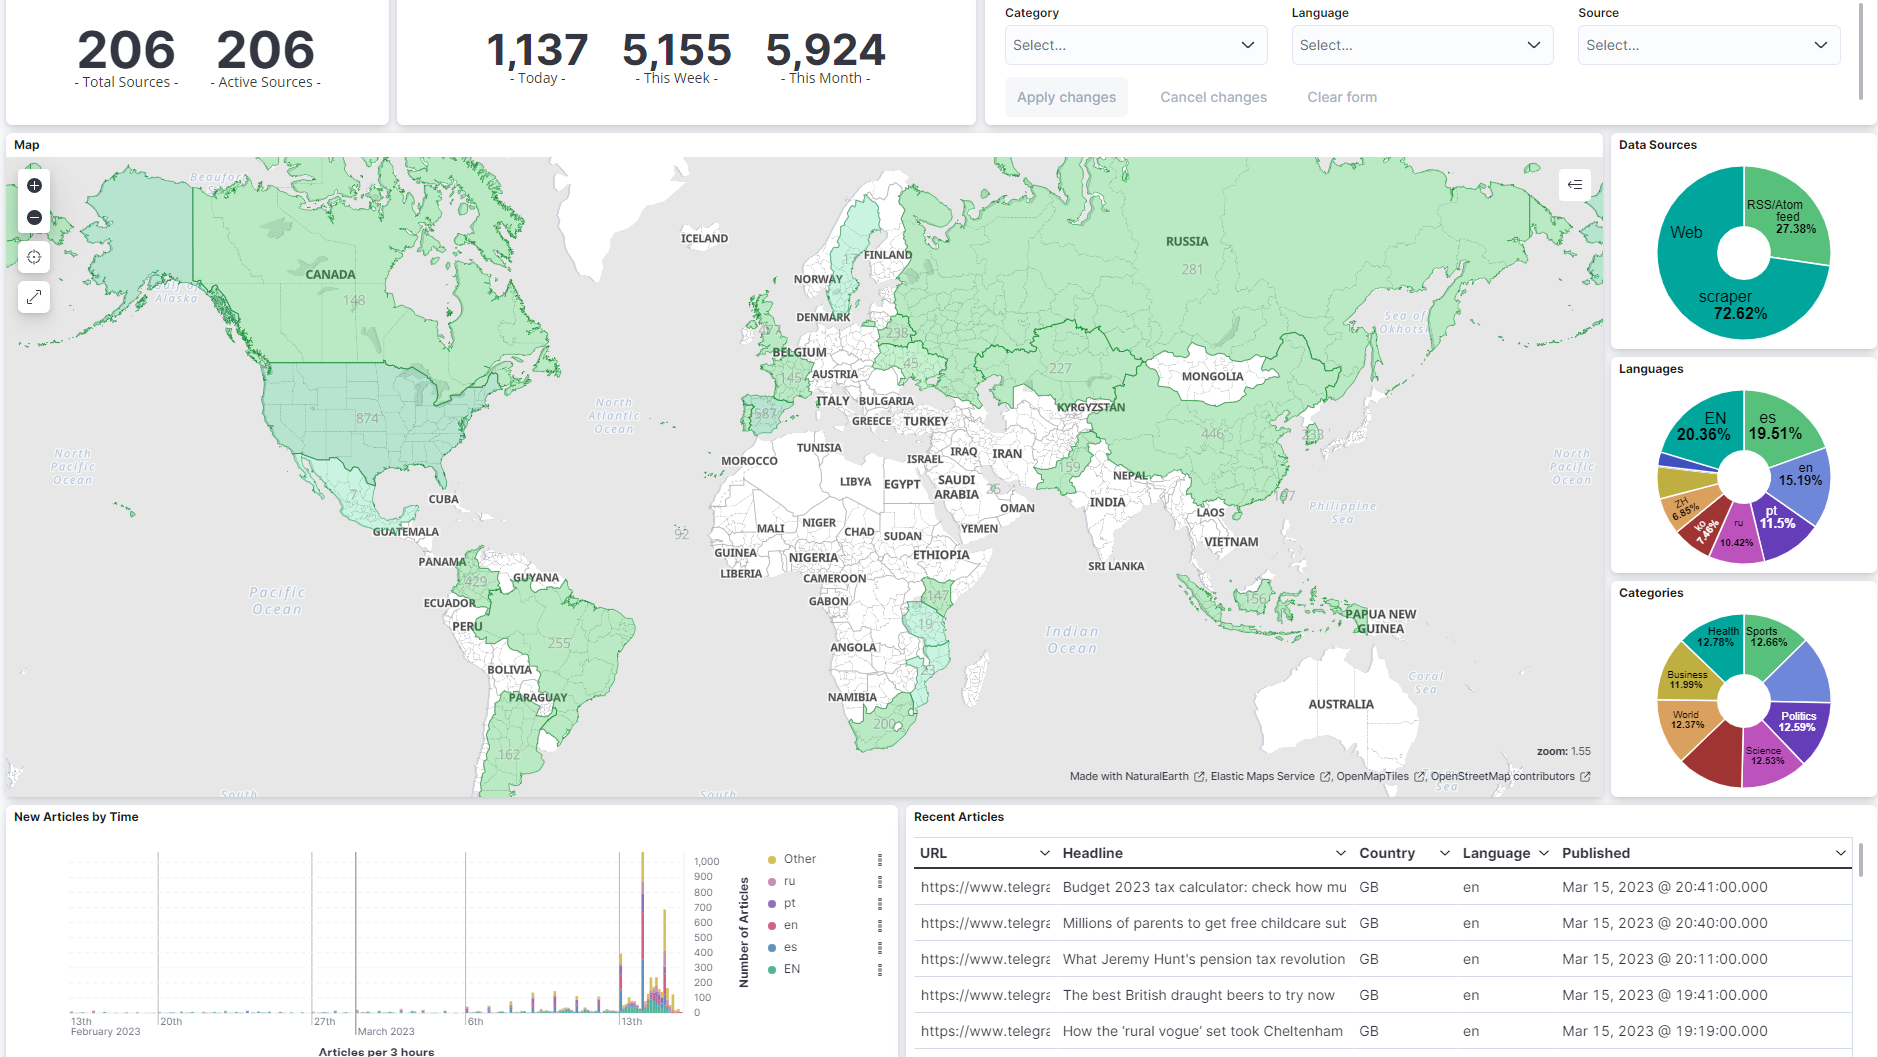
\includegraphics[width=\textwidth]{/Visualisation.png}
\caption{The finished visualisation shown on the web interface}
\label{fig:visualisation}
\end{figure}


\section{Web Interface}
The web interface was implemented with standard HTML, CSS and JavaScript. It is implemented as a single webpage which can show and hide content to give the appearance of two separate pages: management of the system and management of individual sources. This is done to make the website feel more responsive: the pages will switch instantly instead of having to load another webpage. The overall design is inspired by the original BioCaster website, using the same main colours and element styles to create a cohesive visual design with other BioCaster products. The homepage allows for toggling on and off the scraping system, and viewing or hiding the visualisation shown in Figure \ref{fig:visualisation}. The final homepage is shown in Figure \ref{fig:web-interface-homepage}. I chose to let the visualisation be toggled on and off as I found it could be distracting when managing the scraping system.
\begin{figure}[h]
\centering
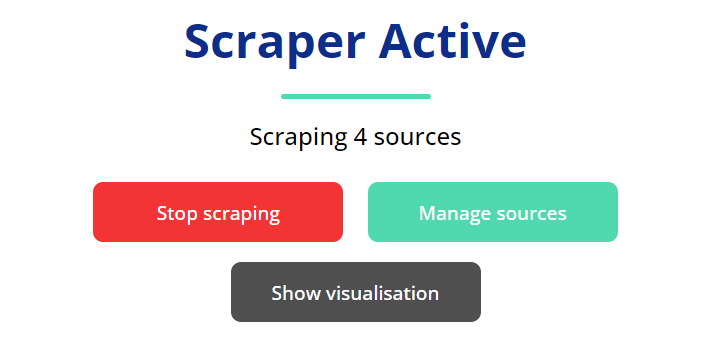
\includegraphics[width=0.5\textwidth]{/web interface homepage.png}
\caption{The homepage of the web interface. White space has been removed for clarity.}
\label{fig:web-interface-homepage}
\end{figure}

The manage sources page shows when sources found their last article, and splits sources which have not found an article in a number of days specified in the config file into a stale section. It also allows for sources to be enabled, disabled, deleted or added. The final manage sources page is shown in Figure \ref{fig:web-interface-manage}. Stale sources are shown at the top of the page, then enabled sources then disabled sources. I chose this order as I believe it represents the order of importance on a management page: Users will be most interested in which sources are stale, and least interested in inactive sources. Stale sources are also highlighted in yellow to add further emphasis and convey a negative sentiment. 

\begin{figure}[!ht]
\centering
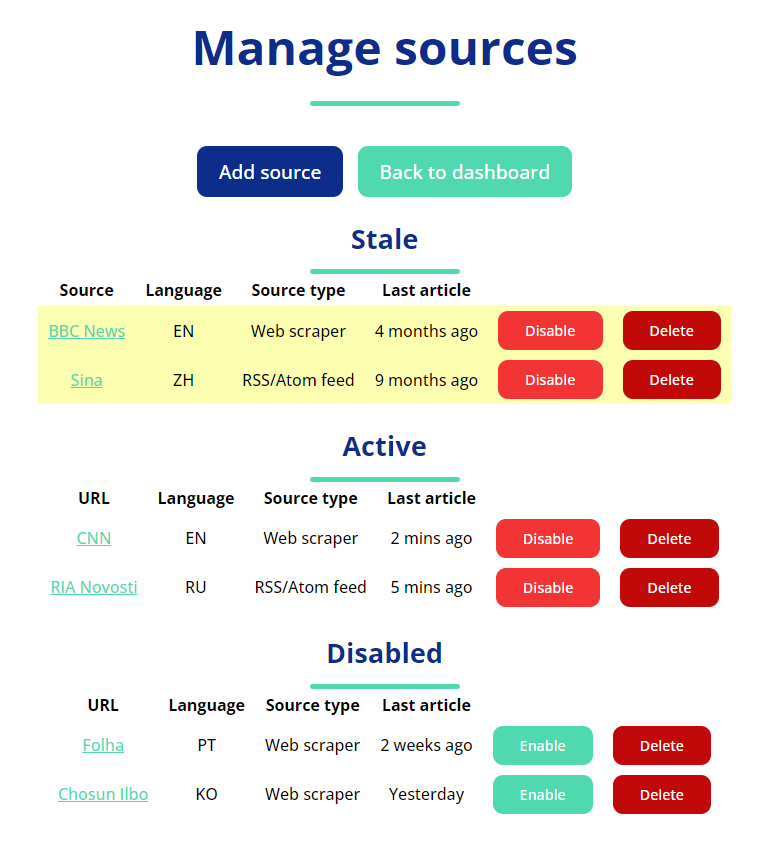
\includegraphics[width=0.75\textwidth]{/web interface manage.png}
\caption{The manage sources page of the web interface. White space has been removed for clarity.}
\label{fig:web-interface-manage}
\end{figure}

\begin{figure}[!ht]
\centering
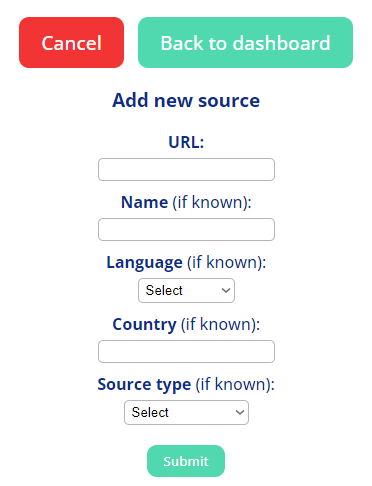
\includegraphics[width=0.33\textwidth]{images/add-source-box.png}
\caption{The add source box displayed when the "Add source" button is clicked on the manage sources page of the web interface.}
\label{fig:add-sources-box}
\end{figure}

The implementation details of the JavaScript responsive elements are contained in the following section, as the logic is connected with requests to and responses from the Python controller.

\section{Web Connector}
The plain HTML/CSS/JavaScript connects to the pythonhttps://github.com/python-eel/Eel code for the scraping system using the python library \emph{eel}\footnote{https://github.com/python-eel/Eel}. This library creates an offline web server using a specified directory and by calling a start method with a specified file, will begin running the web server from the python code.

\subsection{Communication between Python and JavaScript}
By importing "eel.js" in the head section of the index HTML page, an interface is established where the Python and JavaScript modules can pass information aynchronously between each other. Python methods can be exposed to JavaScript using a method decorator, where they can be called in the JavaScript code by calling "eel.<python method name>(<params>)(<callback function>)" where the return values of the python function will be given to the callback function which is called when the values are available. No callback function can be specified to return the value into the function giving the original call (but the value must be awaited as communication is asynchronous). Python modules can also call JavaScript functions but this is not used in this project. The communication between JavaScript and Python is illustrated in figure \ref{fig:eel-communication}

\begin{figure}[!ht]
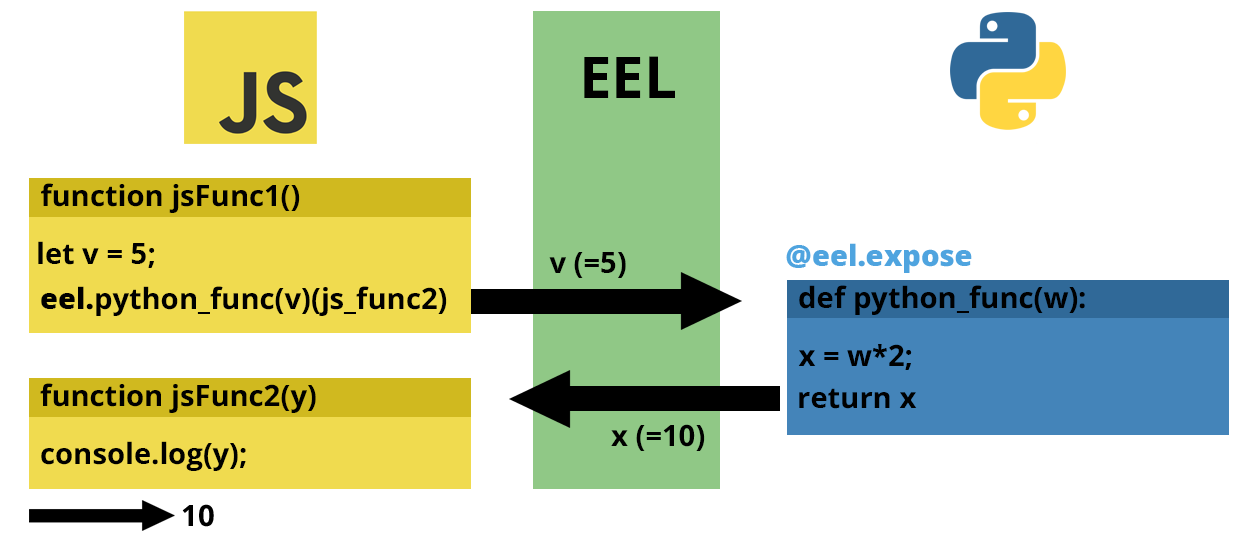
\includegraphics[width=\textwidth]{images/eel-communication.png}
\caption{A diagram showing the process of calling a Python method from the JavaScript code on the web server, using eel. This uses a simple example where jsFunc1 initialises a value, sends the value to python function python\_func which doubles the value and returns it to jsFunc2, which prints the result. The @eel.expose decorator on python\_func makes the function available from the JavaScript file}
\label{fig:eel-communication}
\end{figure}

\subsection{Dynamic Functionality}
The dynamic elements of the page are implemented using JavaScript events: functionality is triggered when the page loads and when buttons are clicked. The visual changes to buttons (e.g. a change in colour of the enable/disable button when toggled) are achieved by adding and removing predefined CSS classes to the clicked elements, and any updates to the state of the system or sources are achieved through communication with the Python controller using eel. An overview of the JavaScript functionality and necessary Python methods for communication is given below:
\subsubsection{Adding sources to the table} \hfill \par
Given a new source, the following steps are performed:
\begin{itemize}
    \item If the source is active, increment the number of active sources.
    \item Get the difference in time between the current time and the time of last new article.
    \item Check if the source is stale (if this difference is larger than the number of days until a source is stale).
    \item Generate a string for the last scrape time (e.g. "5 minutes ago") given this difference.
    \item Decide which table the row should be in (disabled table if it is not active, stale table if it is active and stale, active table otherwise).
    \item Using the date string, stale boolean value and the data from python, build the HTML for a table row.
    \item The ID of the buttons on this new table row will contain the source ID, so that it can be tracked for modifying the source later.    
\end{itemize}
The implementation of this functionality is shown in Appendix \ref{appendix:js-add-sources}.

\subsubsection{JavaScript Events}
\begin{itemize}
    \item \textbf{Page loads: } On page load, the number of days until stale and system state are obtained from the python code, and the state of the Start/stop scraping button is updated accordingly. A method is also started that periodically (once per specified number of seconds) calls the python \textbf{get sources list} method and uses the results to repopulate the tables.
    \item \textbf{Start/stop scraping button:} When clicked, the button calls a method which changes its own text to "Stopping..." or "Starting..." and calls the Python \textbf{toggle scraper} method. When it gets a response, it changes the text and colour of the button (by changing CSS class) to represent the new state and also changes the subtext of the webpage between "Scraping <no. active sources> sources" and "Not currently scraping".
    \item \textbf{Show/hide visualisation button: } When clicked, the button calls a method which changes its own text and sets the display of the visualisation embed to "none" (making it invisible) or "block" (making it appear on the page, below the button).
    \item \textbf{Manage sources button: } When clicked, the button calls a method which toggles the visibility of the div containing the entire manage sources page (changes display from "none" to "block").
    \item \textbf{Back to dashboard button: } When clicked, the button returns the user to the dashboard by setting the display of the div containing the manage sources section to "none".
    \item \textbf{Add source / cancel button: } When clicked, the button changes its own name and colour (from "Add source" in blue to "Cancel" in red) and toggles the visibility of the form for adding sources (shown in Figure \ref{fig:add-sources-box}).
    \item \textbf{Submit button: } When the submit button is clicked, all information is extracted from the form inputs. If the input is valid (contains a name, URL and specifies source type), it is sent to the python \textbf{add source} method. When the source details are returned from this method, the source is added to the active table. If the input is invalid error text is shown.
    \item \textbf{Disable/Enable buttons: } When clicked, the button changes its text to "Disabling..." or "Enabling..." and calls the python \textbf{toggle source} method. When the value is returned, it checks whether the operation was successful. If it was successful, it copies the information from the original table row and deleted the table row. It then creates a new table row in the next table (disabled table if being disabled, otherwise active or stale table depending on the last scrape time of the source). If the operation was unsuccessful, the button text is reverted back to its original value.
    \item \textbf{Delete buttons: } When clicked, the button changes its text to "Deleting..." and calls the python \textbf{delete source} method. When the value is returned, it checks whether the operation was successful. If it was successful, it deletes the table row. If the operation was unsuccessful, the button text is reverted back to "Delete".
\end{itemize}
\hfill \par
\subsubsection{Python Methods}
\begin{itemize}
    \item \textbf{Get days until stale: } Returns the number of days until a source becomes stale
    \item \textbf{Get system state: } Returns a boolean, indicating whether the system is currently active
    \item \textbf{Get sources list: } Returns a list of source crawler objects, including every parameter needed by the JavaScript code (ID, URL, name, language, source type, time of last scrape, if the crawler is active).
    \item \textbf{Toggle system: } Turns the system on or off, returning the new state.
    \item \textbf{Toggle source: } Given a source ID, finds the source in the list of sources and enables/disables it. Returns a boolean indicating whether the action was successful.
    \item \textbf{Delete source: } Given a source ID, finds the source in the list of sources and deletes it (calls the crawler delete method and removes it from the list). Returns a boolean indicating whether the action was successful.
    \item \textbf{Add source: } Given the information from the add source form, creates a new source object and adds it to the source list. Returns the required attributes of the new source object for the JavaScript code (ID, URL, name, language, source type).
\end{itemize}

\section{Controller}
The controller is the module which is run to start the entire system, and when run will perform the following tasks:
\begin{itemize}
    \item Define the web connector python methods
    \item Load variables from the config (whether to auto-disable stale sources, maximum number of sources to scrape, whether to run the web app, days until crawlers are considered stale, minimum number of seconds between scrapes)
    \item Ensures the database indices are created through the database connector
    \item Load the sources from the database and instantiate the crawlers
    \item Instantiate parser(s) and classifier(s)
    \item Build pipelines from data collection to storage in database
    \item If the web app is enabled, start the web app
    \item Start the scraping system
\end{itemize}

\subsection{Multi-threading}
As the eel web server will block the code when running, only continuing to run when the web server is stopped, it is necessary to start the scraping system on a separate thread to allow both to run simultaneously. Some components are required to ensure components are properly synchronised, such as a lock on the list of crawlers, which is passed to parsers and acquired by any part of the code (parser or python web interface function) intending to make changes to the internal state of a scraper, to ensure all operations are performed properly. The scraping system thread also uses an event, which is used to communicate between threads that some condition has been met. In this case, when the web server is stopped it will set the event, and the scraping system periodically checks if the event is set, and will stop if it is. 

\subsection{Pipelines}
The controller defines data pipelines, which control which sources are passed to which parser and classifier, allowing for different sources of data to be processed differently. The pipelines take the form (list of data source types, parser), where the parser is an initialised parser object (with a given classifier). Any sources in the list which are in the list of data source types will be sent to the corresponding parser. To ensure no data duplication, each type of data source can only be sent to one type of parser.

\subsection{Scraping System}
The scraping system is given the list of crawlers and list of pipelines on execution. The algorithm is as follows:
\begin{itemize}
    \item Initialise a list of article URLs for each pipeline
    \item Save the current time as the start time
    \item For each crawler in the list of crawlers
    \begin{itemize}
        \item Block until the scraper system is enabled, checking for the event to be set
        \item Run the crawler to obtain a list of article URLs
        \item Find the first pipeline which includes the type of crawler (or discard the data if there is none)
        \item Add the URLs to the pipelines list
    \end{itemize}
    \item For each pipeline, run the parser on the corresponding list of article URLs
    \item Reset the list of URLs for each pipeline
    \item Get the time elapsed by subtracting the start time from the current time
    \item If the time elapsed is less than the minimum time per scrape, sleep for the rest of the time, checking periodically for the event to be set
    \item Repeat from step 2
\end{itemize}

\section{Summary}
The system is primarily written in python although the web application uses JavaScript. The crawlers use the database connector to update their own state, and concrete implementations use an RSS parser to crawl RSS feeds and a web crawling library to build the profile of a news website and find all article links. The article parser uses the Newspaper3K library to turn the list of URLs into parsed objects, which it sends to the classifier. The BERT classifier is built using Huggingface transformers and uses a previously trained transformer model to categorise each article object from its headline and body, selecting the maximum log likelihood category on inference. The categorised objects are sent by a python database connector to a noSQL elasticsearch database, which directly feeds into the Elastic Kibana visualisation system. These visualisations are embedded on a locally hosted web app by eel, which provides an interface for communication between the web app code and the python code. This interface is used to send the web app updates on the state of sources, and for the web app to send instructions to change source states. The controller orchestrates this process, hosting the web connector functions and building pipelines for data collection and processing.


%==================================================================================================================================


\chapter{News Article Classification Experiment}

\section{Task Definition}
By researching the topics used by the news sources previously collected, as well as considering the topics used in publicly available news classification datasets, a set of six news topic categories was chosen, $C = \{$Entertainment/Arts(0), Sports(1), Politics(2), Science/Technology(3), Business/Finance(4), Health/Welfare(5)$\}$ \par
Given a dataset of news articles $N$ with and corresponding labels $L\in C$, which denotes the category of the given news item. A news article $n \in N$ is composed of sentences, which are composed of words. An arbitrary article $n_i \in N$ can be represented as $(s_1,...,s_I)$, where $I$ denotes the number of sentences in $n_i$. Each sentence $s_j (1 \leq j \leq I)$ can be represented as $(w_1,...,w_J)$, where $J$ denotes the number of words in sentence $s_j$. Each news article will be composed of words in one of six languages: English, French, Spanish, Portuguese, Mandarin or Indonesian. The objective of this experiment is to train a multilingual model M to correctly classify an unseen article $n_new \notin N$ into label $L\in C$. A diagram of the task definition is shown in Figure \ref{fig:task-definition}.

 \begin{figure}[h]
\centering
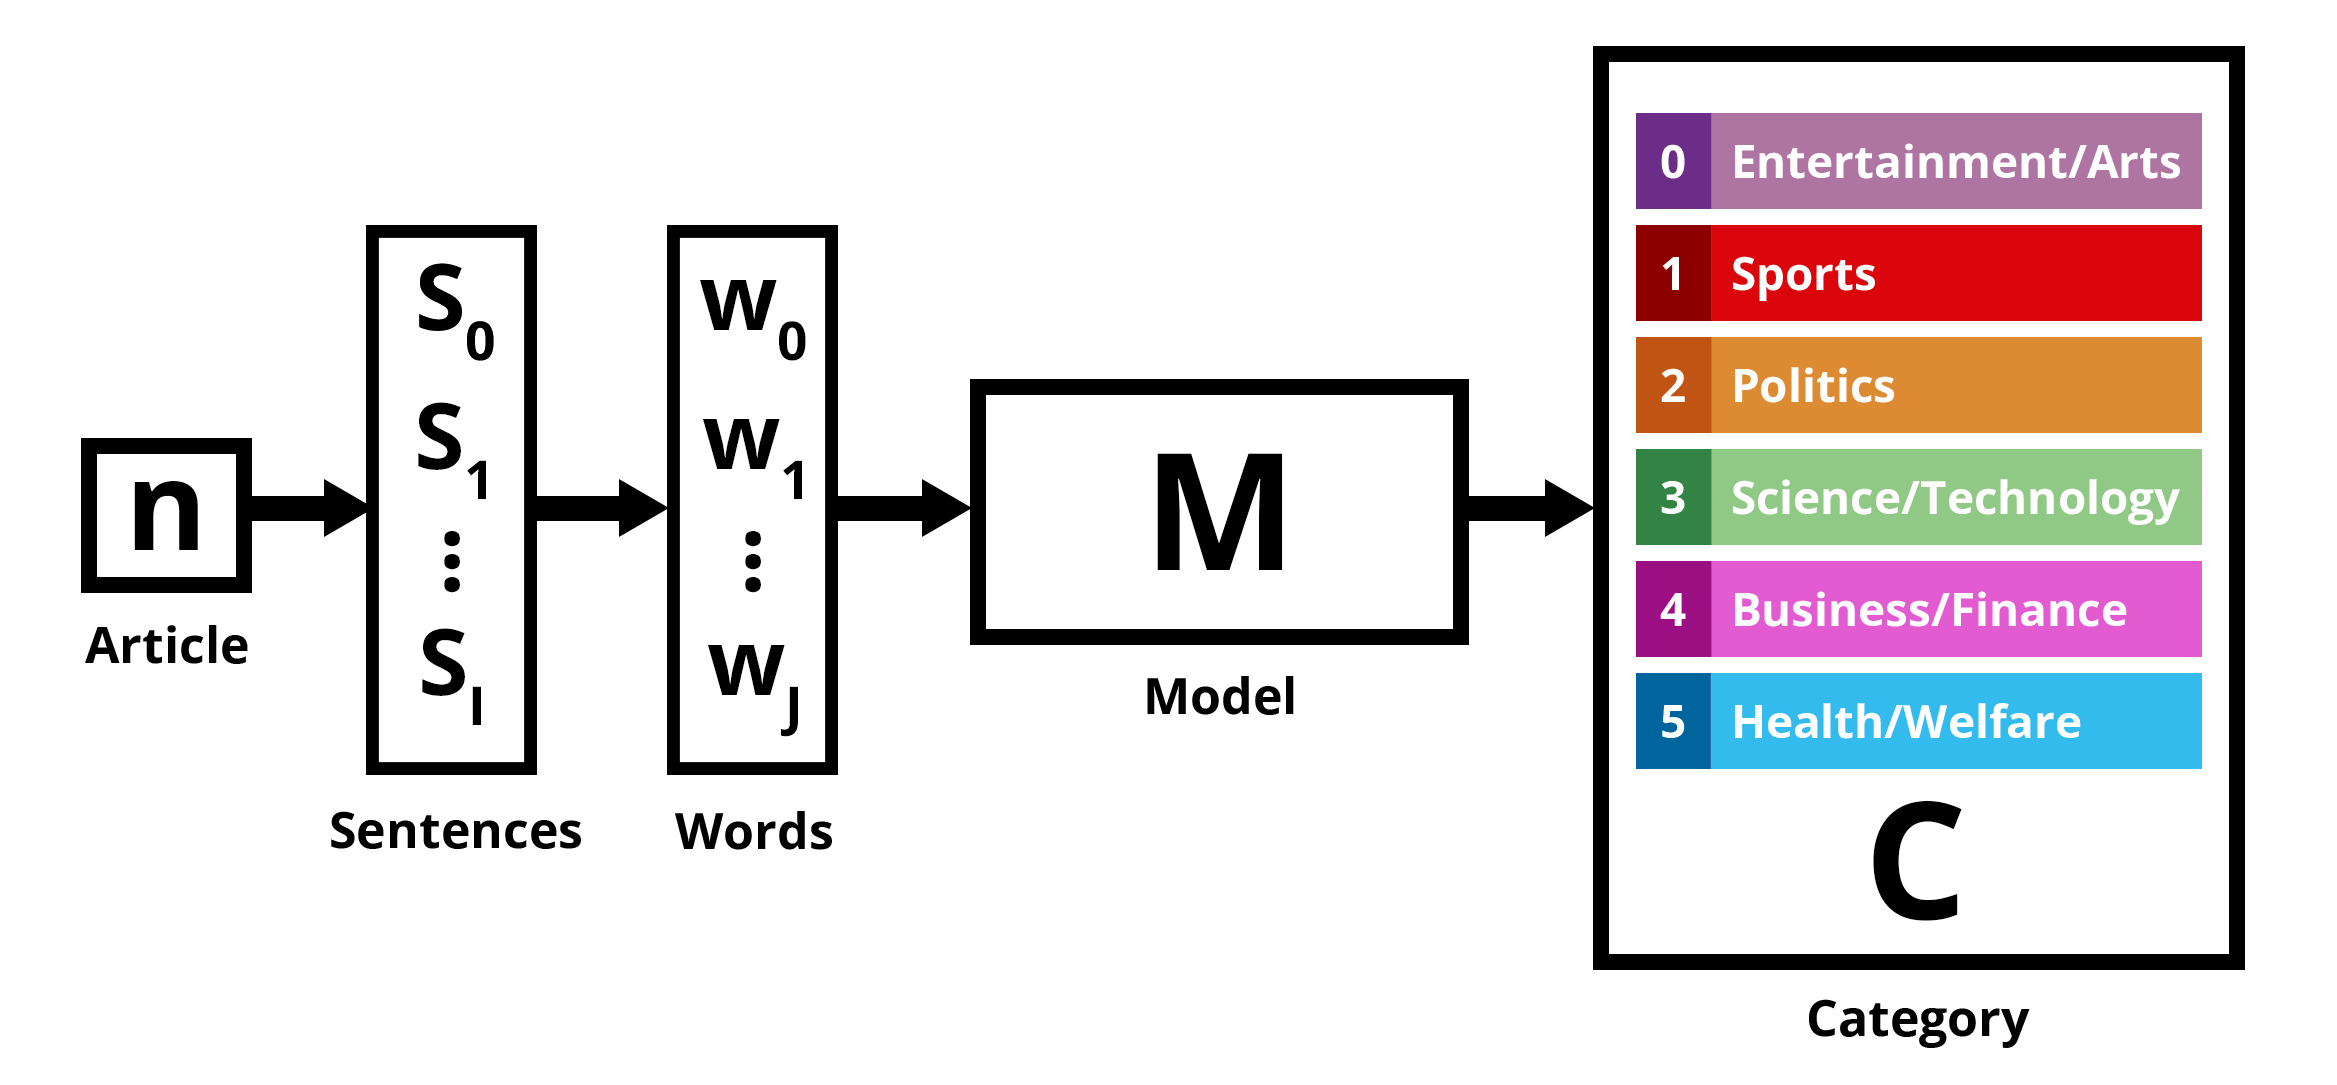
\includegraphics[width=0.8\textwidth]{images/Task Definition.png}
\caption{A diagram representing the flow of a model classifying a news article n, composed of sentences which are composed of words. The news article is eventually assigned a category from C/}
\label{fig:task-definition}
\end{figure}


\section{Multilingual Models}
\subsection{Preliminaries}
\label{section:preliminaries}
\subsubsection{Transformer models} \hfill \par
The first transformer model was introduced in \cite{vaswani2017attention}. It was built by combining an encoder model, which creates a multidimensional vector embedding of input sequences, with a decoder which converts these embeddings to the desired output (e.g. a classification). The architecture is shown in \ref{fig:transformer-architecture}

 \begin{figure}[h]
\centering
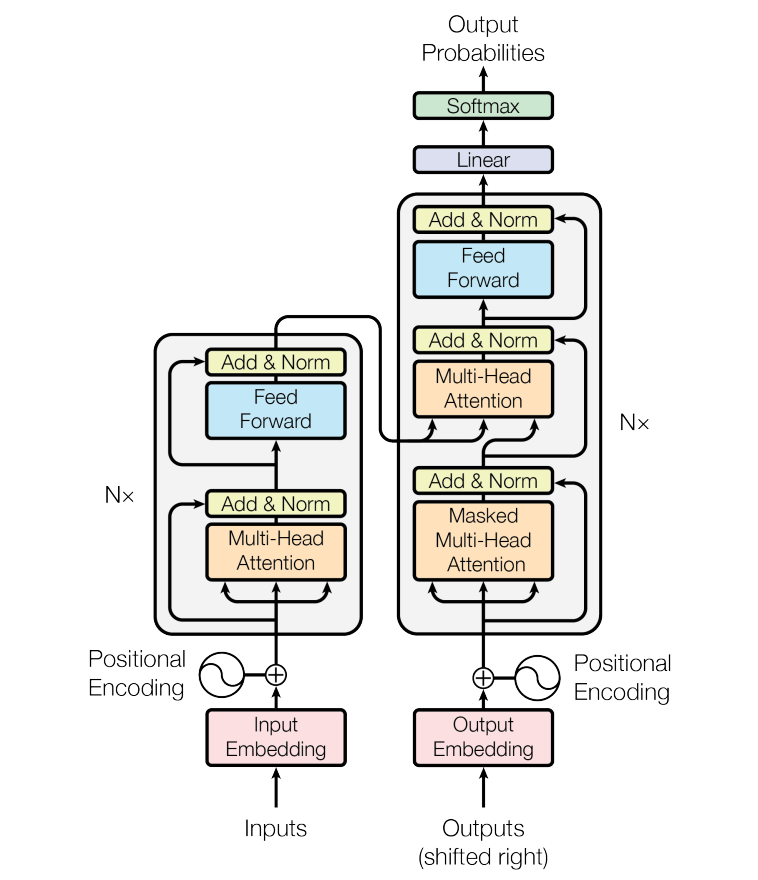
\includegraphics[width=0.6\textwidth]{images/transformer-architecture.png}
\caption{A diagram of the transformer architecture. Obtained from \cite{vaswani2017attention}.}
\label{fig:transformer-architecture}
\end{figure}

Important features of the transformer model which enable its success on text classification tasks include:
\begin{itemize}
    \item Residual connections which allow previous layers output to directly propagate to later layers in the network.
    \item Positional encoding using sine functions to create normalised representation of an items position, instead of using a single index.
    \item Multi-head attention which can represent the importance of other words in the sequence on the current word (explained in later sections)
\end{itemize}

\subsubsection{BERT models and fine-tuning} \hfill \par
A paper by \cite{devlin2018bert} introduced The BERT model (Bidirectional Encoder Representations from Transformers). This model is based on the original transformer architecture, but removes the decoder section in order to become sequence-to-sequence (the model transforms an input sequence to an output sequence). BERT is trained using masked language modelling (MLM), where a percentage of input sentences are hidden from the model and it attempts to guess the missing words. It is also trained on next sentence prediction (NSP) where the model guesses if one sentence follows another. These training tasks allow the model to contextualise words and sentences to create a better understanding and representation of the context of words. When trained on a multilingual corpus, the idea is that these representations are language-agnostic, and allow for successful classification of unseen multilingual data. These representations achieved from pre-training can be fine-tuned to complete a down-stream task, such as multilabel classification, by ignoring all but one of the model outputs and training a classifier on top of this output using a new dataset for the exact downstream task (e.g. news articles with categories) to convert the contextual embeddings of words into a classification label. This process is illustrated in Figure \ref{fig:bert-finetuning}

 \begin{figure}[h]
\centering
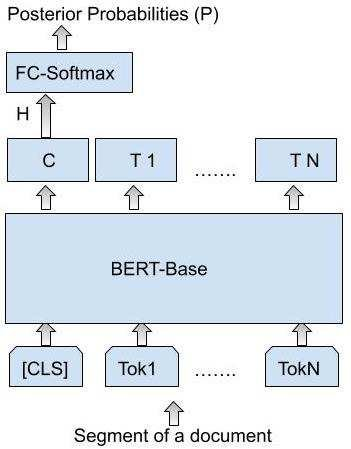
\includegraphics[width=0.4\textwidth]{images/bert finetuning.png}
\caption{A diagram of the architecture of a fine-tuned BERT model on text classification. Obtained from \cite{pappagari2019hierarchical}.}
\label{fig:bert-finetuning}
\end{figure}

\subsubsection{Self-attention} \hfill \par
    BERT models attempt to learn three weight matrices during training, $W_q$, $W_k$ and $W_v$. These are the query, key and value matrices respectively. We can multiply each of the input vectors with these matrices in order to obtain a key, query and value vector for each input. For a given input, we multiply the query vector of the input with the key vector of the other inputs
    to form an attention mask (a representation of how much other words are important to the meaning of this word). This mask is scaled down by the square root of the dimension of the key vector, and a softmax function is performed to normalise values to sum to 1. For each other input, we multiply this weighting by the value vector, and then we sum the result to obtain a weighted combination of the values of other words. This gives the formula, for input query, key and value matrices Q, K, V (which are the concatenation of all input query, key and value vectors):
    $$Attention(Q, K, V) = softmax(\frac{QK^T}{\sqrt{d_k}})V$$
    
\subsubsection{Multi-head attention} \hfill \par
Multi-head attention is an extension of the previous attention mechanism used in models such as BERT. We create multiple attenttion heads which each have different query, key and value weight matrices. We obtain an output matrix for each attention head and concatenate the results. These concatenated results are fed into a fully connected neural network (FCNN) which combines the outputs.

\subsubsection{Fine-tuning the pre-trained models}
These transformer models are very powerful in "understanding" text based on its context, but they are designed to output a text sequence. To allow these models to be used in a classification task, we add a layer on top of the initial BERT model, and only consider one of its outputs (the given class). We train the new model to maximise the number of times this output is correct. This technique allows for training time to be cut down massively in the larger BERT model, as most of the training has been done already and we must only train the model to turn the context embeddings into a classification.


\subsection{Models Used}
\par
The models being used for this experiment are Multilingual BERT (mBERT) and XLM-RoBERTa. The models were trained on many languages, including the six considered here. The key differences between the models are highlighted below:
\subsubsection{Training} \hfill \par
\begin{itemize}
    \item The models are pre-trained on different corpora: mBERT is trained on the Wikipedias of the 104 languages with the most content. XLM-RoBERTa is trained on a larger corpus, using 2.5TB of CommonCrawl data across 100 languages. 
    \item mBERT uses WordPiece tokenization, where each sentence is split into words by spaces or punctuation, and each word is broken into one or more subwords. Each unique subword is associated with a token ID, and input data is converted into a sequence of these token ID's, which are input into the mBERT model for classification. XLM-RoBERTa uses SentencePiece tokenization, a similar subword tokenization scheme which is lossless (it can exactly replicate the input sequence as it retains whitespace and punctuation information) and language independent \citep{kudo2018sentencepiece}. 
\end{itemize}
 

\section{Fine-tuning Scheme}
This experiment uses three datasets: A public English-language news classification dataset \textbf{DS1}, an augmented version of this dataset where all articles have been translated into all 6 languages (including the original English) \textbf{DS2}, and a dataset of real-world news articles collected from our developed scraping system \textbf{DS3}. 
Information on each dataset is detailed in Section \ref{section:datasets}. Data from each dataset was tokenized using the tokenizer associated with the given multilingual model. For each model, the following fine-tuning experiments were performed:
\begin{enumerate}
    \item The models were trained and evaluated on the English public dataset \textbf{DS1}. 
    \item The models were trained and evaluated on the multilingual public dataset \textbf{DS2}.
    \item The previously trained models on \textbf{DS1} were evaluated on the real-world collected data (\textbf{DS3}).
    \item The previously trained models on \textbf{DS2} were evaluated on the real-world collected data (\textbf{DS3}).
    \item The models were trained and evaluated on the real-world collected data (\textbf{DS3}).
\end{enumerate}
A diagram of these experiments is shown in Figure \ref{fig:fintuning-scheme}

\begin{figure}[h]
\centering
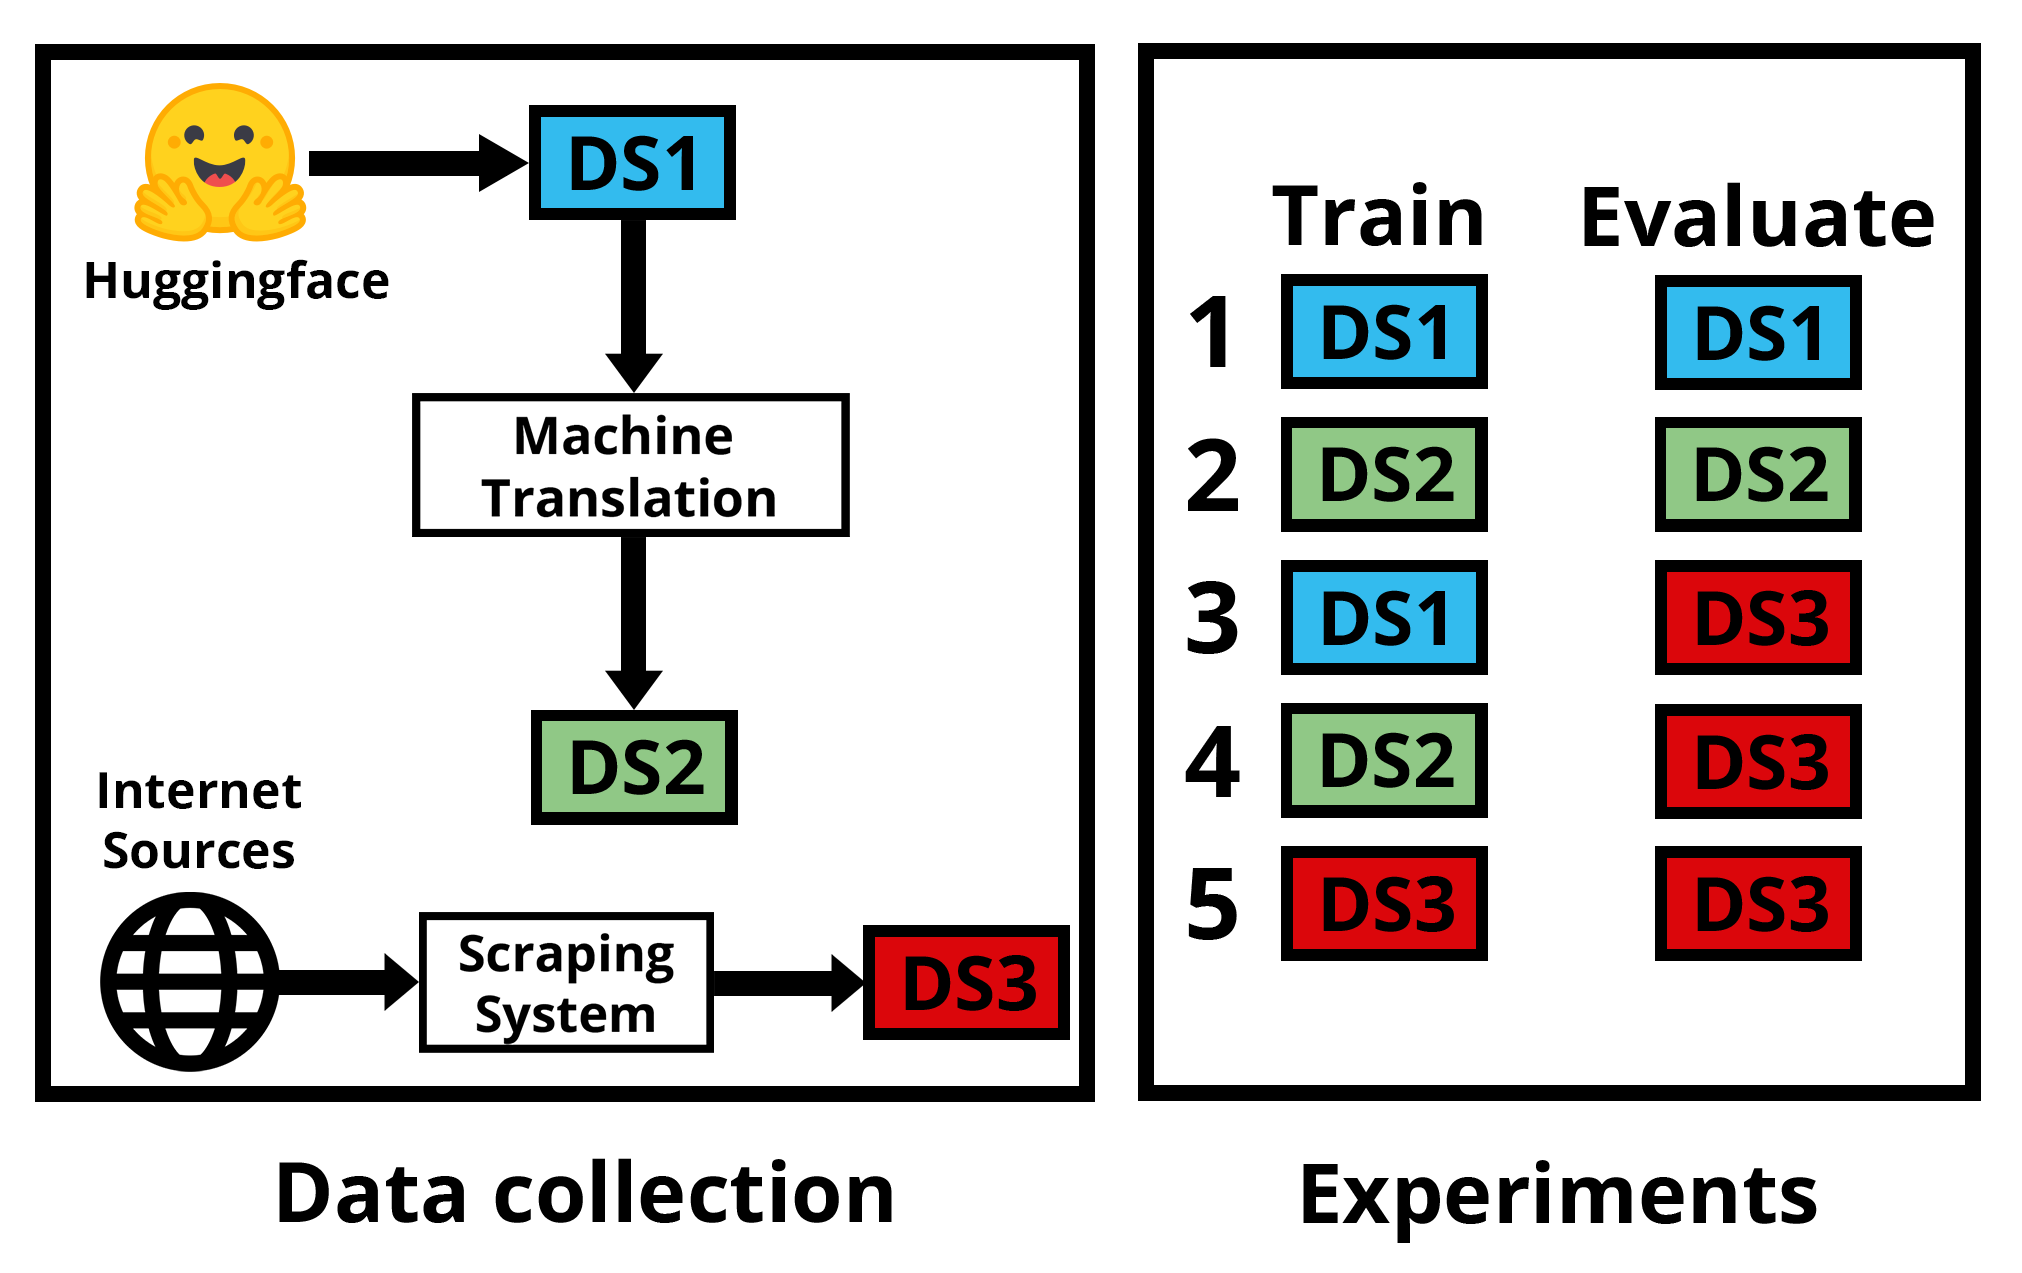
\includegraphics[width=0.6\textwidth]{images/Finetuning Scheme.png}
\caption{A diagram of the finetuning scheme for the news article classification experiment, showing how datasets were obtained and the experiments run for each model (training dataset and evaluation dataset.}
\label{fig:bert-finetuning}
\end{figure}


%==================================================================================================================================
\chapter{Evaluation}

\section{Digital News Surveillance System}
\subsection{Research Overview}
We conducted a usability test on a static version of the web app (not connected to a scraping system) including the final visualisation. We created a questionnaire and sent it to university students and members of the BioCaster research team, receiving 9 responses. This evaluation was conducted following the university ethics guidelines, and a signed ethics checklist is shown in Appendix \ref{appendix:ethics-checklist}. \par
The purpose of the evaluation was to answer the following research questions:
\begin{itemize}
    \item \textbf{RQ1.1: } Does the visualisation provide a complete and effective overview of the data collected?
    \item \textbf{RQ1.2: }Does the interface allow users to easily and effectively manage the underlying web scraping system?
\end{itemize}

The respondents were asked to perform the following tasks, and answer questions on their experiences and opinions on the visualisation and web scraper:
\begin{itemize}
    \item Toggle the scraping system and the visualisation
    \item Adding a source
    \item Enabling/disabling a source
    \item Deleting a source
\end{itemize}

Respondents used a scale from 1-5 (1 being the most negative response) to rate the visualisation on how easy to understand it is and how well it represents the data. They were also asked to rate the web interface on how intuitive, clear to present information and aesthetically appealing it is. Open questions were also asked to elicit more detailed feedback. The results of the rating scale questions are shown in Figure \ref{fig:questionnaire-ratings}

 \begin{figure}[h]
\centering
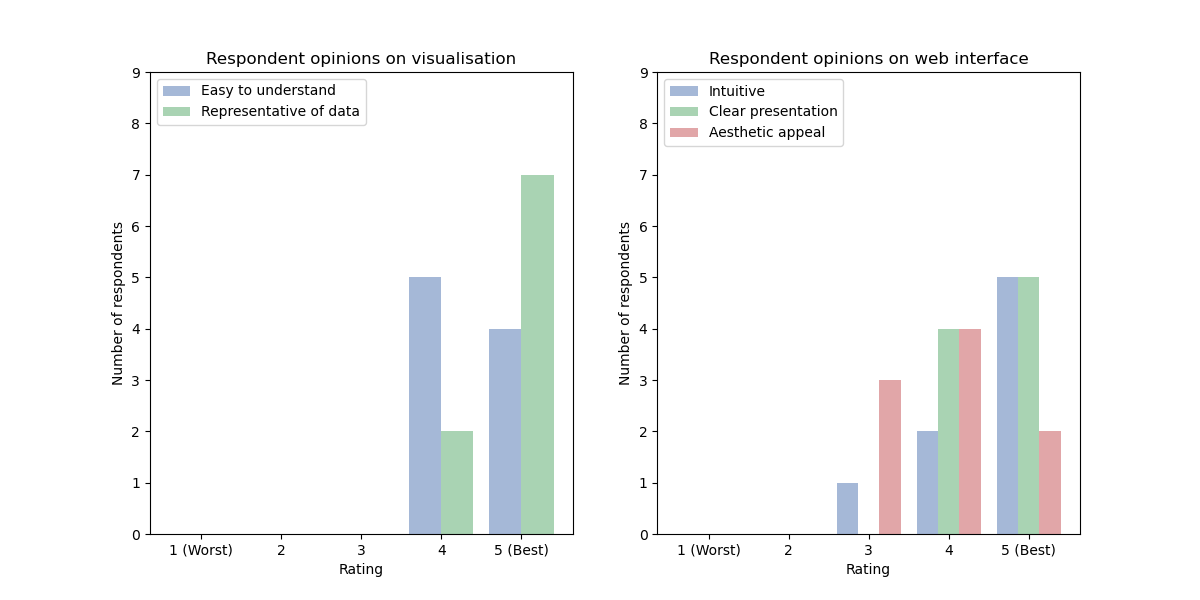
\includegraphics[width=\textwidth]{images/questionnaire_responses.png}
\caption{The results of the rating scale questions of the questionnaire, gauging respondent opinions on various factors of the Kibana visualisation and the web interface.}
\label{fig:questionnaire-ratings}
\end{figure}


The full questionnaire can be found in Appendix \ref{appendix:questionnaire}

\subsection{RQ1.1: Visualisation}
Respondents were asked on a scale from 1-5 (5 being the best response), if they thought the visualisation was easy to understand, and if the visualisation represents the data well. All respondents gave a 4 or higher on both questions, with 4 respondents (44.4\%) rating the visualisation a 5 in ease of understanding and 7 respondents (77.8\%) rating the representation of data collected a 5. These results suggest the visualisation succeeds in representing the data effectively in an easy to understand way, but could use some minor improvements to increase the clarity of data.

Specific examples of feedback given on the visualisation are:
\begin{itemize}
    \item It is unclear what the colours in the density map represent, and the colours are too similar
    \item Filtering recent articles by country when clicking the map would be a useful addition
    \item The visualisation could better fit the whole page without scrolling
    \item Languages should have full names as the two letter representations can be hard to understand
    \item The screen can feel full, it would be useful to be able to adjust components
    \item A pie chart by country isn't effective for geographic distribution, some way to signal proximity would be useful
    \item Top sources by number of articles would be a useful statistic
    \item Categories of article over time may be an interesting metric
    \item More information on source bias/reliability would be useful in considering the reliability of information
    \item The "new articles by time" component can be difficult to interpret
\end{itemize}

The feedback is reasonable, and although many of the recommendations are outside the scope of this project (e.g. source bias and geographic proximity), many of these changes are easy to implement and would immediately improve the visualisation, such as better distinction in the colours and more easily readable language names. The requested additional visualisations could be used to replace less effective visualisations in the current system, such as articles by time.

\subsection{RQ1.2: Web Interface}
Respondents were asked to rate the web interface on how intuitive it is, how clearly information is presented and how aesthetically appealing it is. Results are shown in Figure. Respondents thought the information was clearly presented, with 55.6\% reponding with 5, and the rest with 4, however 12.5\% and 33.3\% of particpants gave the web interface a 3 on intuition and aesthetic appeal respectively, suggesting there is area for improvement on these metrics. 

Specific examples of feedback on the web interface are:
\begin{itemize}
    \item Some filters on the visualisation are hard to remove (requiring a refresh)
    \item Some section fonts are too large
    \item The web app could benefit from an "about" page to describe the purpose
\end{itemize}

Most of the negative feedback come from the problems with the visualisation. The lack of clear purpose shown to some of the respondents may have worsened the experience but this will not be an issue in the final product, as the web app is only intended to be used by internal team members.

\subsection{Conclusions}
From the results, the visualisation and web interface seems to at least moderately succeed in all of its goals. There were some suggestions for extra features or visualisation components and criticism of existing components, but overall the respondents believed the visualisation was a complete representation of the data. The visualisations are mostly clear and effective, but particularly the colour of the map could use some clarity, both in displaying its purpose and in more visual distinction between different levels of density. The full names of languages should also be added to make the data more clear to people viewing it. \par
Despite the limitations of the usability test, the web interface shows promise as an effective method of managing the underlying scraping system. Feedback was less positive overall than with the visualisation, but the opinion seems to be tied to technical issues with the visualisation and the lack of clarity in the experiment and mock interface itself, rather than as a product of interface design (which had only a few minor complaints and some compliments).

\subsection{Limitations}
Due to the nature of the web interface (hosted on a local web server), it was difficult to host an online version of the site which would be connected to a real scraping system. This meant that it was only possible to evaluate on a mock interface, which some respondents mentioned made the web interface less intuitive as they cannot directly see the results of their actions on the system. In addition, due to many of the respondents working in different countries and having busy schedules, it was impossible to conduct a live evaluation where respondents could be monitored using the app. This would have been more useful to understand the exact feedback given and directly view any bugs or technical issues. The low sample size (n=9) of the evaluation also reduces the ability to generalise findings on the effectiveness of the web interface and visualisation, and limits the range of feedback available.



\section{Multilingual News Article Classification}

\subsection{Research Questions}
In many languages, particularly minority languages, little to no labelled public datasets are available for topic classification of news, meaning models cannot be trained by traditional means. This creates difficulty when trying to perform real-time classification tasks on news written in minority languages, for purposes such as creating disease alerts. We will investigate the efficacy of some techniques and approaches for multilingual document classification, by investigating the following research questions: 
\begin{itemize}
\item \textbf{RQ2.1: }How effective is machine translation of English articles into other languages, as a method of upsampling, in increasing the effectiveness of multilingual models? 
\item \textbf{RQ2.2: }How effective are models trained on public data (both in English and translated into all 6 languages) when used to classify collected news data directly from sources across the six languages? 
\item \textbf{RQ2.3: }What level of performance can be achieved by multilingual models when trained and evaluated on collected articles from sources in each of the six languages?
\end{itemize}

\subsection{Datasets}
\label{section:datasets}
\subsubsection{Public data} \hfill \par
The dataset used is a dataset made available on huggingface by \cite{valurankdata}. The data originally consists of 3,722 classified English-language news articles scraped from various online news sources with 7 topic labels: World, Politics, Tech, Entertainment, Sport, Business, Health, and Science. To match the categories being considered in this experiment, articles belonging to the "World" category were dropped, and those belonging to the "Tech" and "Science" categories were merged into a new "Science/Technology" category. An augmented dataset was also created by adding copies of each article translated into each of the other five languages (French, Spanish, Portuguese, Mandarin and Indonesian). Translations were obtained using the Google translate API through the python library \emph{googletrans}\footnote{https://pypi.org/project/googletrans/}. The distribution of topics in the original and augmented datasets is shown in Table \ref{table:valurankstats} and Figure \ref{fig:public_cat_dist}.

\begin{table}[h]
\begin{tabular}{llllllll}
\hline
\multicolumn{1}{c}{\textbf{}} & \multicolumn{7}{c}{\textbf{Number of Documents}}                                                                                          \\ \hline
                              & \textbf{Entertainment} & \textbf{Sports} & \textbf{Politics} & \textbf{Science/}   & \textbf{Business} & \textbf{Health} & \textbf{Total} \\
                              & \textbf{}              &                 &                   & \textbf{Technology} & \textbf{}         & \textbf{}       &                \\ \hline
\textbf{Original}             & 485                    & 454             & 442               & 838                 & 461               & 467             & \textbf{3147}  \\
\textbf{Translated}           & 2910                   & 2724            & 2652              & 5028                & 2766              & 2802            & \textbf{18882} \\ \hline
\end{tabular}
\caption{Category distribution of the Valurank news categorization dataset. This table includes the original dataset and the augmented version obtained from adding the translations of each article in each of the other 5 languages.}
\label{table:valurankstats}
\end{table}


\begin{figure}[h]
\centering
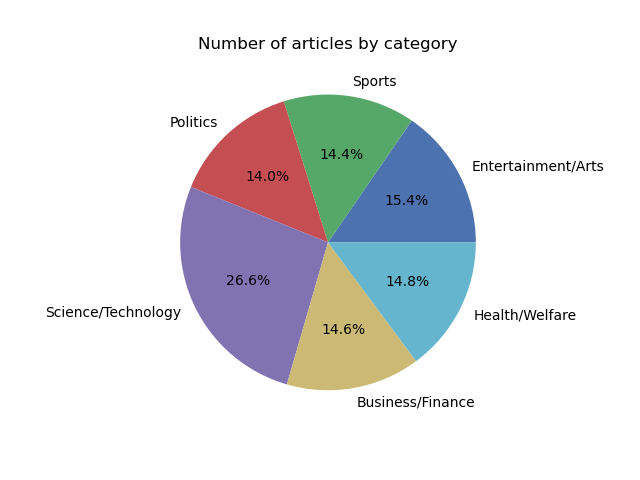
\includegraphics[width=0.8\textwidth]{images/public-cats.png}
\caption{The distribution of categories in the public Valurank dataset}
\label{fig:public_cat_dist}
\end{figure}

\subsubsection{Real-world data collection} \hfill \par
We collected news articles from some of the most popular online news sources across the six languages. The list of six topics used was created after considering the most common category sections in news sources across different languages, and combining similar categories which were often combined by the original sources (such as business and finance). A set of keywords relevant to each category was also generated, shown in Figure \ref{fig:dataset_category_keywords}. Each collected article was self-labelled by the source, and the articles were collected and categorised using the previously developed scraping system, with each article URL obtained and classified either through topic-specific RSS feeds or by matching the URL of article webpages with topics which match category keywords (e.g. abcnews.go.com/Sports). A complete list of data sources used is available in the appendix (link specific appendix). \par

\begin{table}[h]
\begin{tabular}{ll}
\hline
\textbf{Category}           & \textbf{Keywords}                                                 \\ \hline
\textbf{Entertainment/Arts} & Entertainment, Art, Arts, Culture, Movies, Cinema, Music,         \\
\textbf{}                   & Books, Theater, Television, Dance, Celebrity                      \\
\textbf{Sports}             & Sport, Sports, Soccer, Football, Basketball, Tennis, Golf, Rugby, \\
\textbf{}                   & Motorsport, Formula 1, Physical Education                         \\
\textbf{Politics}           & Politics, Election, Parliament                                    \\
\textbf{Science/Technology} & Science, Technology, Tech, SciTech, Space, Physics                \\
\textbf{Business/Finance}   & Business, Finance, Economy, Stock exchange, Stock market, Market, \\
\textbf{}                   & Money, Investment                                                 \\
\textbf{Health/Welfare}     & Health, Welfare, Coronavirus, Pharma, Pharmacy                    \\ \hline
\end{tabular}
\caption{List of category keywords used for collecting news data. Sources which had RSS feeds or specific URL patterns with these keywords were selected for the corresponding category.}
\label{fig:dataset_category_keywords}
\end{table}

Each collected article URL was parsed using the \emph{Newspaper3k}\footnote{https://newspaper.readthedocs.io/en/latest/} library. Any article with a main body under 100 characters in length was discarded, and the article headline and body were concatenated into one text field, used for classification. Originally data was collected for 10 different languages, but only the six considered returned a sufficient number of results for model training. In the final dataset, "Business/Finance" and "Science/Technology" articles in Mandarin were downsampled in order to balance the categories, by randomly dropping articles of these categories and languages at probabilities of $p=0.75$ and $p=0.5$ respectively. \par
The distribution of articles by category and language is shown below in Table \ref{table:collectedstats} and in Figure \ref{fig:collected-distributions}.

\begin{table}[h]
\begin{tabular}{llllllll}
\hline
\textbf{Language}   & \multicolumn{6}{c}{\textbf{Category}}                                                                                       &                 \\ \hline
\textbf{}           & \textbf{Entertainment/} & \textbf{Sports} & \textbf{Politics} & \textbf{Science/}     & \textbf{Business/} & \textbf{Health/}   & \textbf{Total}  \\
\textbf{}           & \textbf{Arts}         & \textbf{}       & \textbf{}         & \textbf{Technology} & \textbf{Finance} & \textbf{Welfare} & \textbf{}       \\ \hline
\textbf{Mandarin}   & 511                    & 706             & 329               & 961                  & 802               & 217               & 3,526           \\
\textbf{English}    & 885                    & 682             & 435               & 607                  & 493               & 390               & 3,492           \\
\textbf{Indonesian} & 478                    & 545             & 71                & 295                  & 598               & 255               & 2,242           \\
\textbf{French}     & 342                    & 369             & 138               & 88                   & 235               & 114               & 1,286           \\
\textbf{Portuguese} & 136                    & 197             & 196               & 240                  & 232               & 167               & 1,168           \\
\textbf{Spanish}    & 203                    & 400             & 159               & 48                   & 238               & 84                & 1,132           \\ \hline
\textbf{Total}      & 2,555                  & 2,899           & 1,328             & 2,239                & 2,598             & 1,227             & \textbf{12,846}
\\ \hline
\end{tabular}
\caption{The distribution of collected news articles by language and category.}
\label{table:collectedstats}
\end{table}

\begin{figure}[h]
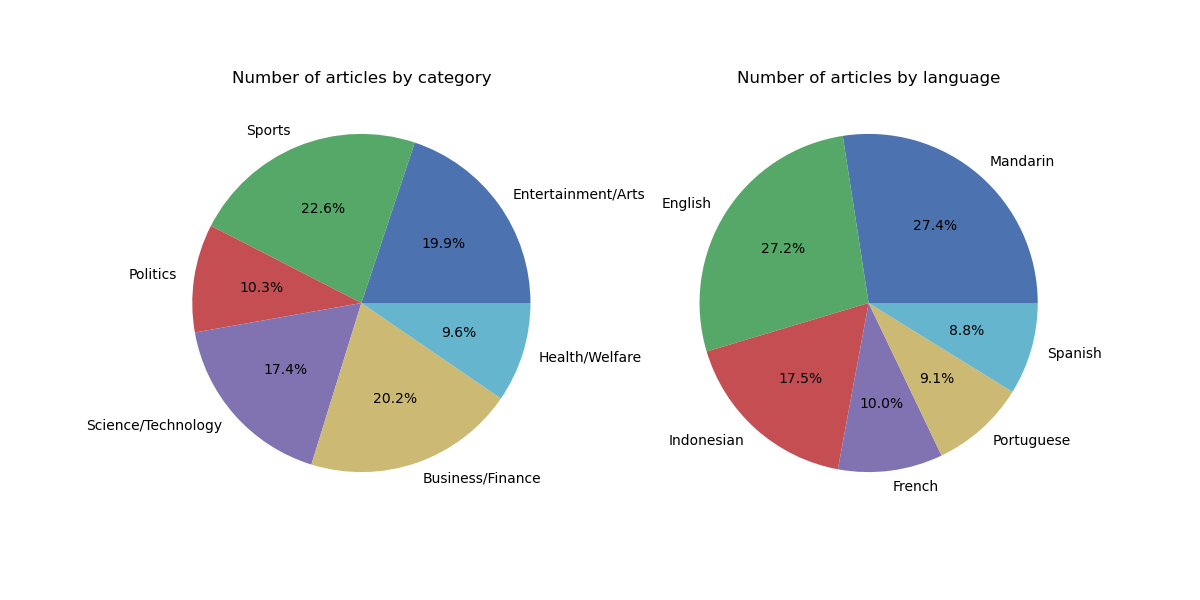
\includegraphics[width=\textwidth]{images/real_data_distributions.png}
\caption{The distribution of categories and languages in the public Valurank dataset}
\label{fig:collected-distributions}
\end{figure}

\subsection{Evaluation Setting}
\subsubsection{Baselines} \hfill \par
To test the effectiveness of machine translation upsampling, we will use the models trained on the English only public dataset as a benchmark, to measure how much (if any) accuracy increases using translation to augment the dataset. When comparing how models trained on public data transfer to collected real-world multilingual data, we can use static models which do not learn from the data as a baseline. In this case, we use two static baseline models: a model which uses stratified sampling (it samples a prediction for an input randomly, using the category densities as a probability distribution) and most common sampling (always predicts the category with the most training examples). This allows us to consider how much of what the model learns from the public data can be applied to the real-world data.

\subsubsection{Hyperparameters} \hfill \par
The hyperparameters investigated in this experiment were batch size (how many examples are used in training per backpropagation cycle), number of epochs (how many times does the model repeat the training data) and learning rate (how quickly does the model update its parameters to improve predictions). The values considered are based on the recommendations and experiments from the original BERT paper, by \cite{devlin2018bert}, and shown in Table \ref{table:hparams}. In each case, an exhaustive grid search was performed (24 trials) on the hyperparameter values and the highest accuracy model was chosen for the evaluation. The optimal hyperparameters found for each model is shown in Appendix \ref{appendix:optimal-hparams}

\begin{table}[h]
\begin{tabular}{ll}
\hline
\textbf{Parameter}  & \textbf{Values}        \\ \hline
\textbf{Batch size} & 16, 32                \\
Number of epochs    & 2, 3, 4                \\
Learning rate       & \SI{5e-5}, \SI{4e-5}, \SI{3e-5}, \SI{2e-5}. \\ \hline
\end{tabular}
\caption{A list of hyperparameters tuned before training each model for classification. In each case, a grid search was performed with these values.}
\label{table:hparams}
\end{table}

\subsubsection{Data splitting} \hfill \par
Because the categories in our datasets were not too imbalanced (the largest category disparity is around 2:1) we decided that data can be split randomly into a train and a test split. For each dataset, a train/test split of 80/20 (80\% training data) was used.

\subsubsection{Evaluation metrics}
We will evaluate each model's performance using the  classification accuracy (which percentage of predicted categories are correct), as well as its weighted F1 score. These ratings are widely used in machine learning literature, including classification tasks \citep{alam2020bangla, al2020multiple, ranasinghe2020multilingual}. F1 score is a common metric for effectiveness in classification problems, which aims to balance precision and recall. In binary (two label) classification, precision measures the proportion of predicted positive labels (true positives and false positives) are true positives. Recall measures how many of the true positive data items (true positive and false negative predictions) were classified correctly as positive (true positive). F1 score is the harmonic mean of precision and recall, and aims to balance these metrics to favour a model which avoids false positives but also misses as few positive examples. \par
In a multiclass context, the F1 score for each possible label is calculated separately and combined. There are different methods for combining these scores, including taking a global average (micro-F1) or taking an unweighted sum of per-category averages (macro-F!). In this experiment we will use weighted F1 score, which takes a weighted average of category F1 scores based on the category weighting (the proportion of the data represented by this category). The weighted F1 score for a dataset $D$ with categories $\{c_1, c_2, ..., c_N\}$ can be calculated as:
$$Precision=\frac{TP}{TP+FP}$$ 
$$Recall=\frac{TP}{TP+FN}
$$ $$F1 \ score=2 \cdot \frac{Precision \cdot Recall}{Precision + Recall}$$
$$Weighted \ F1=\sum_{i=1}^{N}w_i \cdot F1 \ score_i \quad \quad \quad \quad w_i=\frac{|D_{d \in c_i}|}{|D|}$$

Where TP, FP and FN are the number of true positive, false positive and false negative classifications. Each experiment will be repeated for three training runs, and the mean and standard deviation of the accuracy and weighted F1 scores will be used as metrics for the effectiveness of each model.

\subsection{RQ2.1: Effectiveness of Translation Upsampling}
Shown in Table \ref{table:backtranslation-effectiveness} are the results of training and testing the multilingual models in the original English-only and augmented translated Valurank public dataset. The results show that all models achieve very high ($>95\%$) accuracy and F1 score for the public dataset. We can also see that both models achieve an increased performance of 2-3\% on the larger translated dataset, reaching near-perfect ($>98\%$) accuracy and F1 score in both cases. In both cases, the mBERT model performs slightly better than the XLM-RoBERTa model, but there is very little difference ($<1\%$) in accuracy. This suggests that upsampling can be an effective method of improving classification accuracy by providing more samples.

\begin{table}[h]
\begin{tabular}{lllll}
\hline
\textbf{Model}   & \multicolumn{2}{l}{\textbf{English Data}} & \multicolumn{2}{l}{\textbf{Multilingual Data}} \\ \cline{2-5} 
                 & \textbf{Accuracy}    & \textbf{Weighted F1}   & \textbf{Accuracy}   & \textbf{Weighted F1}   \\ \hline 
\textbf{mBERT-base}       & \textbf{96.50$\pm$0.22}    & \textbf{96.52$\pm$0.22}          & \textbf{98.77$\pm$0.10}       & \textbf{98.77$\pm$0.10}          \\
\textbf{XLM-RoBERTa-base} & 95.66$\pm$0.37    & 95.66$\pm$0.34          & 98.70$\pm$0.00       & 98.70$\pm$0.00   
     \\ \hline
\end{tabular}
\caption{Accuracy and weighted F1 score (mean $\pm$ standard deviation) of models trained and tested on the Valurank public dataset, both in English only and translated into 5 additional languages, over 3 training runs. The most effective model for each dataset is denoted in \textbf{bold.}}
\label{table:backtranslation-effectiveness}
\end{table}

\subsection{RQ2.2: Transfer of Models to Real-world Data}  \hfill \par

Table \ref{table:transferability} shows the results of transferring the models trained on public data to real-world collected data. The trained multilingual models perform significantly better than the baseline models, but achieve significantly lower accuracies and F1 scores than when they are evaluated on the public datasets. This suggests there are some similarities between public news datasets and real-world news, but not enough that public datasets can be an effective substitute. The XLM-RoBERTa model seems to generalise more effectively on both training sets, achieving 7-9\% better accuracy and F1 score than the corresponding mBERT model. In both models, there is no significant difference in how the models perform on real-world collected data when trained on English or multilingual data.

\begin{table}[h]
\begin{tabular}{lllll}
\hline
\textbf{Model}               & \textbf{English Data} &             & \textbf{Multilingual Data} &             \\ \cline{2-5} 
                             & Accuracy              & Weighted F1 & Accuracy                   & Weighted F1 \\ \hline
\textbf{Stratified Sampling} & 17.72\%$\pm$0.80     & 17.74$\pm$0.80 & 17.72\%$\pm$0.80     & 17.74$\pm$0.80            \\
\textbf{Most Common}         & 23.54\%$\pm$0.00     & 8.97$\pm$0.00 & 23.54\%$\pm$0.00     & 8.97$\pm$0.00 \\ \hline
\textbf{mBERT-base}          & 65.78\%$\pm$0.21     & 65.96$\pm$0.14         & 66.03\%$\pm$0.51        & 66.00$\pm$0.48         \\
\textbf{XLM-RoBERTa-base}    & \textbf{74.78\%$\pm$1.27}  & \textbf{74.92$\pm$1.24}        & \textbf{73.38\%$\pm$0.00}   & \textbf{73.34$\pm$0.00}        \\ \hline
\end{tabular}
\caption{Accuracy and weighted F1 score (mean $\pm$ standard deviation) of stratified sampling and most common static baseline models, as well as multilingual models trained on the Valurank public dataset (English only and translated into 5 additional languages). All models were evaluated on the collected multilingual dataset, over 3 training runs. The most effective model for each dataset is denoted in \textbf{bold.}}
\label{table:transferability}
\end{table}

\subsection{RQ2.3: Classifying Real-world Data}

Table \ref{table:realworld-effectiveness} shows the results of training and testing the multilingual models on the real-world collected dataset. There is little significant difference between the two multilingual models, with XLM-RoBERTa achieving slightly higher accuracy and F1 scores of ~89.5\%. Both models achieve a lower accuracy on the collected dataset than on either of the public datasets, but perform significantly better when trained on the same dataset than on the public dataset. This suggests that real-world news may be more difficult to accurately classify. \par
Table \ref{table:confusion_matrix} shows the confusion matrix for the best performing model (XLM-RoBERTA-base) on the real-world test data. We can see that the most common misclassifications are predicting Business/Finance as Science/Technology (55 occurrences), predicting Politics as Business/Finance (48 occurrences) and predicting Science/Technology as Business/Finance (39 occurrences). This suggests that there may be large similarities or overlap between these three categories.

\begin{table}[h]
\begin{tabular}{lll}
\hline
\textbf{Model}   & \textbf{Accuracy} & \textbf{Weighted F1} \\ \hline
\textbf{mBERT-base}       & 87.81\%$\pm$0.24     & 87.75$\pm$0.26        \\
\textbf{XLM-RoBERTa-base} & \textbf{89.40\%$\pm$0.15}     & \textbf{89.34$\pm$0.17}                 \\ \hline
\end{tabular}
\caption{Accuracy and weighted F1 score (mean $\pm$ standard deviation) of models trained and tested on the collected multilingual dataset, over 3 training runs. The most effective model for each dataset is denoted in \textbf{bold.}}
\label{table:realworld-effectiveness}
\end{table}

\begin{table}[h]
\begin{tabular}{lllllll}
\hline
\multicolumn{1}{c}{\textbf{Actual label}} & \multicolumn{6}{c}{\textbf{Predicted label}}                                                                                                                                                                                            \\ \hline
                                          & \textbf{Entertainment/}              & \textbf{Sports}                      & \textbf{Politics}                    & \textbf{Science/}                    & \textbf{Business/}                   & \textbf{Health/}                     \\
                                          & \textbf{Arts}                        & \textbf{}                            & \textbf{}                            & \textbf{Technology}                  & \textbf{Finance}                     & \textbf{Welfare}                     \\ \hline
\textbf{Entertainment/Arts}               & \cellcolor[HTML]{67FD9A}\textbf{445} & \cellcolor[HTML]{FFCCC9}6            & \cellcolor[HTML]{FFCCC9}1            & \cellcolor[HTML]{FD6864}19           & \cellcolor[HTML]{FFCCC9}4            & \cellcolor[HTML]{FFCCC9}6            \\
\textbf{Sports}                           & \cellcolor[HTML]{FFCCC9}6            & \cellcolor[HTML]{67FD9A}\textbf{558} & 0                                    & \cellcolor[HTML]{FFCCC9}3            & \cellcolor[HTML]{FFCCC9}2             & 0                                    \\
\textbf{Politics}                         & \cellcolor[HTML]{FFCCC9}5            & \cellcolor[HTML]{FFCCC9}1            & \cellcolor[HTML]{67FD9A}\textbf{196} & \cellcolor[HTML]{FD6864}11           & \cellcolor[HTML]{FE0000}48           & \cellcolor[HTML]{FD6864}15           \\
\textbf{Science/Technology}               & \cellcolor[HTML]{FFCCC9}4            & \cellcolor[HTML]{FFCCC9}3            & 0                                    & \cellcolor[HTML]{67FD9A}\textbf{385} & \cellcolor[HTML]{FE0000}39           & \cellcolor[HTML]{FFCCC9}8            \\
\textbf{Business/Finance}                 & \cellcolor[HTML]{FFCCC9}6            & \cellcolor[HTML]{FFCCC9}3            & \cellcolor[HTML]{FFCCC9}8            & \cellcolor[HTML]{FE0000}55           & \cellcolor[HTML]{67FD9A}\textbf{486} & \cellcolor[HTML]{FFCCC9}8            \\
\textbf{Health/Welfare}                   & \cellcolor[HTML]{FFCCC9}3            & \cellcolor[HTML]{FFCCC9}2            & 0                                    & \cellcolor[HTML]{FD6864}14           & \cellcolor[HTML]{FD6864}14           & \cellcolor[HTML]{67FD9A}\textbf{211} \\ \hline
\end{tabular}
\caption{Confusion matrix for the XLM-RoBERTa-base on real-world multilingual test data. The matrix shows where the prediction errors lay, and is colour coded so that deeper reds indicate more common misclassifications (the green diagonal shows correct classifications)}
\label{table:confusion_matrix}
\end{table}

\subsection{Conclusions}
\textbf{RQ2.1: } Machine translation of news articles shows some promise as a means of upsampling annotated public data, yielding an improvement in classification accuracy and F1 score over training on the monolingual dataset (as shown in Table \ref{table:backtranslation-effectiveness}. For smaller datasets, this could be an effective way of synthesising much more training data to allow multilingual models to learn more effectively and achieve increased performance. Future research is required to determine if machine translation is as effective on multilingual data. \par
\textbf{RQ2.2: } The large increase in performance from the baseline models when the multilingual models are trained on public data and evaluated on collected data (as shown in Table \ref{table:transferability}) suggests that the multilingual models have learned some patterns which still apply to real-world data. The decrease in accuracy and F1 score when generalising to real-world data is likely due to the differences in how news articles are categorised and written across languages. Even when translated into multiple other languages, the public dataset only captures the writing and categorisation conventions of English-language news and these may not generalise effectively between language and source type. As an example, some Chinese sources categorise lottery results as "Sports", whereas English-language sources almost never do this. This suggests that for effective classification of news in minority languages, effort should be taken to obtain training data which is written in the language instead of relying on machine translation. \par
\textbf{RQ2.3: } While performance on real-world datasets (shown in Table \ref{table:realworld-effectiveness}) remains high (~89\% accuracy) there is a significant decrease in performance in the models from the public dataset evaluation (shown in table \ref{table:backtranslation-effectiveness}. This is likely because real-world data is less simple to sort into one category than most publicly annotated data: category boundaries are often not clear and even human annotators may disagree on classifications, many articles could be considered to fit into multiple categories and some are even given multiple categories by the original news source. The model performs very well on Sports articles, where there is less overlap with other categories and hence less ambiguity, but often confuses Business/Finance, Politics and Science/Technology articles. In real-world articles, these subject areas often overlap: many political decisions affect the economy, and technology is often a topic of political debate. Future research could consider a more appropriate task for news article classification, such as multiclass classification with more labels, using human-annotated data.

\subsection{Limitations}
Due to the lack of public labelled data for news article topic classification in many languages, in order to consider this task in a multilingual setting it was necessary to collect my own public data using RSS feeds and web scraping. The data collected is not annotated or reviewed by a human, and instead solely relies on the tagging of the news sources being used. This means that training data may be mislabelled or contain errors, and results achieved through experiments using these data may not be as valid as results obtained from manually annotated data. \par


%==================================================================================================================================


\chapter{Conclusion}    
\section{Project Summary}
In this project, we considered an existing digital disease surveillance system, BioCaster, and attempted to improve the areas in which it was lacking. In particular, we designed a robust news collection system which can retrieve information from a wide variety of sources at a higher level of detail than the current BioCaster system. We developed a system which is easily extensible and configurable and allows for many different types of data source to be collected and used in disease alerts, and implemented 2 of these methods: RSS feeds and news website scraping. We implemented a system for extracting details from these news articles and a classifier system to assign each article a topic. In addition, we reworked the original BioCaster visualisations to reflect the new data collected and created a web interface where this visualisation can be viewed, and the web scraping system can be controlled. Data from the usability test suggests that this visualisation represents the data well and the web interface is mostly intuitive and clearly presents the information to the user. \par

We also obtained results from experimentation with multilingual news classification which suggests machine translation upsampling is plausible to increase the accuracy of multilingual models, and trained a model which can achieve ~90\% accuracy on real-world collected news. 

\section{Future Work}
\subsection{Web Scraping System}
While being designed to easily accommodate the adding of new sources, there are many potentially useful sources of information which this project doesn't implement, which could be implemented by future projects. These include google news data, social media data and search trends. \par
The system has some room to improve in efficiency. For example, a future system may use multi-threading to parse multiple articles at once, removing the bottleneck of communication with the internet in the current single-threaded system. 
\subsection{Multilingual News Article Classification}
Research by \cite{wu2020all} suggests that multilingual BERT is less effective in transferring its results to low-resource languages, and pre-training on a multilingual task instead of masked language modelling (MLM) would produce a better model for language transfer. Due to limited resources and time, this pre-training was not possible in this evaluation, but a future study could consider how these methods are applied to the task of multilingual news classification. To impeove the validity of results, future research could collect human-labelled news category datasets for use in training the multilingual models, instead of assuming the validity of articles scraped from the internet and labelled by the data source.











%==================================================================================================================================
%  APPENDICES  
\begin{appendices}
\chapter{List of data sources for real-world dataset}
\label{appendix:data-sources}
\begin{obeylines}
\textbf{Entertainment/Arts:}
EN:
http://feeds.bbci.co.uk/news/entertainment\_and\_arts/rss.xml
https://rss.nytimes.com/services/xml/rss/nyt/Arts.xml
https://rss.nytimes.com/services/xml/rss/nyt/Books.xml
https://rss.nytimes.com/services/xml/rss/nyt/Movies.xml
https://rss.nytimes.com/services/xml/rss/nyt/Music.xml
https://rss.nytimes.com/services/xml/rss/nyt/Television.xml
https://rss.nytimes.com/services/xml/rss/nyt/Theater.xml
https://rss.nytimes.com/services/xml/rss/nyt/Dance.xml
http://rss.cnn.com/rss/edition\_entertainment.rss
https://www.theguardian.com/uk/film/rss
https://www.theguardian.com/uk/tv-and-radio/rss
https://www.theguardian.com/books/rss
https://www.theguardian.com/artanddesign/rss
https://www.theguardian.com/stage/rss
https://rss.cbc.ca/lineup/arts.xml
https://globalnews.ca/entertainment/feed/
https://abcnews.go.com/Entertainment
https://www.stuff.co.nz/entertainment
https://www.jamaicaobserver.com/rssfeed/entertainment/
https://www.thenews.com.pk/rss/1/10
https://www.rte.ie/entertainment/
FR:
https://www.lefigaro.fr/rss/figaro\_cinema.xml
https://www.lefigaro.fr/rss/figaro\_musique.xml
https://www.lefigaro.fr/rss/figaro\_livres.xml
https://www.lefigaro.fr/rss/figaro\_theatre.xml
https://www.lefigaro.fr/rss/figaro\_arts-expositions.xml
https://www.lemonde.fr/en/cinema/rss\_full.xml
https://www.lemonde.fr/en/music/rss\_full.xml
https://www.lemonde.fr/en/television-radio/rss\_full.xml
https://www.lemonde.fr/en/books/rss\_full.xml
https://www.lemonde.fr/en/arts/rss\_full.xml
https://www.liberation.fr/cinema/
https://www.liberation.fr/arts/
https://www.liberation.fr/musique/
https://www.liberation.fr/livres/
https://www.lexpress.fr/theatre/
https://www.lexpress.fr/musique/
https://www.lexpress.fr/livre/
https://www.lexpress.fr/art/
https://www.lexpress.fr/cinema/
https://www.lapresse.ca/arts/rss
https://www.ledevoir.com/rss/section/culture.xml?id=48
https://lapresse.tn/category/culture/feed/
https://www.europe1.fr/rss/culture.xml
ES:
https://e00-elmundo.uecdn.es/elmundo/rss/television.xml
http://www.abc.es/rss/feeds/abc\_Cultura.xml
http://www.abc.es/rss/feeds/abc\_Libros.xml
http://www.abc.es/rss/feeds/abc\_Teatro.xml
http://www.abc.es/rss/feeds/abc\_Arte.xml
https://elpais.com/cultura/
https://elpais.com/television/
https://www.lanacion.com.ar/cultura/
https://www.elnacional.com/entretenimiento/
https://pulsoslp.com.mx/cultura
https://www.jornada.com.mx/rss/cultura.xml
https://www.eltiempo.com/rss/cultura.xml
https://www.elespectador.com/entretenimiento/
PT:
https://www.publico.pt/culturaipsilon
https://www.dn.pt/cultura/
http://g1.globo.com/dynamo/pop-arte/rss2.xml
http://g1.globo.com/dynamo/musica/rss2.xml
https://www.cartacapital.com.br/cultura/
https://expressodasilhas.cv/cultura
ID:
https://www.jawapos.com/entertainment/
https://www.pikiran-rakyat.com/entertainment
https://www.suara.com/rss/entertainment
https://www.tribunnews.com/seleb
https://www.suara.com/entertainment
ZH:
https://ent.sina.com.cn/
https://ent.huanqiu.com/
https://art.huanqiu.com/
https://news.mingpao.com/rss/pns/s00016.xml
https://ent.ltn.com.tw/
https://www.zaobao.com.sg/entertainment/

\textbf{Sports:}
EN:
http://newsrss.bbc.co.uk/rss/sportonline\_uk\_edition/front\_page/rss.xml
http://newsrss.bbc.co.uk/rss/sportonline\_uk\_edition/football/rss.xml
http://newsrss.bbc.co.uk/rss/sportonline\_uk\_edition/cricket/rss.xml
http://newsrss.bbc.co.uk/rss/sportonline\_uk\_edition/rugby\_union/rss.xml
http://newsrss.bbc.co.uk/rss/sportonline\_uk\_edition/rugby\_league/rss.xml
http://newsrss.bbc.co.uk/rss/sportonline\_uk\_edition/golf/rss.xml
http://newsrss.bbc.co.uk/rss/sportonline\_uk\_edition/boxing/rss.xml
http://newsrss.bbc.co.uk/rss/sportonline\_uk\_edition/athletics/rss.xml
https://rss.nytimes.com/services/xml/rss/nyt/Sports.xml
http://rss.cnn.com/rss/edition\_sport.rss
http://rss.cnn.com/rss/edition\_football.rss
http://rss.cnn.com/rss/edition\_motorsport.rss
http://rss.cnn.com/rss/edition\_tennis.rss
http://rss.cnn.com/rss/edition\_golf.rss
https://www.theguardian.com/uk/sport/rss
https://rss.cbc.ca/lineup/sports.xml
https://globalnews.ca/sports/feed/
https://abcnews.go.com/Sports
https://www.stuff.co.nz/sport
https://www.jamaicaobserver.com/rssfeed/sport/
https://www.thenews.com.pk/rss/1/3
https://www.rte.ie/sport/
FR:
https://www.lefigaro.fr/rss/figaro\_football.xml
https://www.lefigaro.fr/rss/figaro\_football-transfert.xml
https://www.lefigaro.fr/rss/figaro\_rugby.xml
https://www.lefigaro.fr/rss/figaro\_tennis.xml
https://www.lefigaro.fr/rss/figaro\_formule-1.xml
https://www.lefigaro.fr/rss/figaro\_basket.xml
https://www.lemonde.fr/en/sports/rss\_full.xml
https://www.lemonde.fr/en/football//rss\_full.xml
https://www.lemonde.fr/en/rugby/rss\_full.xml
https://www.lemonde.fr/en/basket/rss\_full.xml
https://www.liberation.fr/sports/
https://www.lapresse.ca/sports/rss
https://www.ledevoir.com/rss/section/sports.xml?id=85
https://lapresse.tn/category/sport/feed/
https://www.europe1.fr/rss/sport.xml
ES:
https://e00-elmundo.uecdn.es/elmundodeporte/rss/portada.xml
https://e00-elmundo.uecdn.es/elmundodeporte/rss/futbol.xml
https://e00-elmundo.uecdn.es/elmundodeporte/rss/baloncesto.xml
https://e00-elmundo.uecdn.es/elmundodeporte/rss/ciclismo.xml
https://e00-elmundo.uecdn.es/elmundodeporte/rss/golf.xml
https://e00-elmundo.uecdn.es/elmundodeporte/rss/tenis.xml
http://www.abc.es/rss/feeds/abc\_Deportes.xml
http://www.abc.es/rss/feeds/abc\_Futbol.xml
http://www.abc.es/rss/feeds/abc\_Baloncesto.xml
http://www.abc.es/rss/feeds/abc\_Tenis.xml
http://www.abc.es/rss/feeds/abc\_Automovilismo.xml
https://elpais.com/deportes/
https://www.lanacion.com.ar/deportes/
https://www.elnacional.com/deportes/
https://pulsoslp.com.mx/meta
https://www.jornada.com.mx/rss/deportes.xml
https://www.eltiempo.com/rss/deportes.xml
https://www.elespectador.com/deportes/
PT:
https://www.publico.pt/desporto
https://www.dn.pt/desporto/
http://feeds.jn.pt/JN-Desporto
https://feeds.folha.uol.com.br/esporte/rss091.xml
https://expressodasilhas.cv/desporto
ID:
https://bola.kompas.com/
https://sport.republika.co.id/
https://www.jawapos.com/sports/
https://www.jawapos.com/sepak-bola-indonesia/
https://www.pikiran-rakyat.com/olahraga/
https://www.pikiran-rakyat.com/bola/
https://www.suara.com/rss/bola
https://www.tribunnews.com/sport
https://sport.detik.com/
https://www.suara.com/sport
ZH:
https://sports.sina.com.cn/
https://sports.huanqiu.com/
https://news.mingpao.com/rss/pns/s00015.xml
https://sports.ltn.com.tw/
https://www.zaobao.com.sg/sports
http://www.people.com.cn/rss/sports.xml

\textbf{Politics:}
EN:
http://feeds.bbci.co.uk/news/politics/rss.xml
https://rss.nytimes.com/services/xml/rss/nyt/Politics.xml
https://www.statnews.com/category/politics/feed/
https://www.theguardian.com/politics/rss
https://globalnews.ca/politics/feed/
https://abcnews.go.com/Politics
http://www.scoop.co.nz/storyindex/index.rss?s.c=PO
https://www.stuff.co.nz/politics
https://rss.cbc.ca/lineup/politics.xml
https://www.thenews.com.pk/rss/1/8
FR:
https://www.lefigaro.fr/rss/figaro\_politique\_le-scan.xml
https://www.liberation.fr/politique/
https://www.lexpress.fr/politique/
https://www.lapresse.ca/actualites/politique/rss
https://www.ledevoir.com/rss/section/politique.xml?id=51
https://www.europe1.fr/rss/politique.xml
ES:
https://www.lanacion.com.ar/politica/
https://www.jornada.com.mx/rss/politica.xml
https://www.eltiempo.com/rss/politica.xml
https://www.elespectador.com/politica/
PT:
https://www.publico.pt/politica/
https://www.dn.pt/politica/
https://feeds.folha.uol.com.br/poder/rss091.xml
http://g1.globo.com/dynamo/politica/mensalao/rss2.xml
https://www.cartacapital.com.br/politica
https://expressodasilhas.cv/politica
https://jornalnoticias.co.mz/politica/
ID:
https://www.jawapos.com/politik/
https://www.tribunnews.com/mata-lokal-memilih
https://news.detik.com/pemilu
https://sorotpolitik.kompas.com/
https://kilasparlemen.kompas.com/
ZH:
https://news.ltn.com.tw/politics/
http://www.people.com.cn/rss/politics.xml
http://cpc.people.com.cn/
https://politics.gmw.cn/

\textbf{Science/Technology:}
EN:
http://feeds.bbci.co.uk/news/technology/rss.xml
https://rss.nytimes.com/services/xml/rss/nyt/Technology.xml
https://rss.nytimes.com/services/xml/rss/nyt/PersonalTech.xml
http://rss.cnn.com/rss/edition\_technology.rss
https://www.theguardian.com/uk/technology/rss
https://rss.cbc.ca/lineup/technology.xml
https://globalnews.ca/tech/feed/
https://abcnews.go.com/Technology
https://www.thenews.com.pk/rss/1/11
http://www.scoop.co.nz/storyindex/index.rss?s.c=SC
https://www.newscientist.com/subject/technology/feed/
https://www.newscientist.com/subject/physics/feed/
https://www.newscientist.com/subject/space/feed/
FR:
https://www.lefigaro.fr/rss/figaro\_secteur\_high-tech.xml
https://www.lapresse.ca/affaires/techno/rss
https://www.ledevoir.com/rss/section/societe/science.xml
https://www.europe1.fr/rss/technologies.xml
https://www.europe1.fr/rss/sciences.xml
ES:
https://e00-elmundo.uecdn.es/elmundo/rss/ciencia.xml
http://www.abc.es/rss/feeds/abc\_Ciencia.xml
http://www.abc.es/rss/feeds/abc\_Tecnologia.xml
https://elpais.com/ciencia/
https://elpais.com/tecnologia/
https://www.lanacion.com.ar/tecnologia/
https://www.lanacion.com.ar/ciencia/
https://www.elnacional.com/ciencia-tecnologia/
https://pulsoslp.com.mx/cienciaytecnologia
https://www.jornada.com.mx/rss/ciencias.xml
https://www.eltiempo.com/rss/tecnosfera.xml
https://www.elespectador.com/tecnologia/
https://www.elespectador.com/ciencia/
PT:
https://www.publico.pt/tecnologia
https://www.dn.pt/ciencia/
https://feeds.folha.uol.com.br/tec/rss091.xml
https://feeds.folha.uol.com.br/ciencia/rss091.xml
http://g1.globo.com/dynamo/tecnologia/rss2.xml
https://www.cartacapital.com.br/tecnologia
ID:
https://tekno.kompas.com/
https://www.kompas.com/sains
https://tekno.republika.co.id/
https://www.suara.com/rss/tekno
https://zetizen.jawapos.com/rss/science
https://zetizen.jawapos.com/rss/techno
https://www.pikiran-rakyat.com/teknologi/
https://www.tribunnews.com/techno
https://www.suara.com/tekno
ZH:
https://tech.sina.com.cn/
https://tech.huanqiu.com/
AR:
https://www.aljazeera.net/tech/
https://www.aljazeera.net/science/
https://alwafd.news/%D8%AA%D9%83%D9%86%D9%88%D9%84%D9%88%D8%AC%D9%8A%D8%A7
https://www.albayan.ae/technology
https://www.eremnews.com/sciences-technology

\textbf{Business/Finance:}
EN:
http://feeds.bbci.co.uk/news/business/rss.xml
https://rss.nytimes.com/services/xml/rss/nyt/Business.xml
https://rss.nytimes.com/services/xml/rss/nyt/SmallBusiness.xml
https://rss.nytimes.com/services/xml/rss/nyt/Economy.xml
http://rss.cnn.com/rss/money\_news\_international.rss
https://www.theguardian.com/uk/business/rss
https://www.theguardian.com/uk/money/rss
https://rss.cbc.ca/lineup/business.xml
https://globalnews.ca/money/feed/
https://abcnews.go.com/Business
http://www.scoop.co.nz/storyindex/index.rss?s.c=BU
https://www.stuff.co.nz/business
https://www.jamaicaobserver.com/rssfeed/business/
https://www.thenews.com.pk/rss/2/15
https://www.rte.ie/business/
FR:
https://www.lefigaro.fr/rss/figaro\_societes.xml
https://www.lefigaro.fr/rss/figaro\_bourse.xml
https://www.lemonde.fr/en/economy/rss\_full.xml
https://www.lemonde.fr/en/money-investments/rss\_full.xml
https://www.liberation.fr/economie/
https://www.lapresse.ca/affaires/economie/rss
https://www.lapresse.ca/affaires/marches/rss
https://www.lapresse.ca/affaires/entreprises/rss
https://www.ledevoir.com/rss/section/economie.xml?id=49
https://lapresse.tn/category/economie/feed/
https://www.europe1.fr/rss/economie.xml
ES:
https://e00-elmundo.uecdn.es/elmundo/rss/economia.xml
http://www.abc.es/rss/feeds/abc\_Economia.xml
https://elpais.com/economia/
https://www.lanacion.com.ar/economia/
https://www.elnacional.com/economia/
https://www.jornada.com.mx/rss/economia.xml
https://www.eltiempo.com/rss/economia.xml
https://www.elespectador.com/economia/
PT:
https://www.publico.pt/economia
https://www.dn.pt/dinheiro/
http://feeds.jn.pt/JN-Economia
https://feeds.folha.uol.com.br/mercado/rss091.xml
http://g1.globo.com/dynamo/economia/rss2.xml
https://www.cartacapital.com.br/economia
https://expressodasilhas.cv/economia
https://jornalnoticias.co.mz/economia/
https://jornalnoticias.co.mz/desporto/
ID:
https://money.kompas.com/
https://ekonomi.republika.co.id/
https://www.jawapos.com/ekonomi/
https://www.pikiran-rakyat.com/ekonomi/
https://www.suara.com/rss/bisnis
https://www.tribunnews.com/bisnis
https://finance.detik.com/
https://www.suara.com/bisnis
ZH:
https://finance.sina.com.cn/
https://finance.huanqiu.com/
https://news.mingpao.com/rss/pns/s00004.xml
https://ec.ltn.com.tw/
https://www.zaobao.com.sg/finance/
http://www.people.com.cn/rss/finance.xml
AR:
https://www.aljazeera.net/ebusiness/
https://alwafd.news/%D8%A7%D9%82%D8%AA%D8%B5%D8%A7%D8%AF
https://www.albayan.ae/economy
https://www.eremnews.com/economy
https://shafaq.com/ar/%D8%A7%D9%82%D8%AA%D8%B5%D9%80%D8%A7%D8%AF
https://www.okaz.com.sa/economy

\textbf{Health/Welfare:}
EN:
https://rss.nytimes.com/services/xml/rss/nyt/Health.xml
https://www.statnews.com/tag/coronavirus/feed
https://www.statnews.com/category/health/feed
https://www.statnews.com/category/pharma/feed
https://rss.cbc.ca/lineup/health.xml
https://globalnews.ca/health/feed/
https://abcnews.go.com/Health
http://www.scoop.co.nz/storyindex/index.rss?s.c=GE
https://www.stuff.co.nz/health
https://news.un.org/feed/subscribe/en/news/topic/health/feed/rss.xml
https://www.thenews.com.pk/rss/1/12
https://www.rte.ie/health/
https://www.rte.ie/coronavirus/
https://www.ecdc.europa.eu/en/taxonomy/term/2794/feed
https://www.ecdc.europa.eu/en/taxonomy/term/2942/feed
https://www.ecdc.europa.eu/en/taxonomy/term/1310/feed
https://www.ecdc.europa.eu/en/taxonomy/term/1505/feed
https://www.newscientist.com/subject/health/feed/
FR:
https://www.lefigaro.fr/rss/figaro\_sante.xml
https://www.lexpress.fr/sante/
https://www.lapresse.ca/actualites/sante/rss
https://www.lapresse.ca/actualites/covid-19/rss
https://www.ledevoir.com/rss/section/societe/sante.xml
https://www.europe1.fr/rss/sante.xml
https://news.un.org/feed/subscribe/fr/news/topic/health/feed/rss.xml
ES:
https://e00-elmundo.uecdn.es/elmundosalud/rss/portada.xml
http://www.abc.es/rss/feeds/abc\_SociedadSalud.xml
https://elpais.com/salud-y-bienestar/
https://www.lanacion.com.ar/salud/
https://www.eltiempo.com/rss/salud.xml
https://www.elespectador.com/salud/
https://news.un.org/feed/subscribe/es/news/topic/health/feed/rss.xml
PT:
https://feeds.folha.uol.com.br/equilibrioesaude/rss091.xml
http://g1.globo.com/dynamo/ciencia-e-saude/rss2.xml
https://www.cartacapital.com.br/saude
https://news.un.org/feed/subscribe/pt/news/topic/health/feed/rss.xml
ID:
https://health.kompas.com/
https://www.jawapos.com/bersama-lawan-covid-19/
https://www.jawapos.com/kesehatan/
https://www.suara.com/rss/health
https://www.tribunnews.com/kesehatan
https://health.detik.com/
https://www.suara.com/health
ZH:
https://news.un.org/feed/subscribe/zh/news/topic/health/feed/rss.xml
https://health.huanqiu.com/
https://health.ltn.com.tw/
https://www.zaobao.com.sg/health/
https://www.jkb.com.cn/publicHealth/
http://health.people.com.cn/
https://health.gmw.cn/
\end{obeylines}

\chapter{Optimal model hyperparameters}
\label{appendix:optimal-hparams}

\begin{table}[h]
\begin{tabular}{|l|lll|lll|}
\hline
\textbf{Dataset}           & \multicolumn{3}{l|}{\textbf{nBERT-base}}                       & \multicolumn{3}{l|}{\textbf{XLM-RoBERTa-base}}                 \\ \cline{2-7} 
                           & \textbf{Batch size} & \textbf{Epochs} & \textbf{Learning rate} & \textbf{Batch size} & \textbf{Epochs} & \textbf{Learning rate} \\ \hline
\textbf{English Data}      & 32                  & 4               & 5e-05                  & 32                  & 3               & 2e-05                  \\
\textbf{Multilingual Data} & 32                  & 3               & 5e-05                  & 32                  & 4               & 3e-05                  \\
\textbf{Real-world Data}   & 16                  & 5               & 3e-05                  & 16                  & 4               & 2e-05                  \\ \hline
\end{tabular}
\caption{Table containing the optimised batch size, number of epochs and learning rate of each model with each dataset after a grid search hyperparameter optimisation}
\end{table}

\chapter{JavaScript implementation of adding sources to table}
\label{appendix:js-add-sources}

 \begin{figure}[h]
\centering
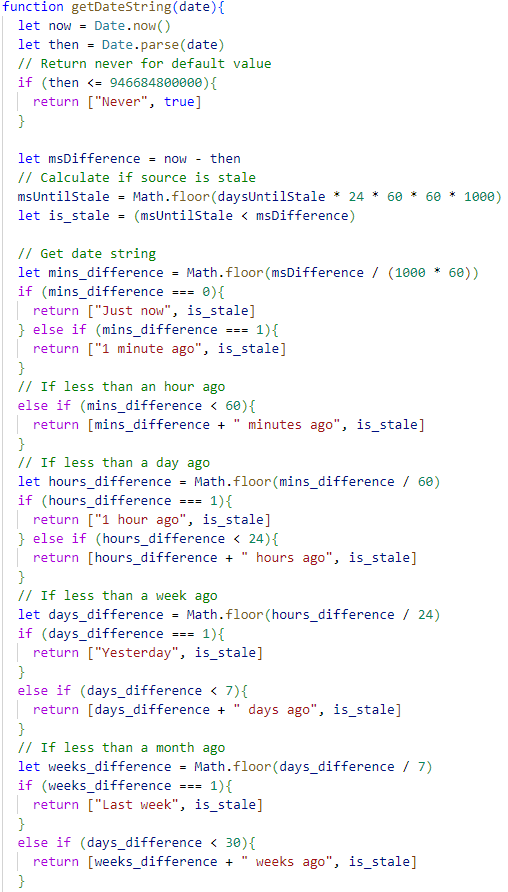
\includegraphics[width=0.7\textwidth]{images/JS_code1.png}
\end{figure}

 \begin{figure}[h]
\centering
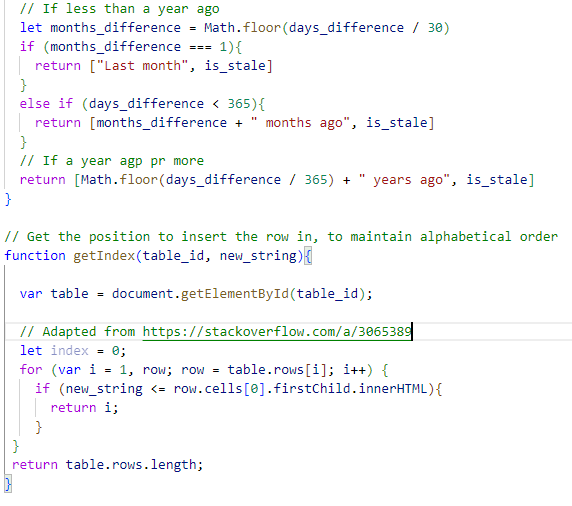
\includegraphics[width=0.7\textwidth]{images/JS_code2.png}
\end{figure}

 \begin{figure}[h]
\centering
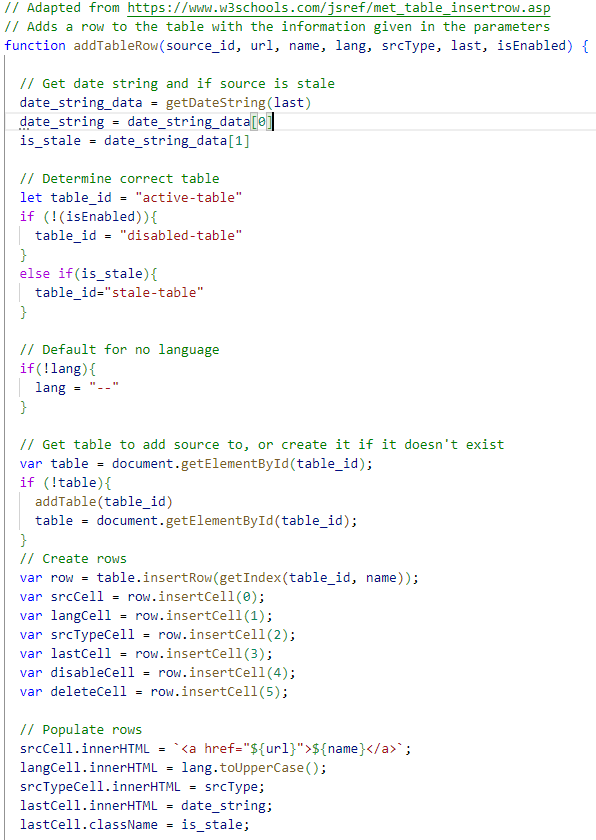
\includegraphics[width=0.7\textwidth]{images/JS_code3.png}
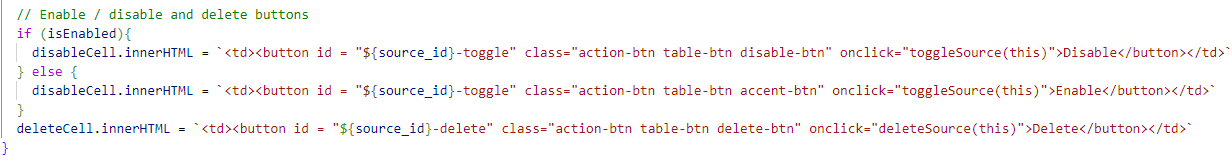
\includegraphics[width=\textwidth]{images/JS_code4.png}
\end{figure}


\chapter{Signed ethics checklist}
\label{appendix:ethics-checklist}
\begin{obeylines}
School of Computing Science
University of Glasgow

Ethics checklist form for assessed exercises (at all levels)

This form is only applicable for assessed exercises that use other people (‘participants’) for the collection of information, typically in getting comments about a system or a system design, or getting information about how a system could be used, or evaluating a working system.

If no other people have been involved in the collection of information, then you do not need to complete this form.

If your evaluation does not comply with any one or more of the points below, please contact the Chair of the School of Computing Science  Ethics Committee (matthew.chalmers@glasgow.ac.uk) for advice.

If your evaluation does comply with all the points below, please sign this form and submit it with your assessed work.

---------------------------------------------------------------------------------------------

1.	Participants were not exposed to any risks greater than those encountered in their normal working life.
Investigators have a responsibility to protect participants from physical and mental harm during the investigation. The risk of harm must be no greater than in ordinary life. Areas of potential risk that require ethical approval include, but are not limited to, investigations that occur outside usual laboratory areas, or that require participant mobility (e.g. walking, running, use of public transport), unusual or repetitive activity or movement, that use sensory deprivation (e.g. ear plugs or blindfolds), bright or flashing lights, loud or disorienting noises, smell, taste, vibration, or force feedback

2.	The experimental materials were paper-based, or comprised software running on standard hardware.
Participants should not be exposed to any risks associated with the use of non-standard equipment: anything other than pen-and-paper, standard PCs, laptops, iPads, mobile phones and common hand-held devices is considered non-standard.

3.	All participants explicitly stated that they agreed to take part, and that their data could be used in the project.
If the results of the evaluation are likely to be used beyond the term of the project (for example, the software is to be deployed, or the data is to be published), then signed consent is necessary. A separate consent form should be signed by each participant.

Otherwise, verbal consent is sufficient, and should be explicitly requested in the introductory script.

4.	No incentives were offered to the participants.
The payment of participants must not be used to induce them to risk harm beyond that which they risk without payment in their normal lifestyle. 
 
5.	No information about the evaluation or materials was intentionally withheld from the participants.
Withholding information or misleading participants is unacceptable if participants are likely to object or show unease when debriefed. 

6.	No participant was under the age of 16.
Parental consent is required for participants under the age of 16. 

7.	No participant has an impairment that may limit their understanding or communication.
Additional consent is required for participants with impairments. 

8.	Neither I nor my supervisor is in a position of authority or influence over any of the participants.
A position of authority or influence over any participant must not be allowed to pressurise participants to take part in, or remain in, any experiment. 

9.	All participants were informed that they could withdraw at any time.
All participants have the right to withdraw at any time during the investigation. They should be told this in the introductory script.

10.	All participants have been informed of my contact details.
All participants must be able to contact the investigator after the investigation. They should be given the details of both student and module co-ordinator or supervisor as part of the debriefing.

11.	The evaluation was discussed with all the participants at the end of the session, and all participants had the opportunity to ask questions.
The student must provide the participants with sufficient information in the debriefing to enable them to understand the nature of the investigation. In cases where remote participants may withdraw from the experiment early and it is not possible to debrief them, the fact that doing so will result in their not being debriefed should be mentioned in the introductory text.

12.	All the data collected from the participants is stored in an anonymous form.
All participant data (hard-copy and soft-copy) should be stored securely, and in anonymous form. 
---------------------------------------------------------------------------------------------

Course and Assessment Name: \underline{COMPSCI402SP: Level 4 Individual Project}
Student’s Name: \underline{Adam Fairlie}
Student Number: \underline{2461352}
Student’s Signature: \underline{Adam Fairlie}
Date \underline{19/03/2023}
\end{obeylines}


\chapter{Questionnaire}
\label{appendix:questionnaire}

 \begin{figure}[h]
\centering
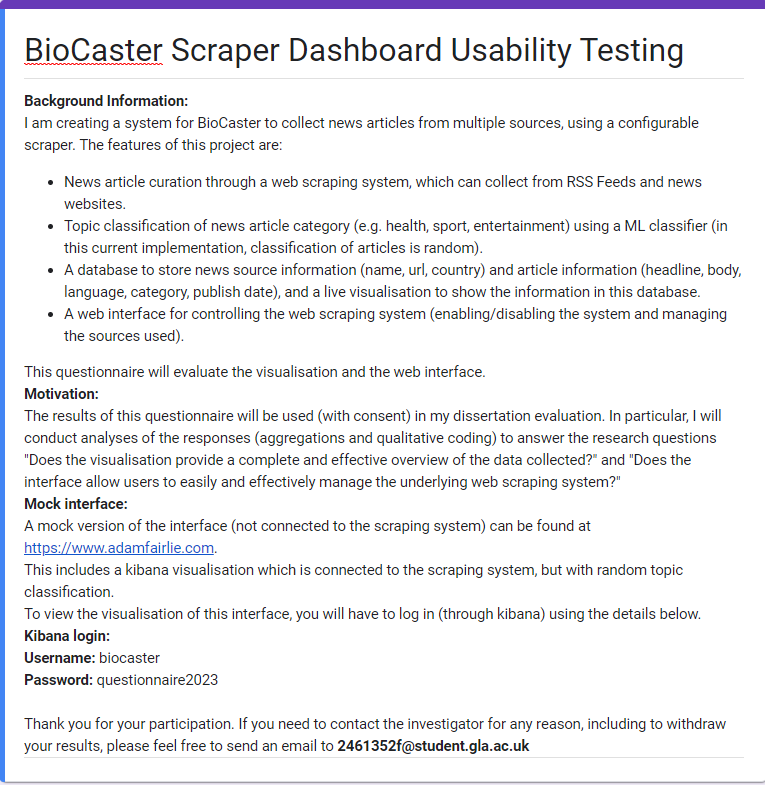
\includegraphics[width=\textwidth]{images/Form1.png}
\end{figure}

 \begin{figure}[h]
\centering
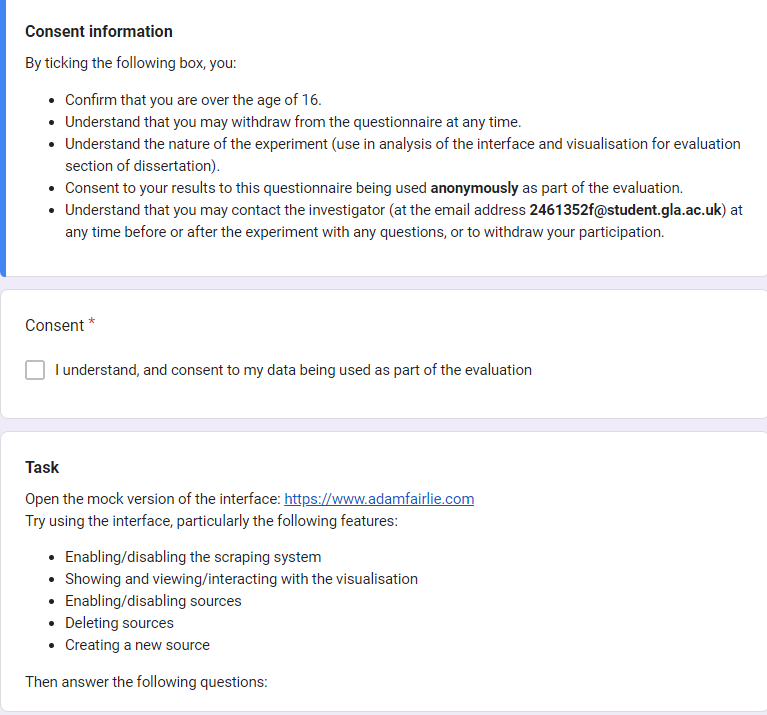
\includegraphics[width=\textwidth]{images/Form2.png}
\end{figure}

 \begin{figure}[h]
\centering
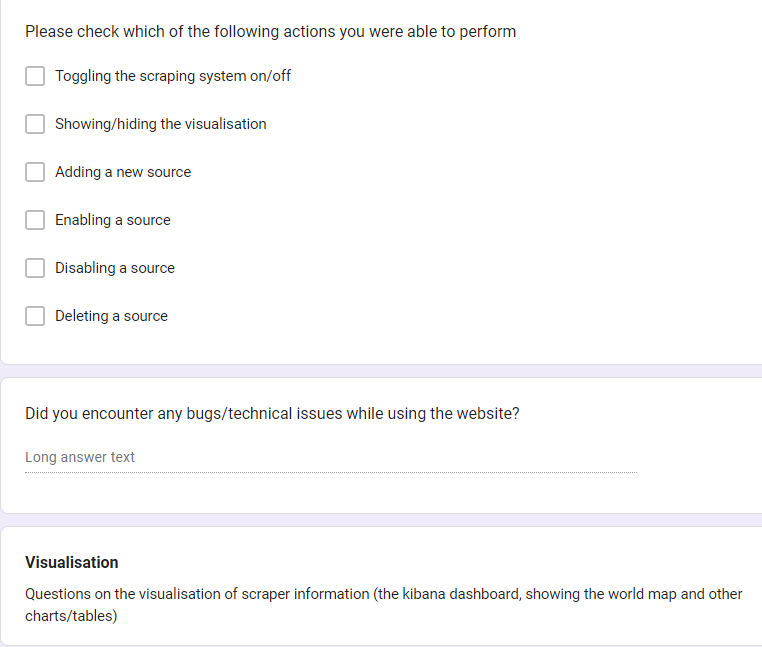
\includegraphics[width=\textwidth]{images/Form3.png}
\end{figure}

 \begin{figure}[h]
\centering
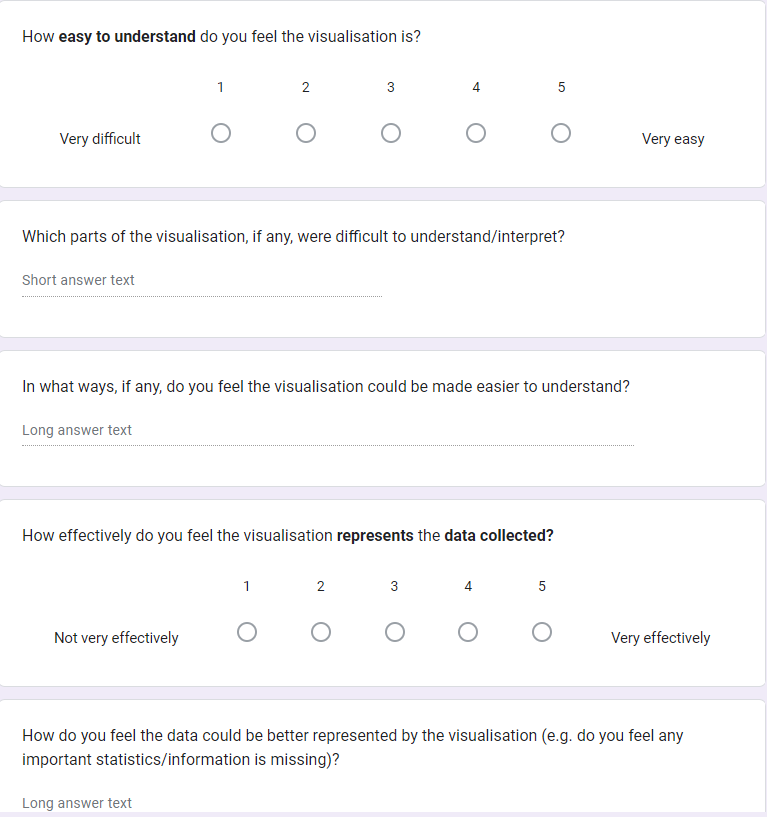
\includegraphics[width=\textwidth]{images/Form4.png}
\end{figure}

 \begin{figure}[h]
\centering
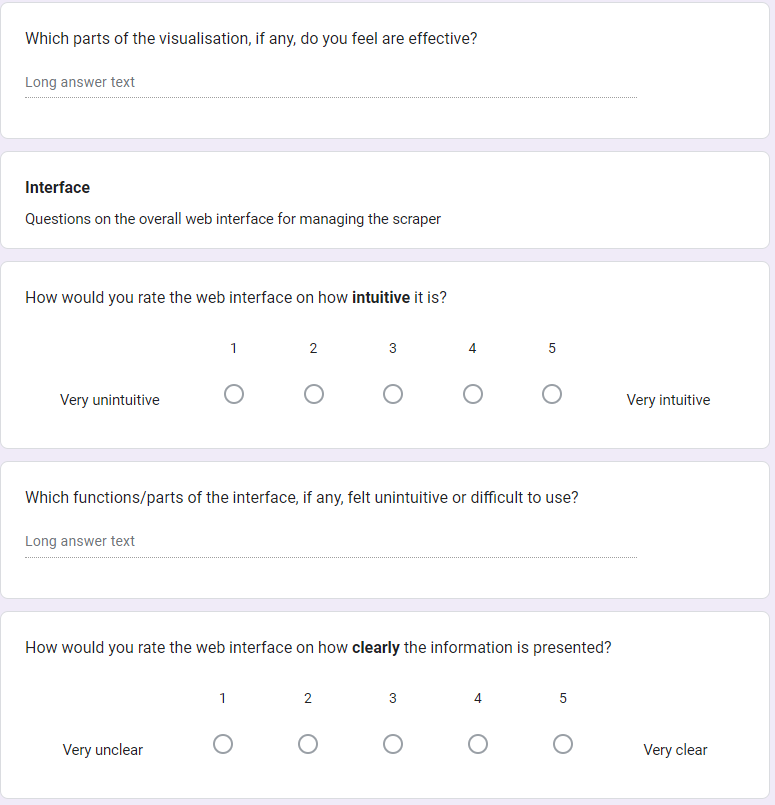
\includegraphics[width=\textwidth]{images/Form5.png}
\end{figure}

 \begin{figure}[h]
\centering
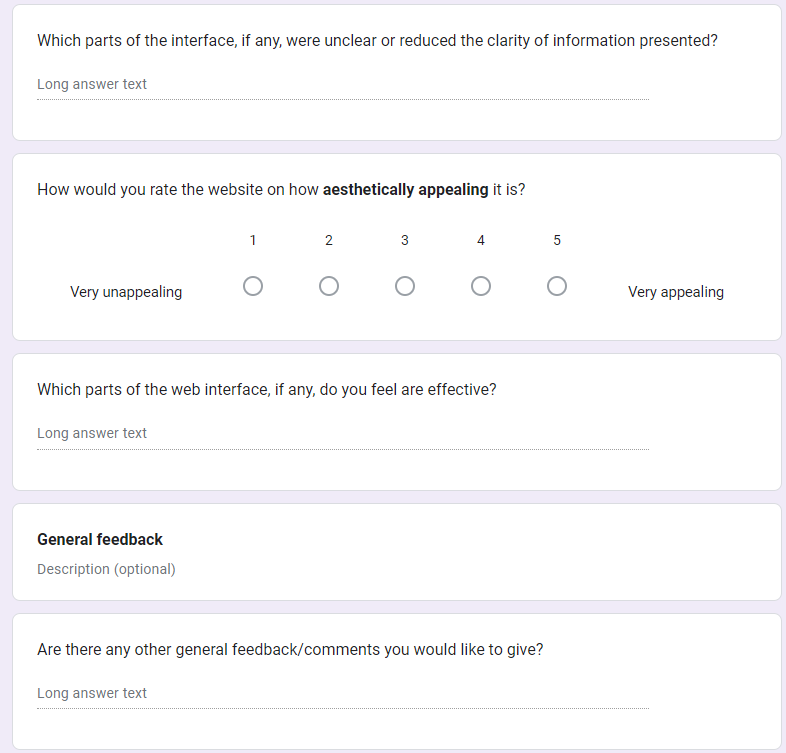
\includegraphics[width=\textwidth]{images/Form6.png}
\end{figure}

\end{appendices}

%==================================================================================================================================
%   BIBLIOGRAPHY   
\bibliographystyle{abbrvnat}
\bibliography{l4proj}

\end{document}
